\documentclass{beamer}
\usetheme[faculty=med]{fibeamer}
\usepackage[utf8]{inputenc}
\usepackage[
  main=english
]{babel}        %% typeset as follows:
%% These macros specify information about the presentation
\title{Sistemas Operacionais} %% that will be typeset on the
\subtitle{Comunicação interprocessos} %% title page.
\author{Guilherme Meira}
%% These additional packages are used within the document:
\usepackage{ragged2e}  % `\justifying` text
\usepackage{booktabs}  % Tables
\usepackage{tabularx}
\usepackage{tikz}      % Diagrams
\usetikzlibrary{calc, shapes, backgrounds, positioning}
\usepackage{minted}
\usepackage{amsmath, amssymb}
\usepackage{url}       % `\url`s
\usepackage{listings}  % Code listings
\usepackage{xcolor}
\definecolor{highlightcolor}{RGB}{255, 140, 119}
\setminted{highlightcolor=highlightcolor}
\frenchspacing
\begin{document}
  \frame{\maketitle}
  \AtBeginSection[]{% Print an outline at the beginning of sections
  	\begin{frame}<beamer>
  		\frametitle{Agenda}
  		\tableofcontents[currentsection]
  	\end{frame}}
  	
\section{Introdução}
\begin{frame}{Introdução}
   	\begin{itemize}
   		\item Frequentemente, processos precisam se comunicar para realizar suas tarefas
   		\begin{itemize}
   			\item Um processo precisa compartilhar informações com outro
   			\item Um processo precisa garantir que não vai atrapalhar o outro
   			\begin{itemize}
   				\item Exemplo: reserva do último assento em um avião
   			\end{itemize}
   			\item A sequência de execução dos processos deve respeitar a dependência entre eles
   			\begin{itemize}
   				\item Se o processo A produz dados e o processo B imprime os dados, o processo B precisa esperar até que A tenha produzido algum dado
   			\end{itemize}
   		\end{itemize}
   		\item O segundo e o terceiro problema também se aplicam a threads (o problema da comunicação é resolvido utilizando o espaço de endereçamento compartilhado)
   	\end{itemize}
\end{frame}
\section{Condições de corrida}
\begin{frame}{Condições de corrida}
	\begin{itemize}
		\item \textbf{Exemplo:} spooler de impressão
	\end{itemize}
	\begin{figure}
		\only<1>{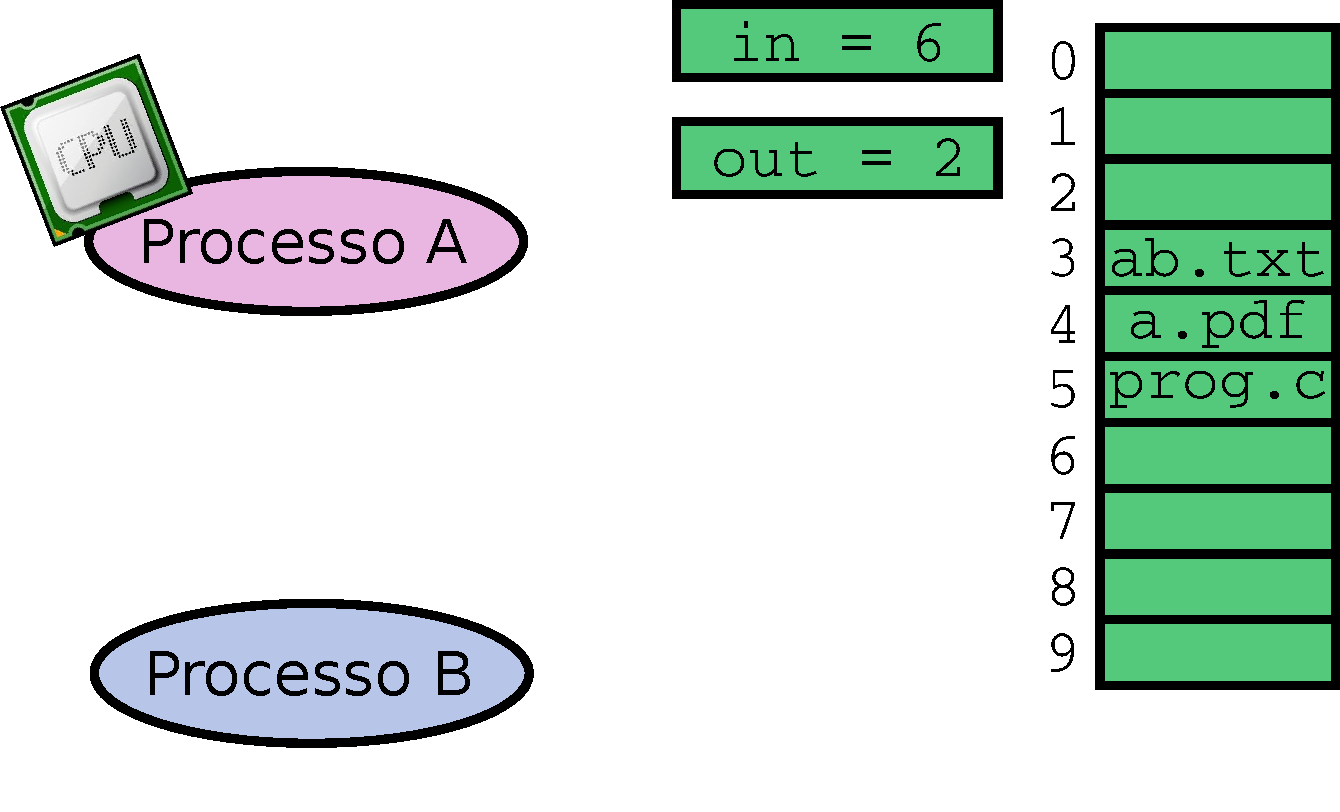
\includegraphics[width=0.6\paperwidth]{resources/race1}}
		\only<2>{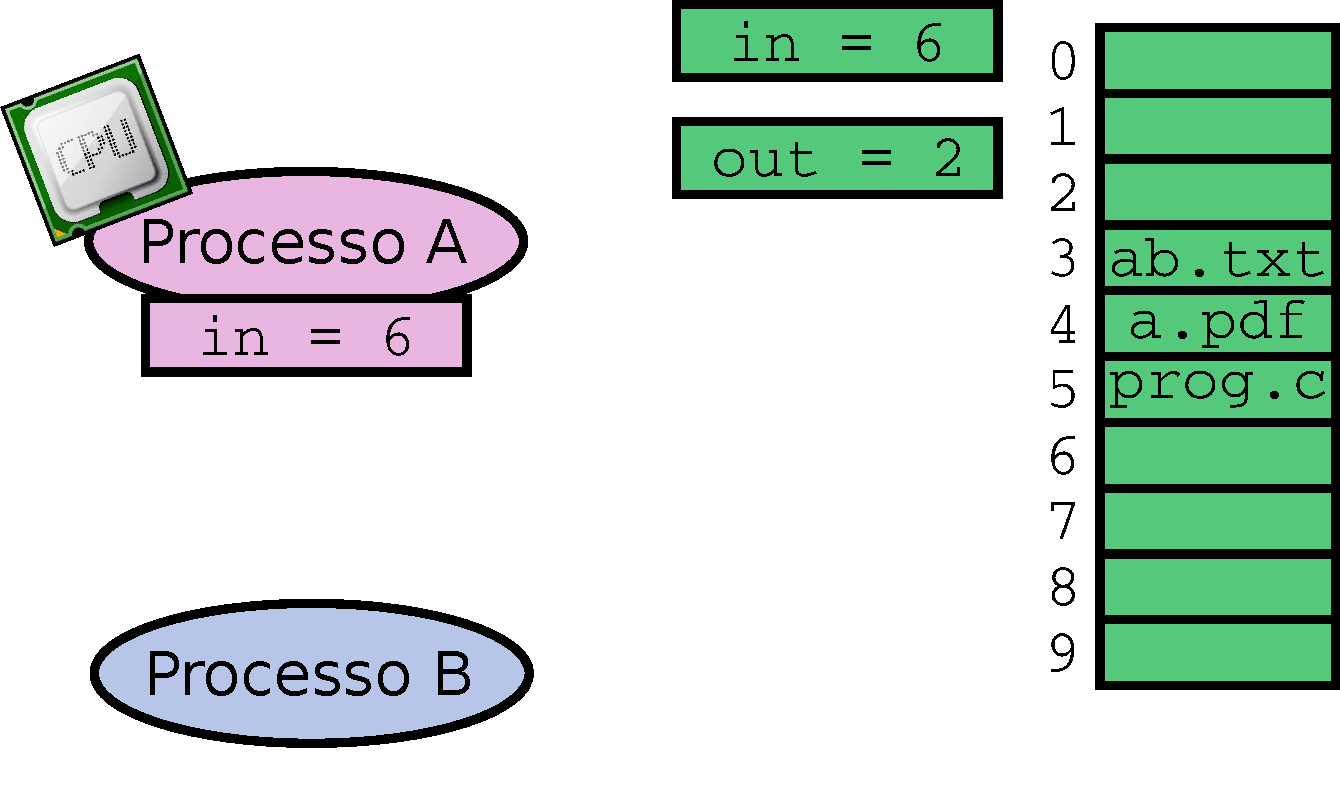
\includegraphics[width=0.6\paperwidth]{resources/race2}}
		\only<3>{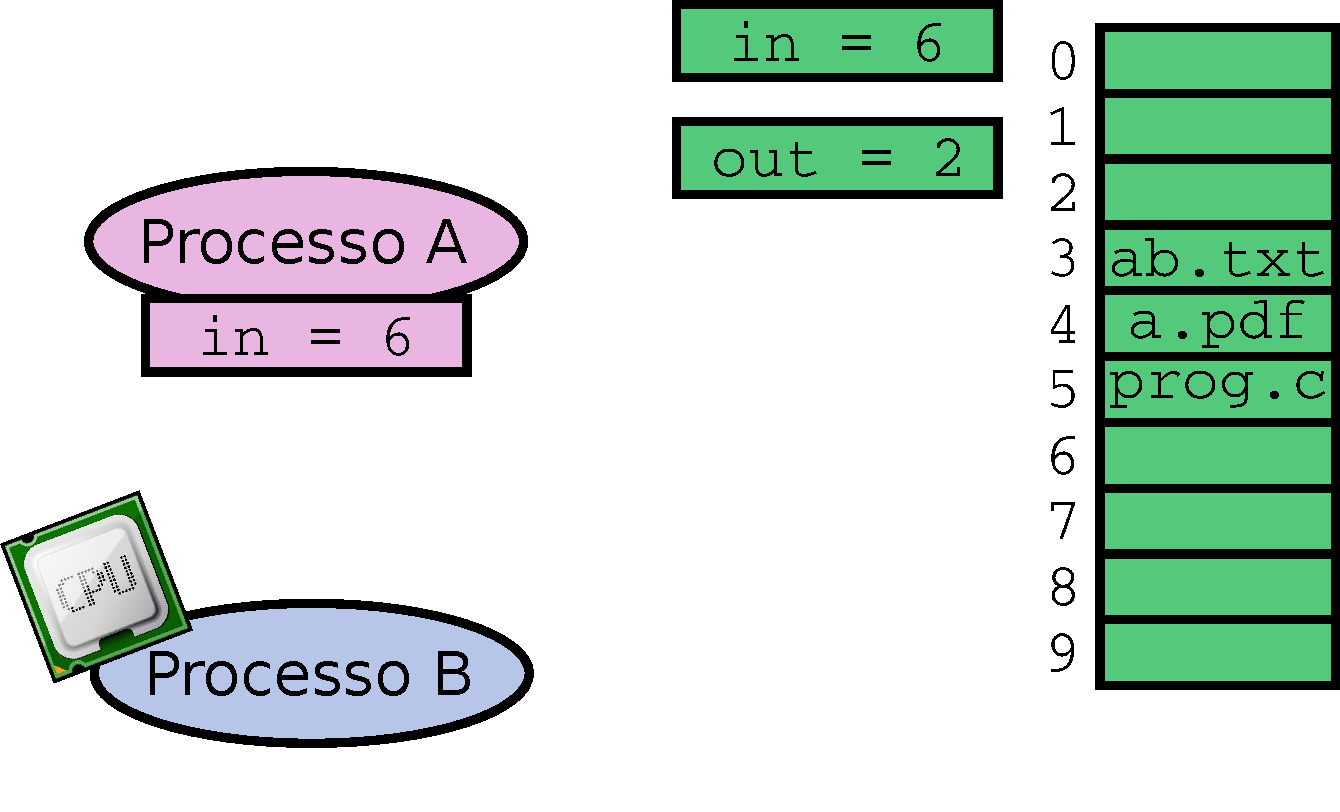
\includegraphics[width=0.6\paperwidth]{resources/race3}}
		\only<4>{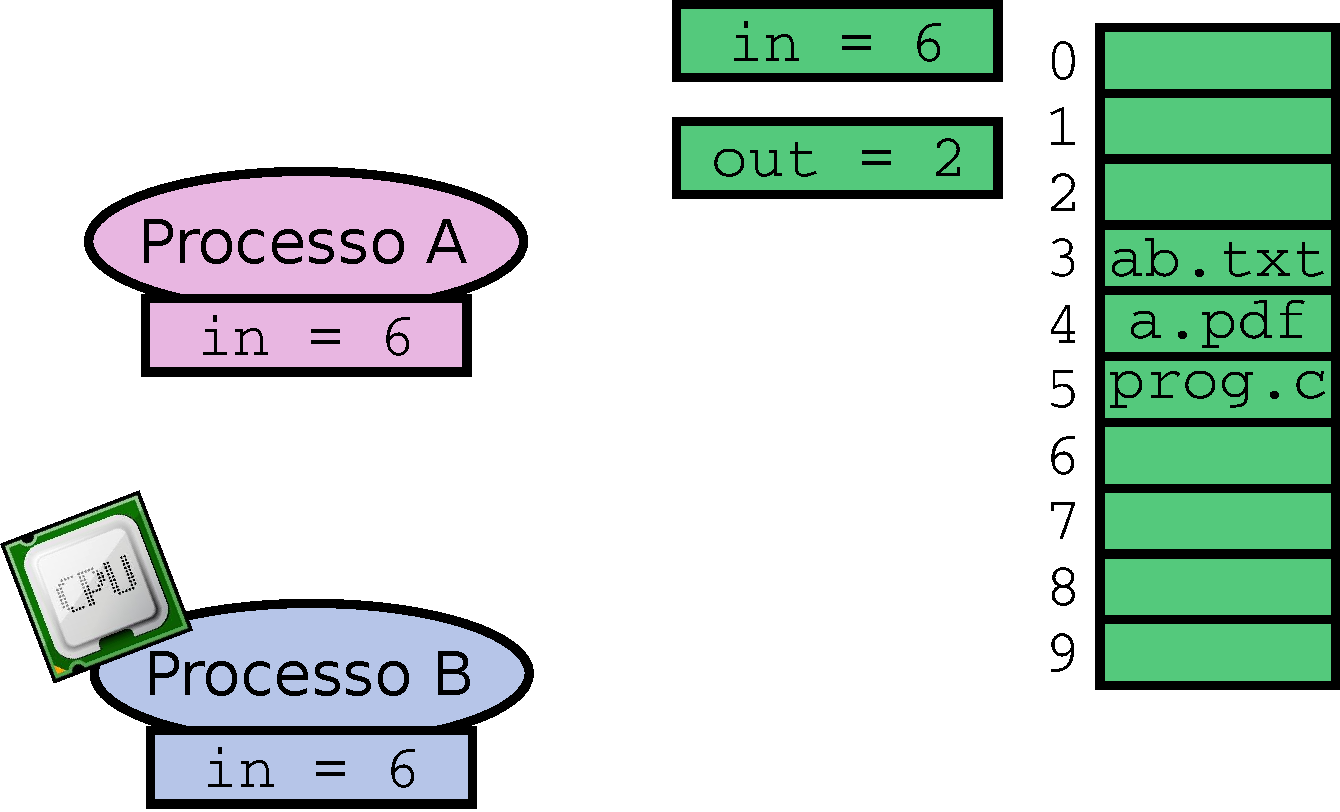
\includegraphics[width=0.6\paperwidth]{resources/race4}}
		\only<5>{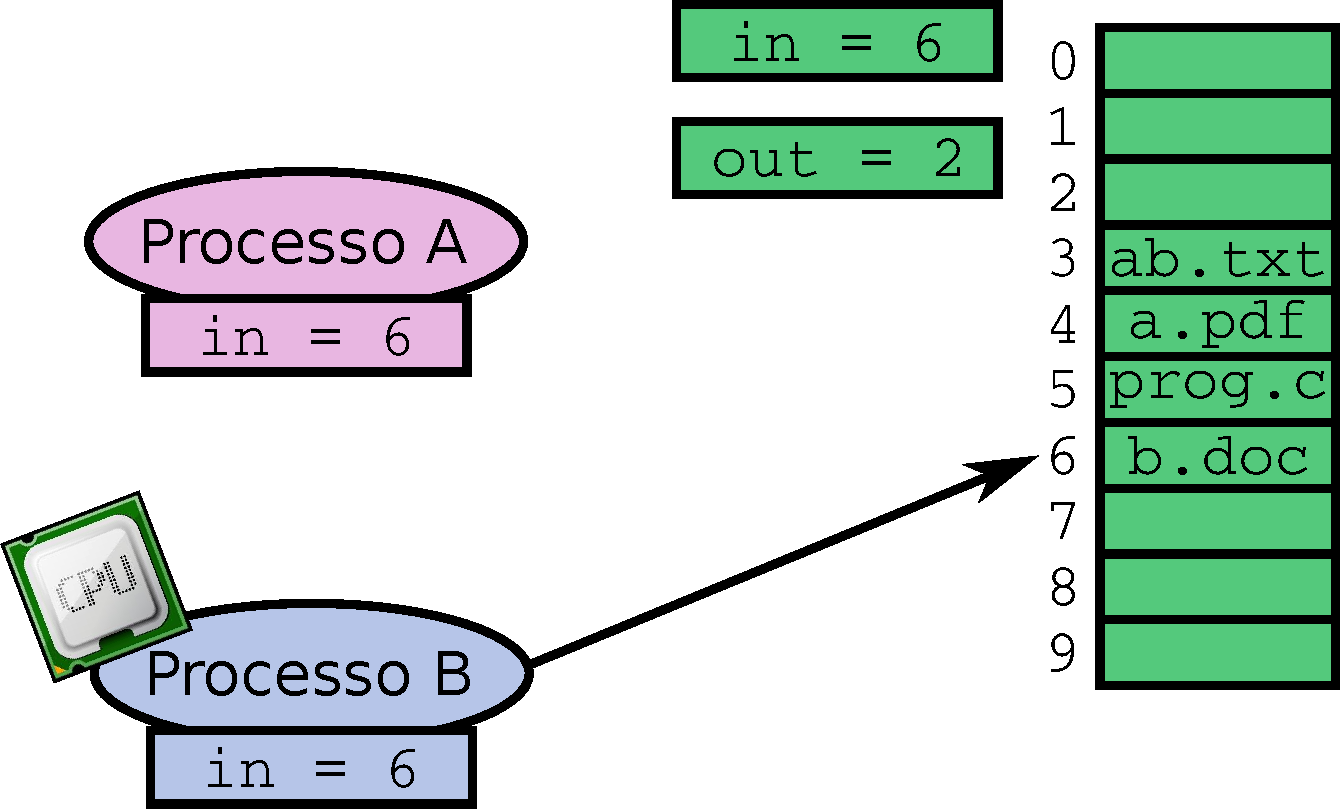
\includegraphics[width=0.6\paperwidth]{resources/race5}}
		\only<6>{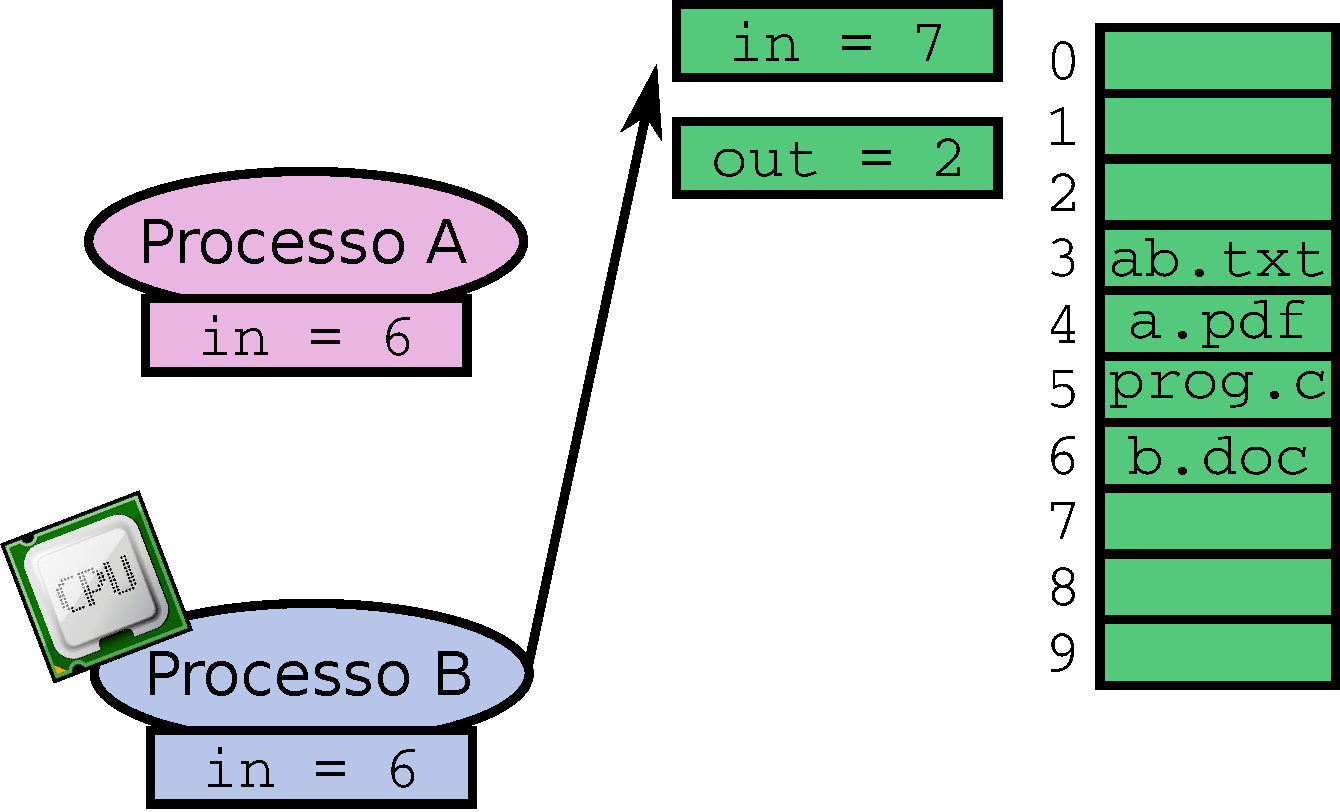
\includegraphics[width=0.6\paperwidth]{resources/race6}}
		\only<7>{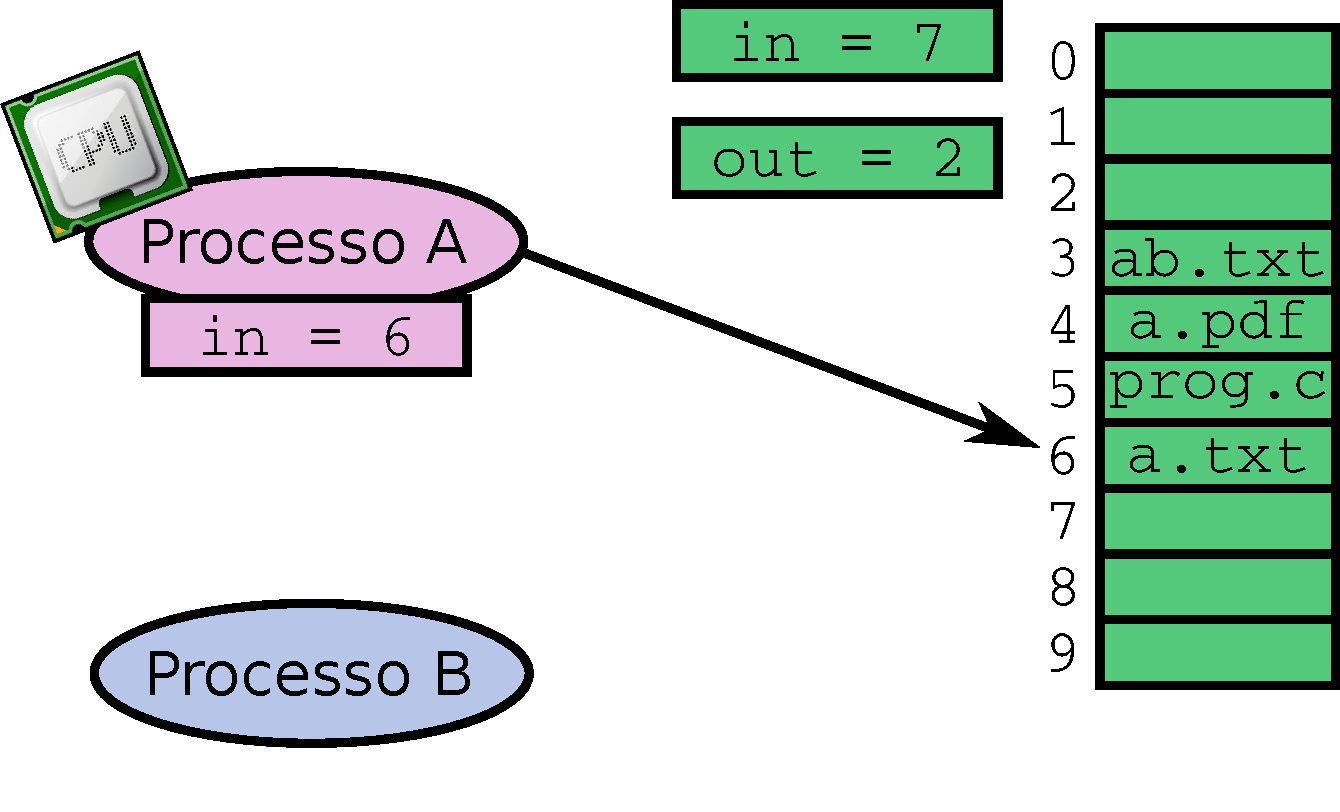
\includegraphics[width=0.6\paperwidth]{resources/race7}}
		\only<8>{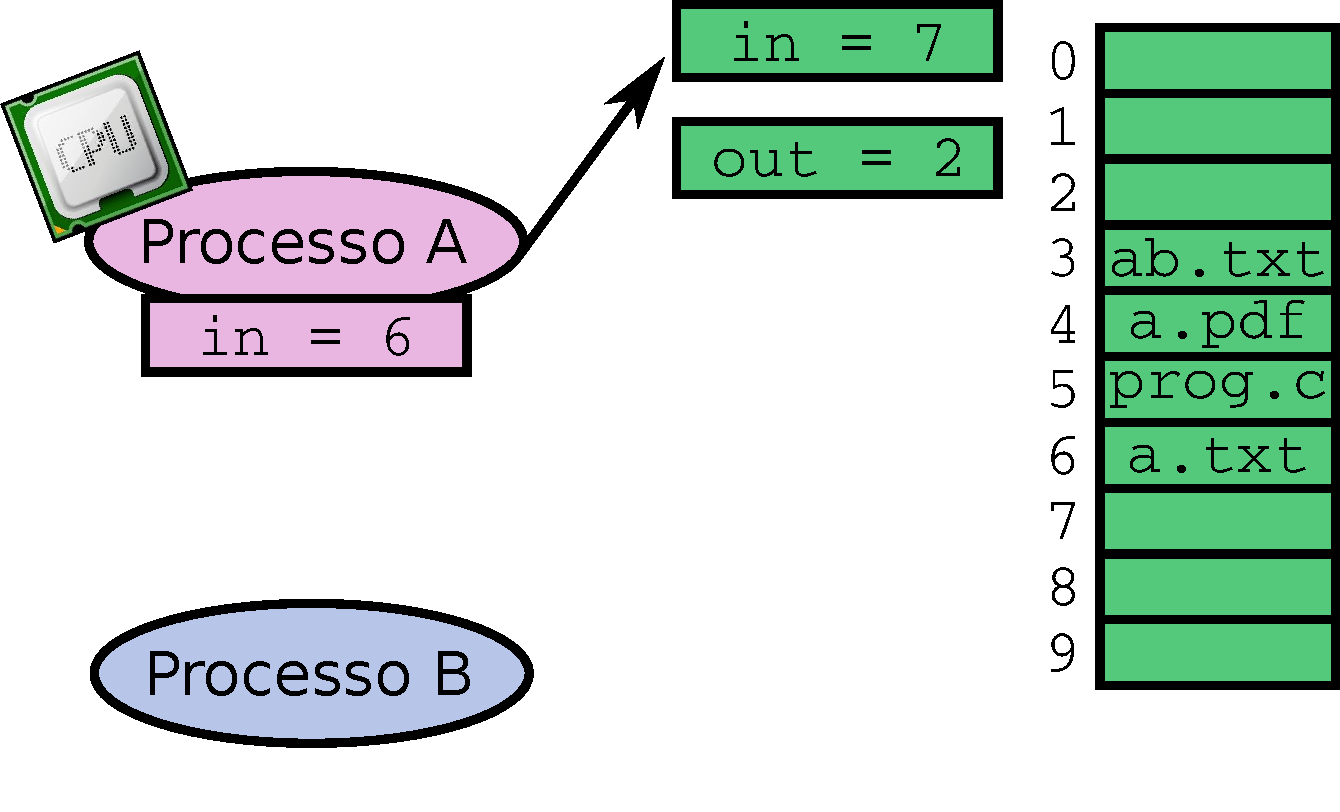
\includegraphics[width=0.6\paperwidth]{resources/race8}}
	\end{figure}
\end{frame}
\begin{frame}{Condições de corrida}
	\begin{itemize}
		\item Condições de corrida ocorrem quando processos acessam dados compartilhados e o resultado final depende da sequência exata em que os processos foram executados
		\item São extremamente difíceis de debugar, pois só ocorrem em situações muito específicas
	\end{itemize}
\end{frame}
\begin{frame}{Condições de corrida}
	\begin{itemize}
		\item Para evitar condições de corrida, devemos proibir o acesso simultâneo a dados que estejam acessíveis por vários processos. Precisamos de um mecanismo de \textbf{exclusão mútua}
		\item As regiões dos programas que acessam os dados compartilhados são chamadas de \textbf{regiões críticas}. Precisamos de mecanismos que impeçam dois processos de entrarem em suas regiões críticas ao mesmo tempo
	\end{itemize}
\end{frame}
\begin{frame}{Condições de corrida}
	\begin{itemize}
		\item Uma boa solução deve atender aos requisitos:
		\begin{itemize}
			\item Dois processos nunca podem acessar suas regiões críticas simultaneamente
			\item Não podemos assumir nada a respeito da velocidade ou do número de CPUs
			\item Nenhum processo fora de sua região crítica deve bloquear outros processos
			\item Nenhum processo deve ter que esperar para sempre para entrar em sua região crítica
		\end{itemize}
	\end{itemize}
\end{frame}
\begin{frame}{Condições de corrida}
	\begin{figure}
		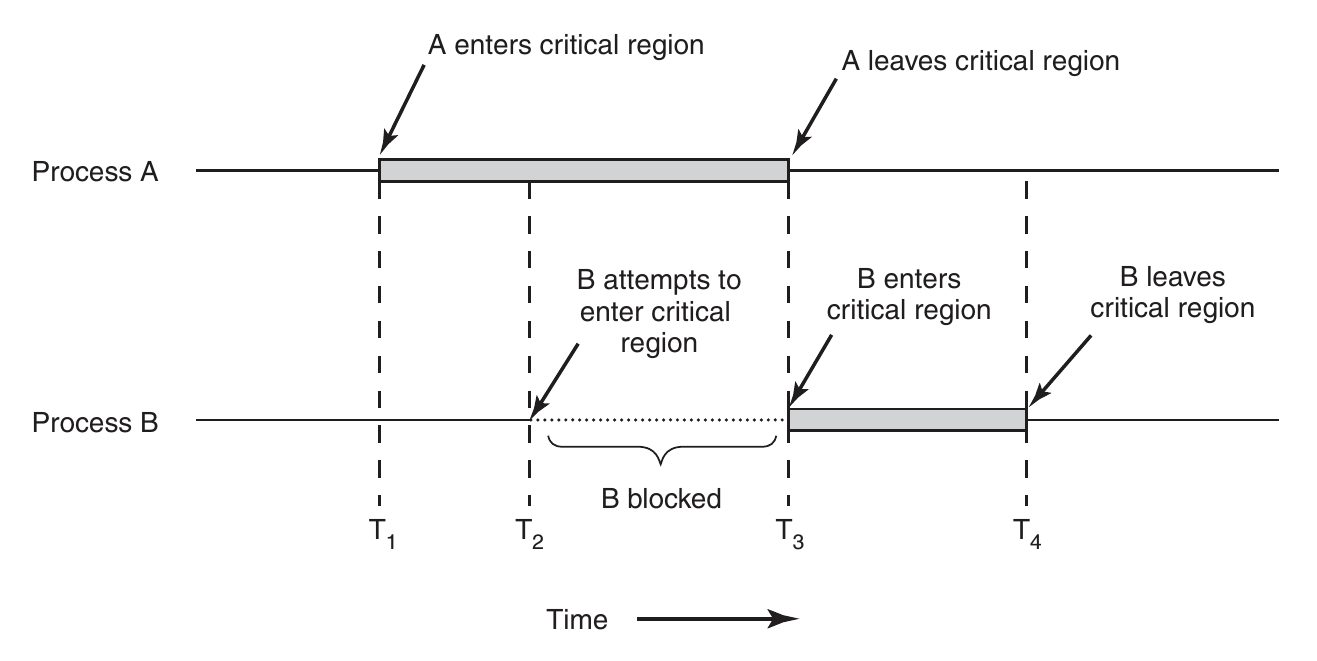
\includegraphics[width=0.9\paperwidth]{resources/critical}
	\end{figure}
\end{frame}
\begin{frame}{Condições de corrida}
	\framesubtitle{Exclusão mútua com espera ocupada}
	\begin{itemize}
		\item Uma primeira ideia: \textbf{desabilitar interrupções}
		\begin{itemize}
			\item A troca de processos na CPU realizada pelo sistema operacional depende diretamente de uma interrupção
			\item Com interrupções desabilitadas, o processo nunca será interrompido\pause
			\item \textbf{Problemas:}
			\begin{itemize}
				\item Se o processo não reabilitar as interrupções, ele assume controle total da CPU para sempre
				\item Pode ser conveniente para o kernel em situações específicas
				\item Não funciona para máquinas com múltiplas CPUs
			\end{itemize}
		\end{itemize}
	\end{itemize}
\end{frame}
\begin{frame}{Condições de corrida}
	\framesubtitle{Exclusão mútua com espera ocupada}
	\begin{itemize}
		\item \textbf{Variáveis de trava (lock)}
		\begin{itemize}
			\item Utilizar uma variável compartilhada indicando se algum processo está em sua região crítica
			\item Quando a variável é zero, nenhum processo está na região crítica
			\item Antes de entrar na região crítica, o processo verifica essa variável. Se for zero, ela é setada para 1 e o processo entra na região crítica\pause
			\item \textbf{Problemas:}
			\begin{itemize}
				\item Os mesmos de antes
			\end{itemize}
		\end{itemize}
	\end{itemize}
\end{frame}
\begin{frame}{Condições de corrida}
	\framesubtitle{Exclusão mútua com espera ocupada}
	\begin{itemize}
		\item \textbf{Chaveamento obrigatório}
		\begin{columns}
			\begin{column}{0.5\textwidth}
				\inputminted{c}{resources/strictalternation1.c}
			\end{column}
			\begin{column}{0.5\textwidth}
				\inputminted{c}{resources/strictalternation2.c}
			\end{column}
		\end{columns}
	\end{itemize}
\end{frame}
\begin{frame}{Condições de corrida}
	\framesubtitle{Exclusão mútua com espera ocupada}
	\begin{itemize}
		\item \textbf{Chaveamento obrigatório}
		\begin{itemize}
			\item Consegue evitar condições de corrida\pause
			\item \textbf{Problemas:}
			\begin{itemize}
				\item Os processos obrigatoriamente precisam alternar entre si. Um processo não pode entrar duas vezes seguidas na região crítica
				\item Viola a condição 3 (um processo fora da região crítica pode bloquear outros processos)
				\item Espera ocupada gasta ciclos da CPU desnecessariamente
			\end{itemize}
		\end{itemize}
	\end{itemize}
\end{frame}
\begin{frame}{Condições de corrida}
	\framesubtitle{Exclusão mútua com espera ocupada}
	\begin{itemize}
		\item \textbf{Solução de Peterson}
		\inputminted[fontsize=\footnotesize]{c}{resources/peterson.c}
	\end{itemize}
\end{frame}
\begin{frame}{Condições de corrida}
	\framesubtitle{Exclusão mútua com espera ocupada}
	\begin{itemize}
		\item \textbf{A instrução TSL}
		\begin{itemize}
			\item Esta solução requer ajuda do hardware
			\item \textbf{TSL:} test and set lock
			\item A instrução tem o formato:
			
			\texttt{TSL RX, LOCK}
			\item A instrução lê o conteúdo da posição de memória \texttt{LOCK} para o registrador \texttt{RX} e armazena um valor diferente de zero na posição \texttt{LOCK}
			\item Durante a execução dessa instrução, o barramento de memória é bloqueado, garantindo que nenhuma outra CPU acesse a memória
		\end{itemize}
	\end{itemize}
\end{frame}
\begin{frame}{Condições de corrida}
	\framesubtitle{Exclusão mútua com espera ocupada}
	\begin{itemize}
		\item \textbf{A instrução TSL}
		\inputminted{c}{resources/tsl.asm}
	\end{itemize}
\end{frame}
\begin{frame}{Condições de corrida}
	\framesubtitle{Exclusão mútua com espera ocupada}
	\begin{itemize}
		\item \textbf{A instrução XCHG}
		\begin{itemize}
			\item A instrução \texttt{XCHG} está presente em CPUs x86 da Intel
			\item Ela troca os valores de uma posição de memória e um registrador e pode ser usada de maneira semelhante à \texttt{TSL}
		\end{itemize}
	\end{itemize}
\end{frame}
\begin{frame}{Condições de corrida}
	\framesubtitle{Exclusão mútua com espera ocupada}
	\begin{itemize}
		\item \textbf{A instrução XCHG}
		\inputminted{c}{resources/xchg.asm}
	\end{itemize}
\end{frame}
\begin{frame}{Condições de corrida}
	\framesubtitle{Sleep e wakeup}
	\begin{itemize}
		\item Até então, todas as soluções envolveram espera ocupada, isto é, o processo sempre fica em um loop checando o valor de uma variável, desperdiçando ciclos de CPU
		\item Vamos investigar soluções que bloqueiam o processo quando ele tenta entrar na região crítica e outro processo já está lá
		\item Imagine duas chamadas de sistema:
		\begin{itemize}
			\item \textbf{\texttt{sleep}:} faz com que o processo que a chamou bloqueie
			\item \textbf{\texttt{wakeup}:} recebe um parâmetro, o número do processo a ser acordado
		\end{itemize}
	\end{itemize}
\end{frame}
\begin{frame}{Condições de corrida}
	\framesubtitle{Sleep e wakeup}
	\begin{itemize}
		\item \textbf{O problema do produtor-consumidor:}
	\end{itemize}
	\begin{figure}
		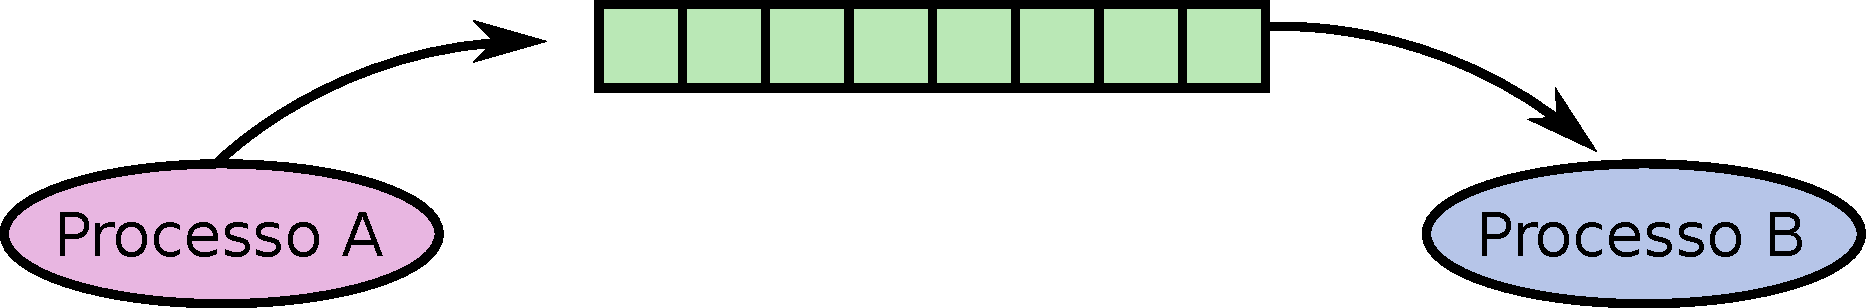
\includegraphics[width=0.8\paperwidth]{resources/producerconsumer}
	\end{figure}
\end{frame}
\begin{frame}{Condições de corrida}
	\framesubtitle{Sleep e wakeup}
	\begin{itemize}
		\item \textbf{O problema do produtor-consumidor:}
		\begin{itemize}
			\item O processo A coloca dados no buffer enquanto o processo B retira os dados
			\item O problema surge quando o buffer está cheio e A tenta inserir ou quando o buffer está vazio e B tenta ler
			\item Podemos utilizar uma variável para armazenar o número de elementos do buffer, mas isso leva às mesmas condições de corrida que já vimos anteriormente
		\end{itemize}
	\end{itemize}
\end{frame}
\begin{frame}{Condições de corrida}
	\framesubtitle{Sleep e wakeup}
	\begin{itemize}
		\item \textbf{O problema do produtor-consumidor:}
		\begin{columns}
			\begin{column}{0.5\textwidth}
				\inputminted[fontsize=\footnotesize]{c}{resources/producer.c}
			\end{column}
			\begin{column}{0.5\textwidth}
				\inputminted[fontsize=\footnotesize]{c}{resources/consumidor.c}
			\end{column}
		\end{columns}
	\end{itemize}
\end{frame}
\begin{frame}{Condições de corrida}
	\framesubtitle{Sleep e wakeup}
	\begin{itemize}
		\item \textbf{O problema do produtor-consumidor:}
		\begin{itemize}
			\item Podemos corrigir esse problema alterando o comportamento das funções \texttt{sleep} e \texttt{wakeup}
			\item Podemos utilizar um bit para dizer se um \texttt{wakeup} foi enviado, mas o processo ainda estava acordado
			\item Quando o processo chama \texttt{sleep}, se esse bit é 1, ele é setado para zero e o processo não dorme
			\item Resolve o problema para dois processos, mas não para vários
		\end{itemize}
	\end{itemize}
\end{frame}
\begin{frame}{Condições de corrida}
	\framesubtitle{Semáforos}
	\begin{itemize}
		\item Propostos por Dijkstra em 1965
		\item Semáforos são variáveis que armazenam quantos \texttt{wakeup}s estamos ``guardando''
		\item Só podem ser manipulados por duas operações:
		\begin{itemize}
			\item \textbf{down:} decrementa o semáforo, \textbf{bloqueia} o processo se o semáforo for zero
			\item \textbf{up:} incrementa o semáforo, \textbf{acorda} um dos processos que estejam bloqueados neste semáforo
		\end{itemize}
		\item Ambas as operações devem ser \textbf{atômicas}, isto é, um processo não pode ser interrompido enquanto as executa
	\end{itemize}
\end{frame}
\begin{frame}{Condições de corrida}
	\framesubtitle{Sleep e wakeup}
	\begin{itemize}
		\item \textbf{O problema do produtor-consumidor:}
		\begin{columns}
			\begin{column}{0.5\textwidth}
				\inputminted[fontsize=\footnotesize,lastline=14]{c}{resources/semaforo.c}
			\end{column}
			\begin{column}{0.5\textwidth}
				\inputminted[fontsize=\footnotesize,firstline=16]{c}{resources/semaforo.c}
			\end{column}
		\end{columns}
	\end{itemize}
\end{frame}
\begin{frame}{Condições de corrida}
	\begin{figure}
		\only<1>{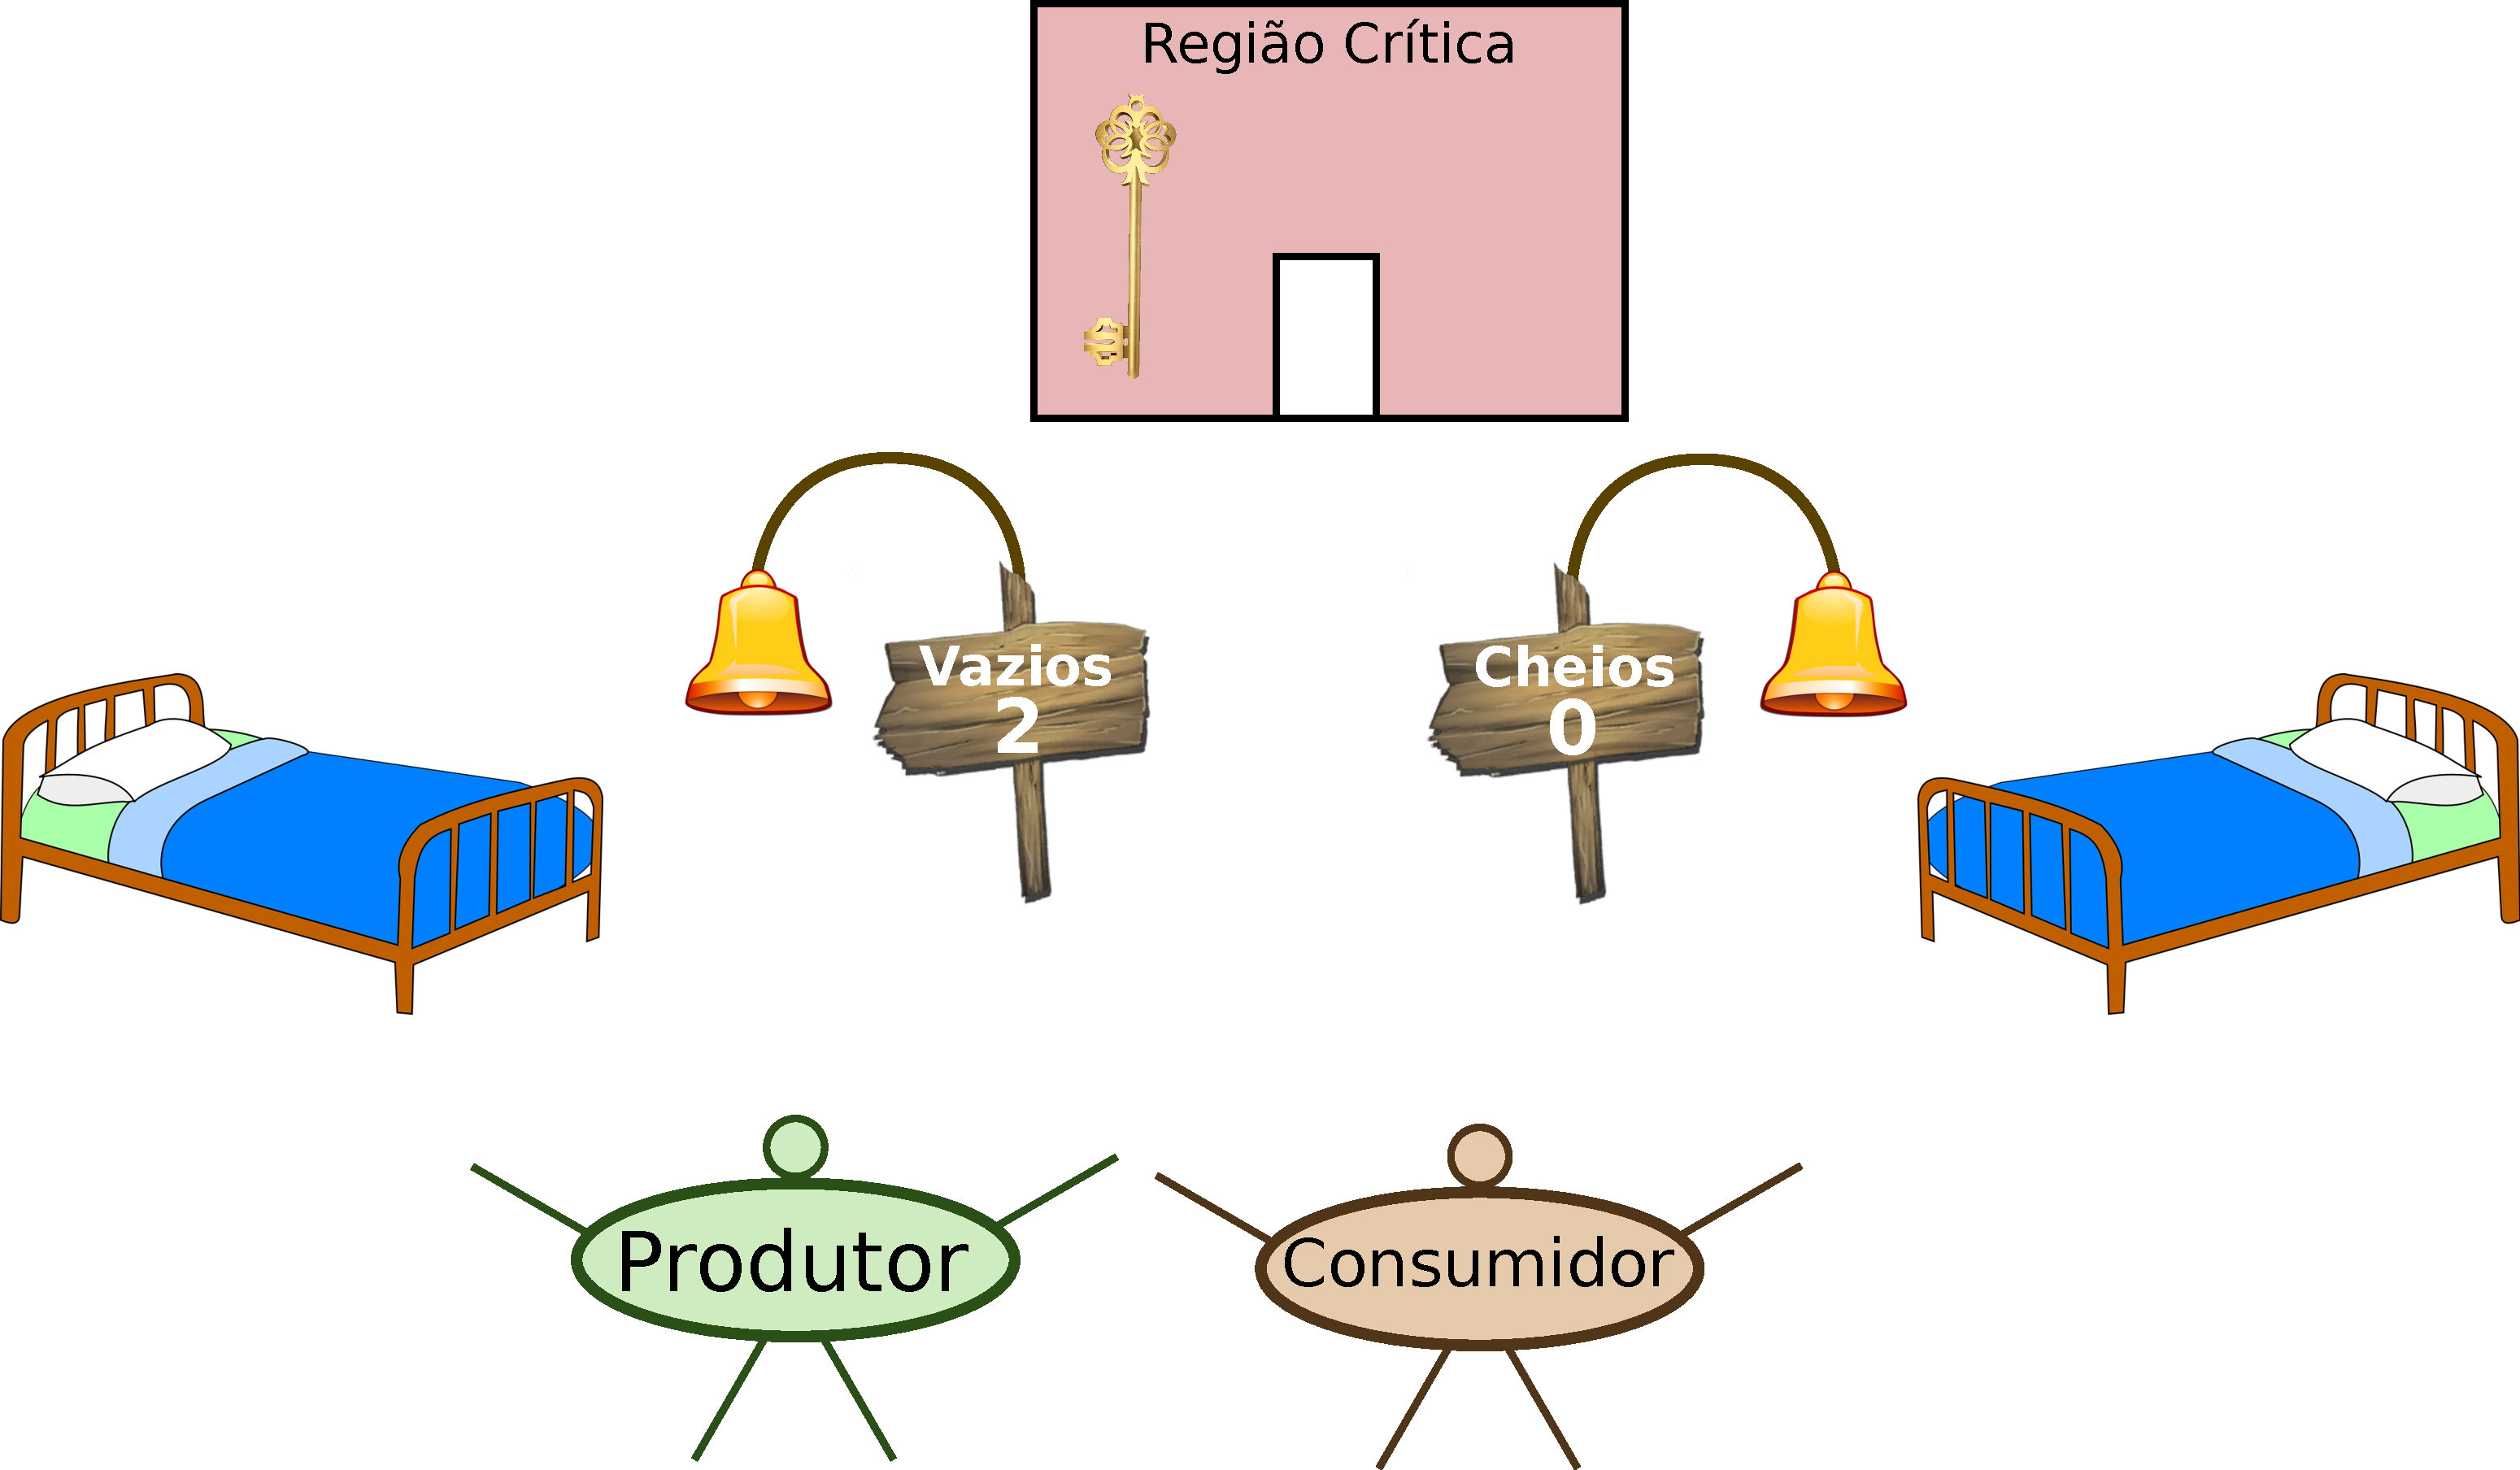
\includegraphics[width=0.9\paperwidth]{resources/semaphore1}}
		\only<2>{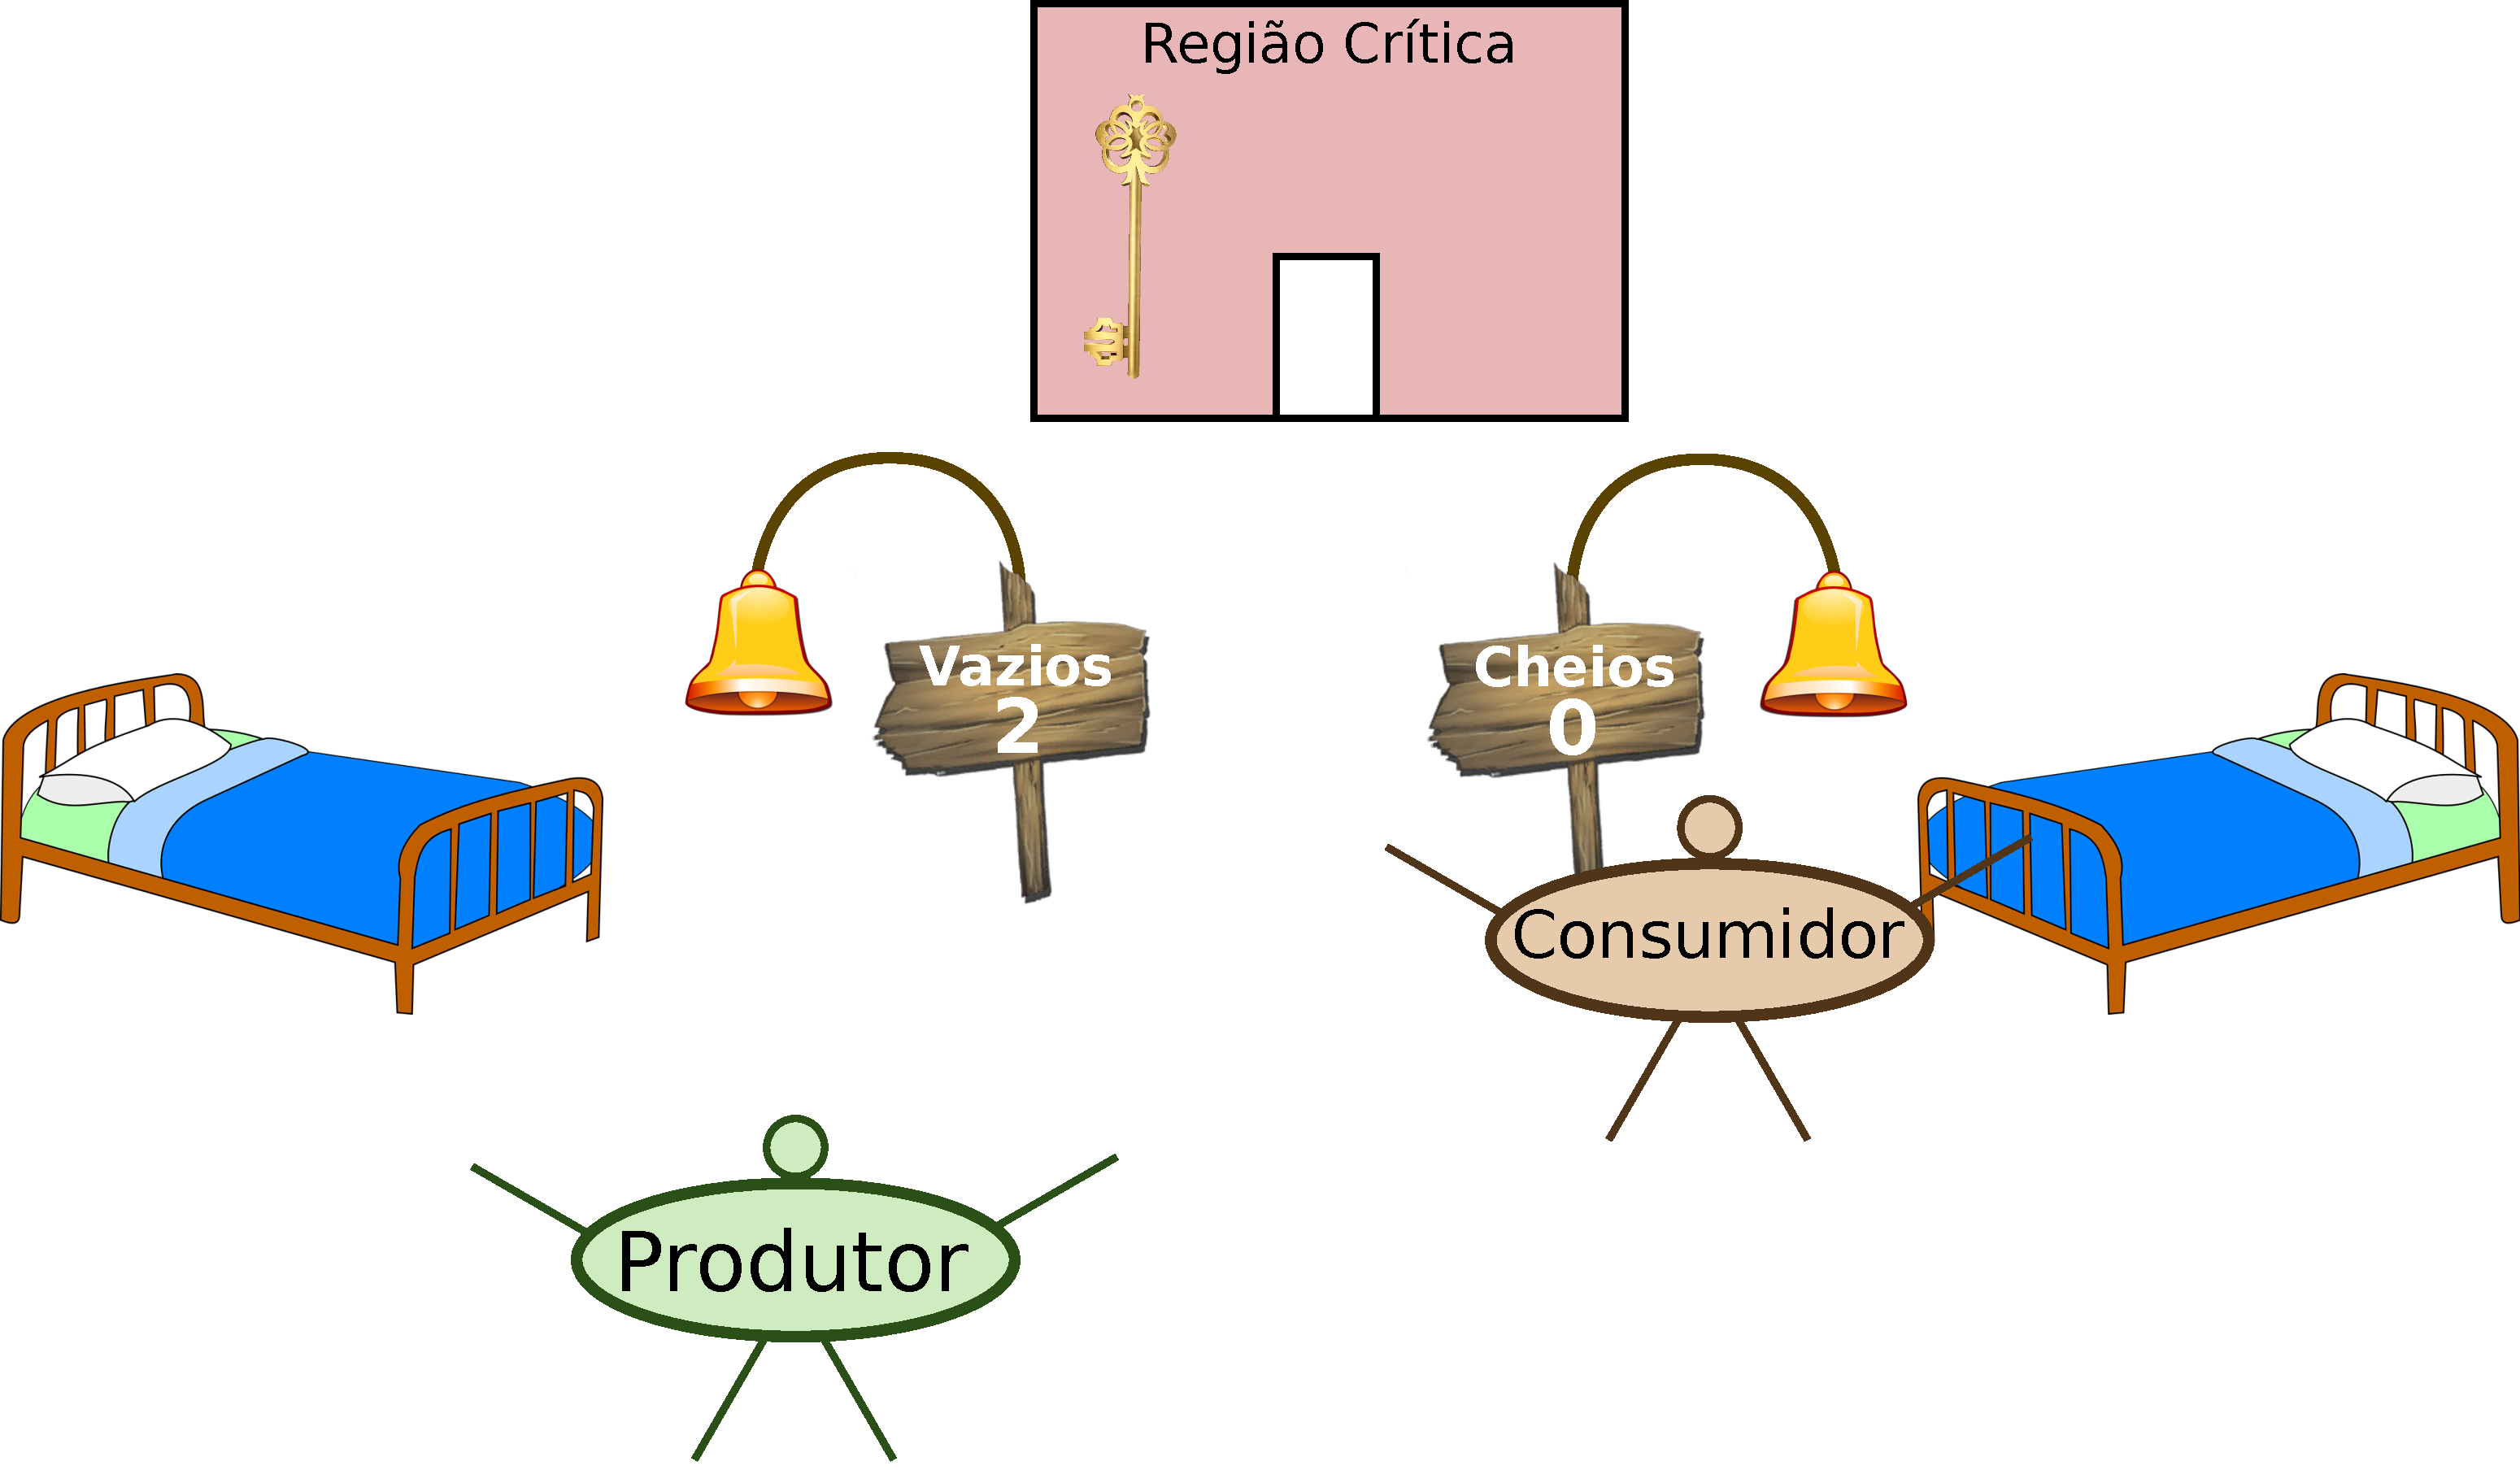
\includegraphics[width=0.9\paperwidth]{resources/semaphore2}}
		\only<3>{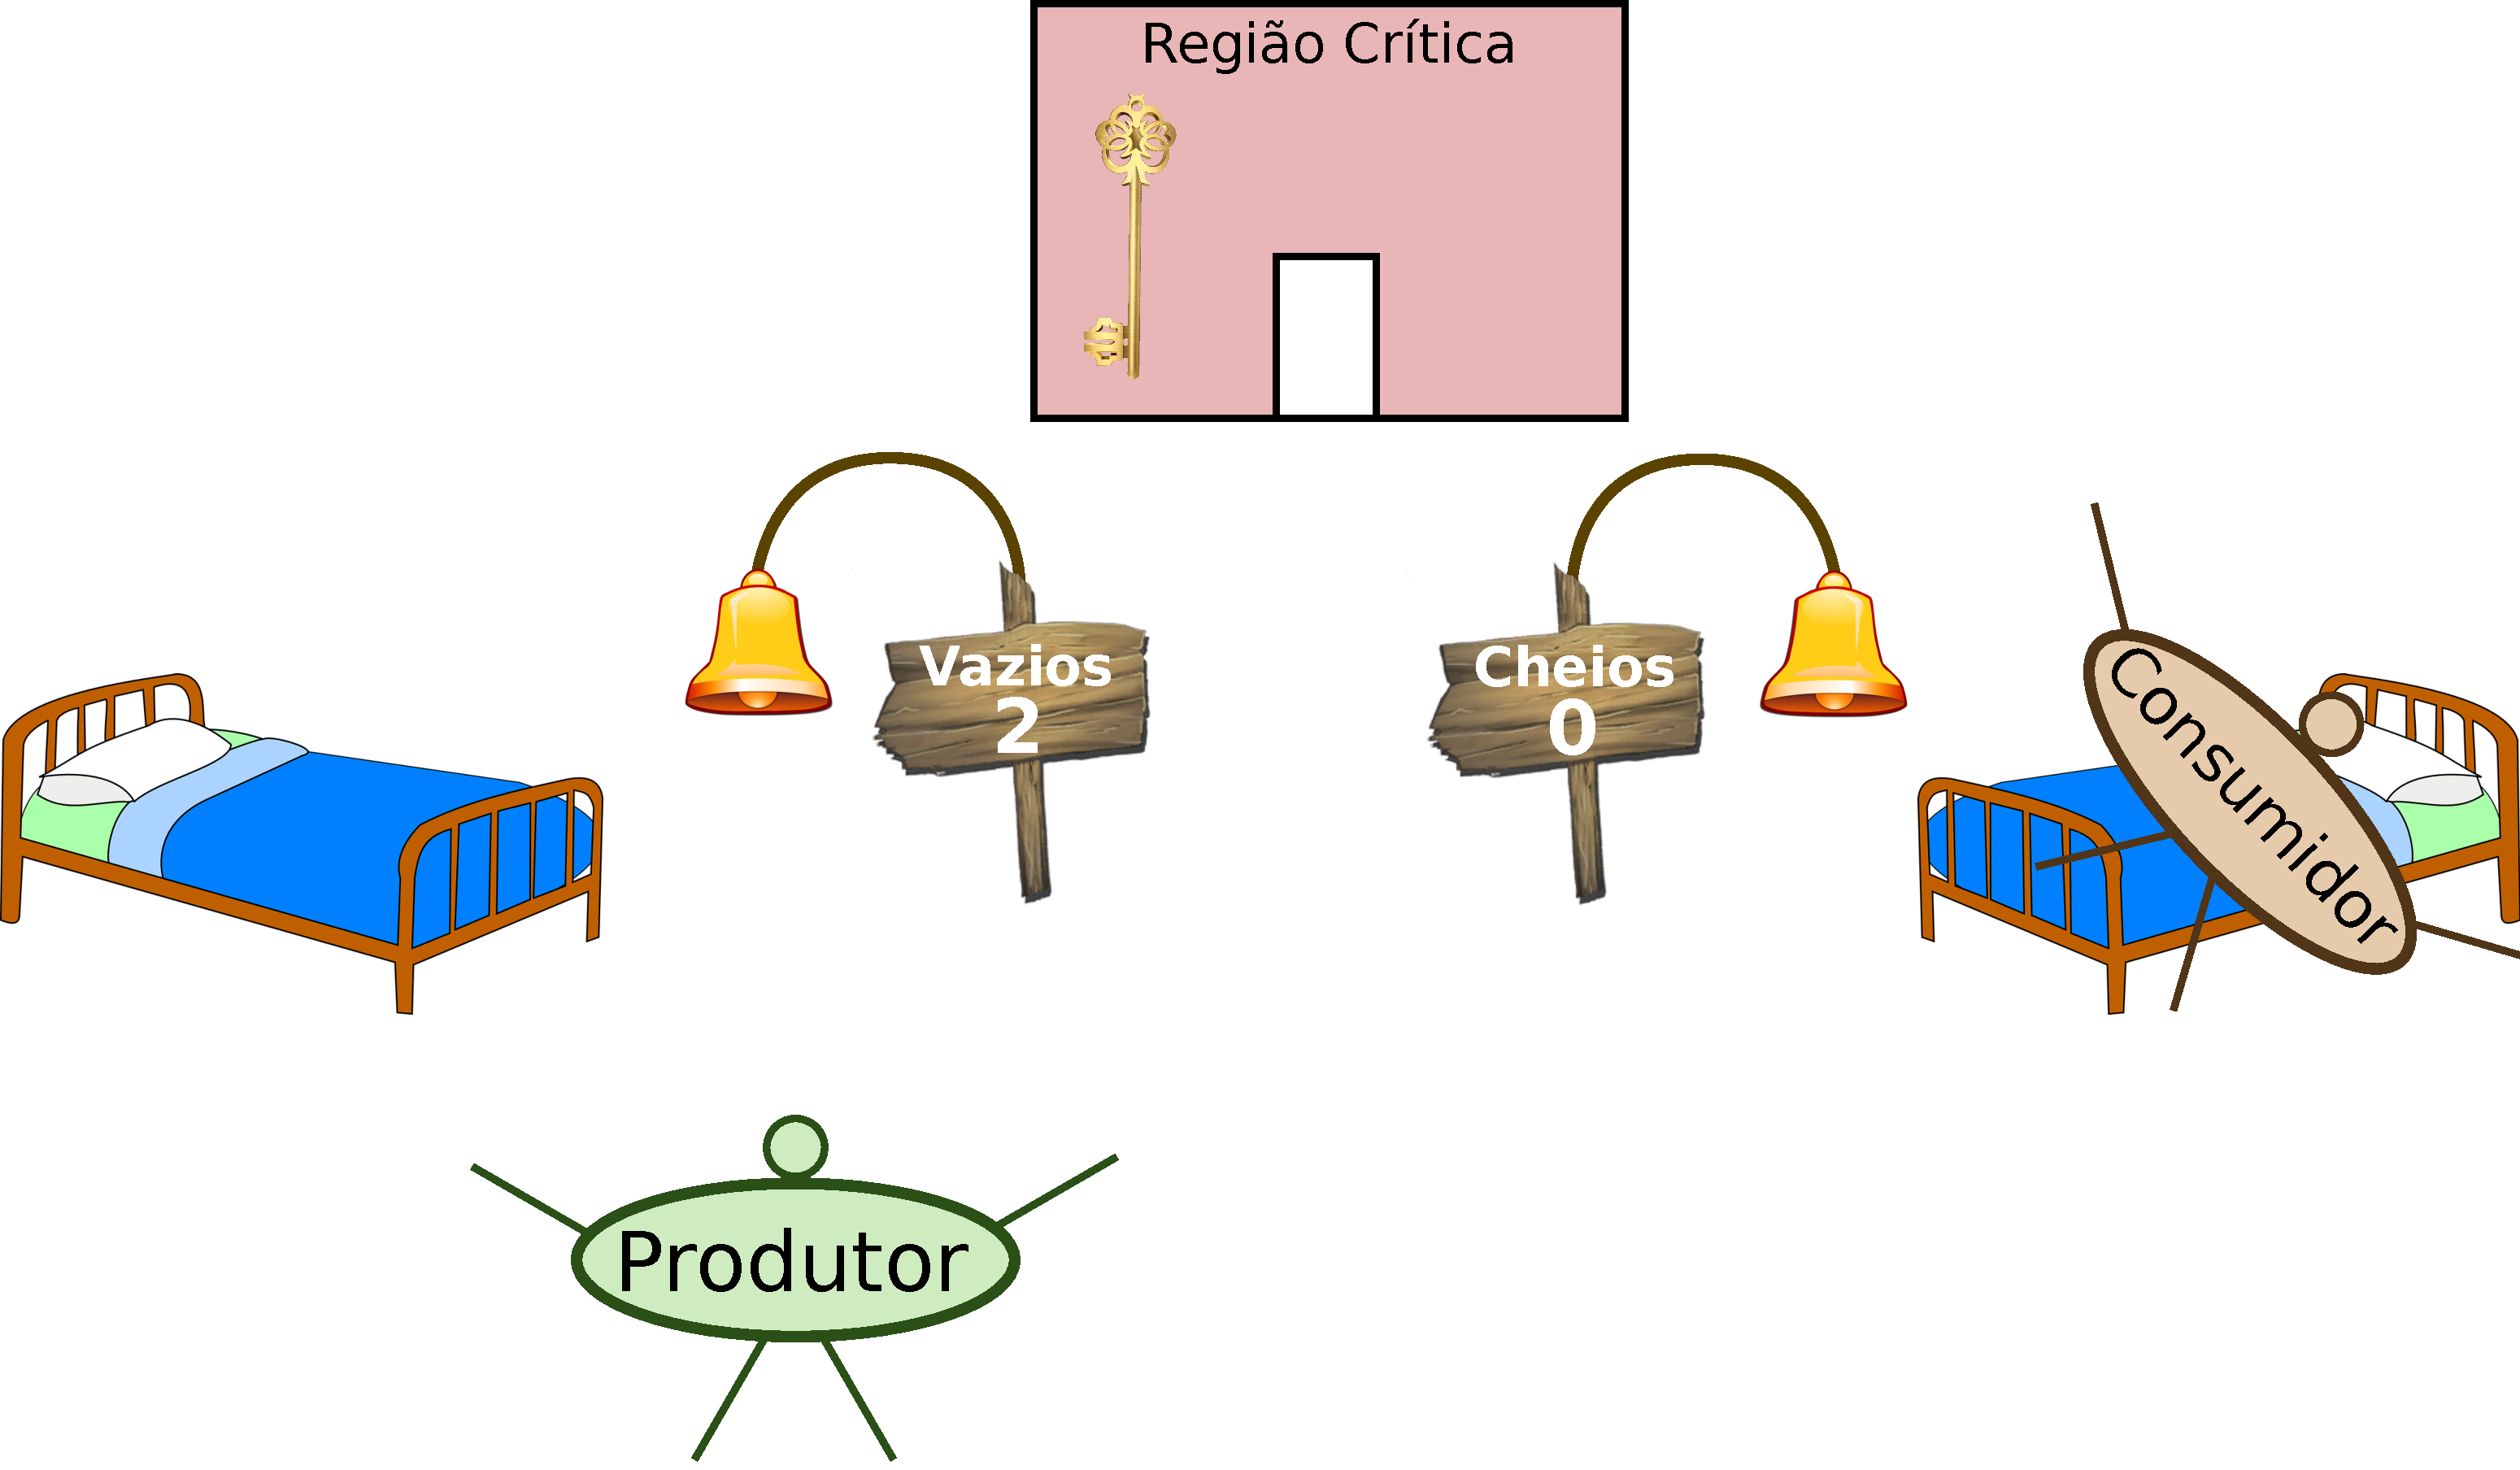
\includegraphics[width=0.9\paperwidth]{resources/semaphore3}}
		\only<4>{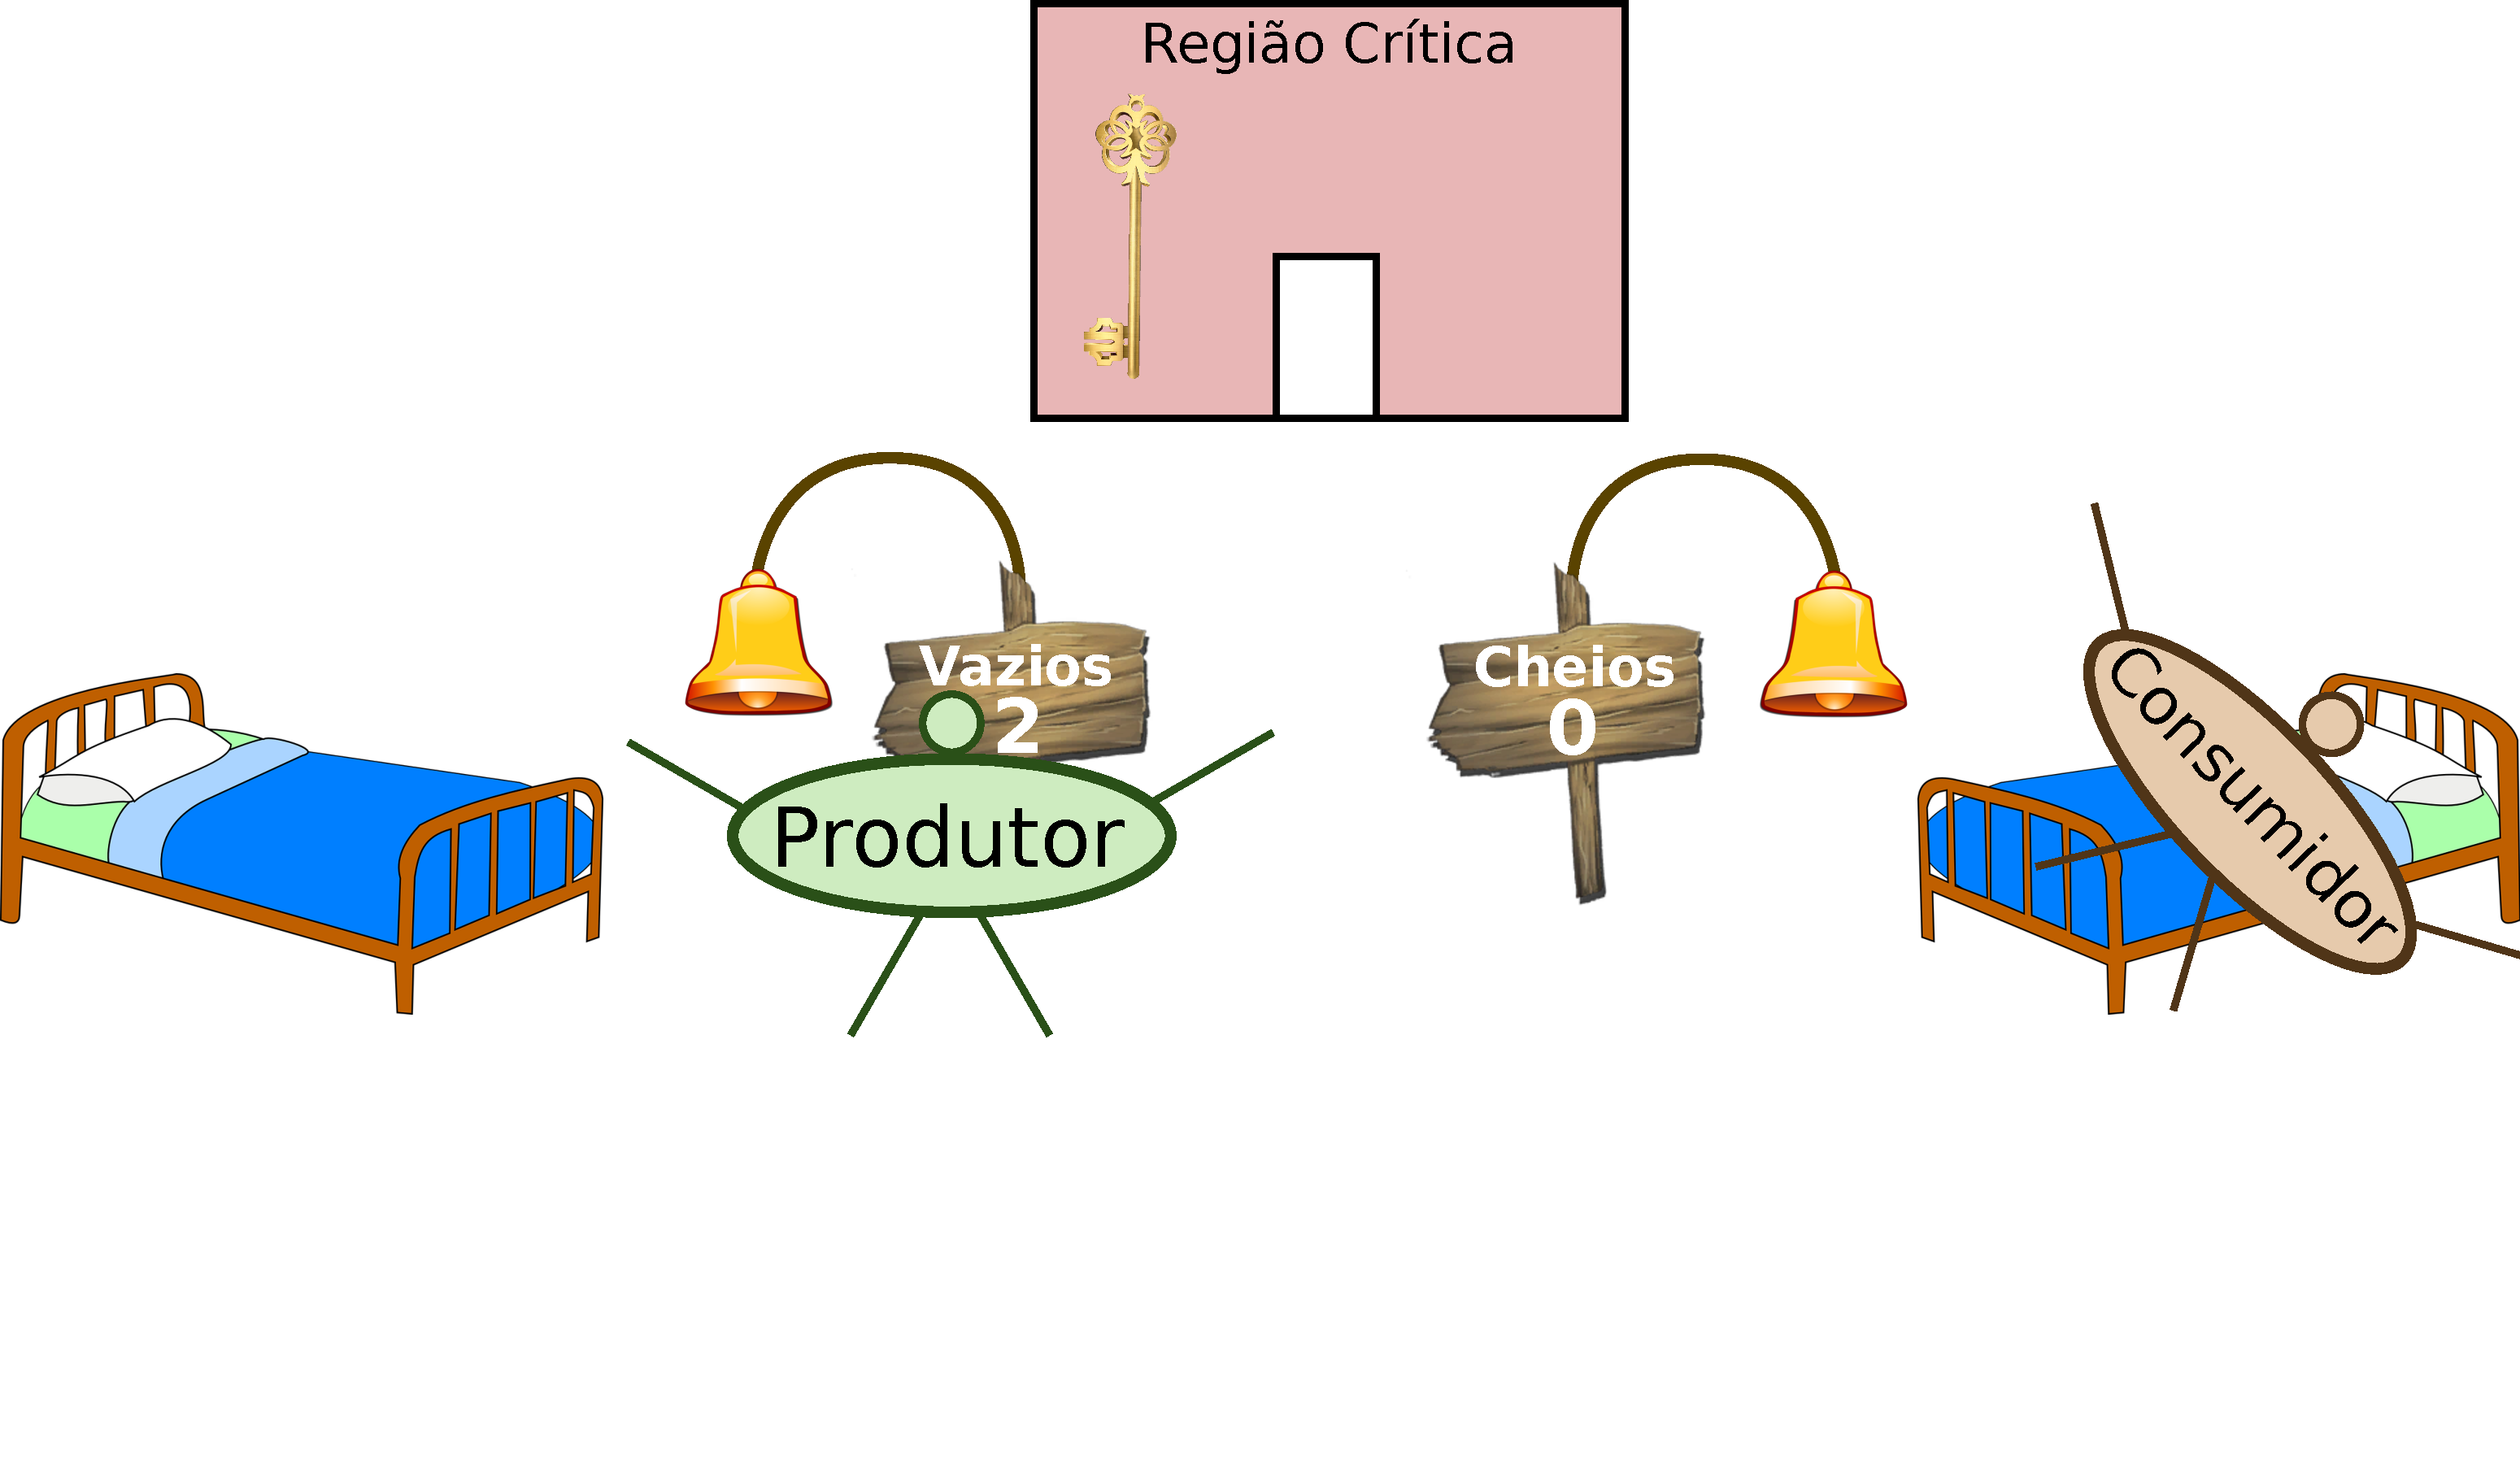
\includegraphics[width=0.9\paperwidth]{resources/semaphore4}}
		\only<5>{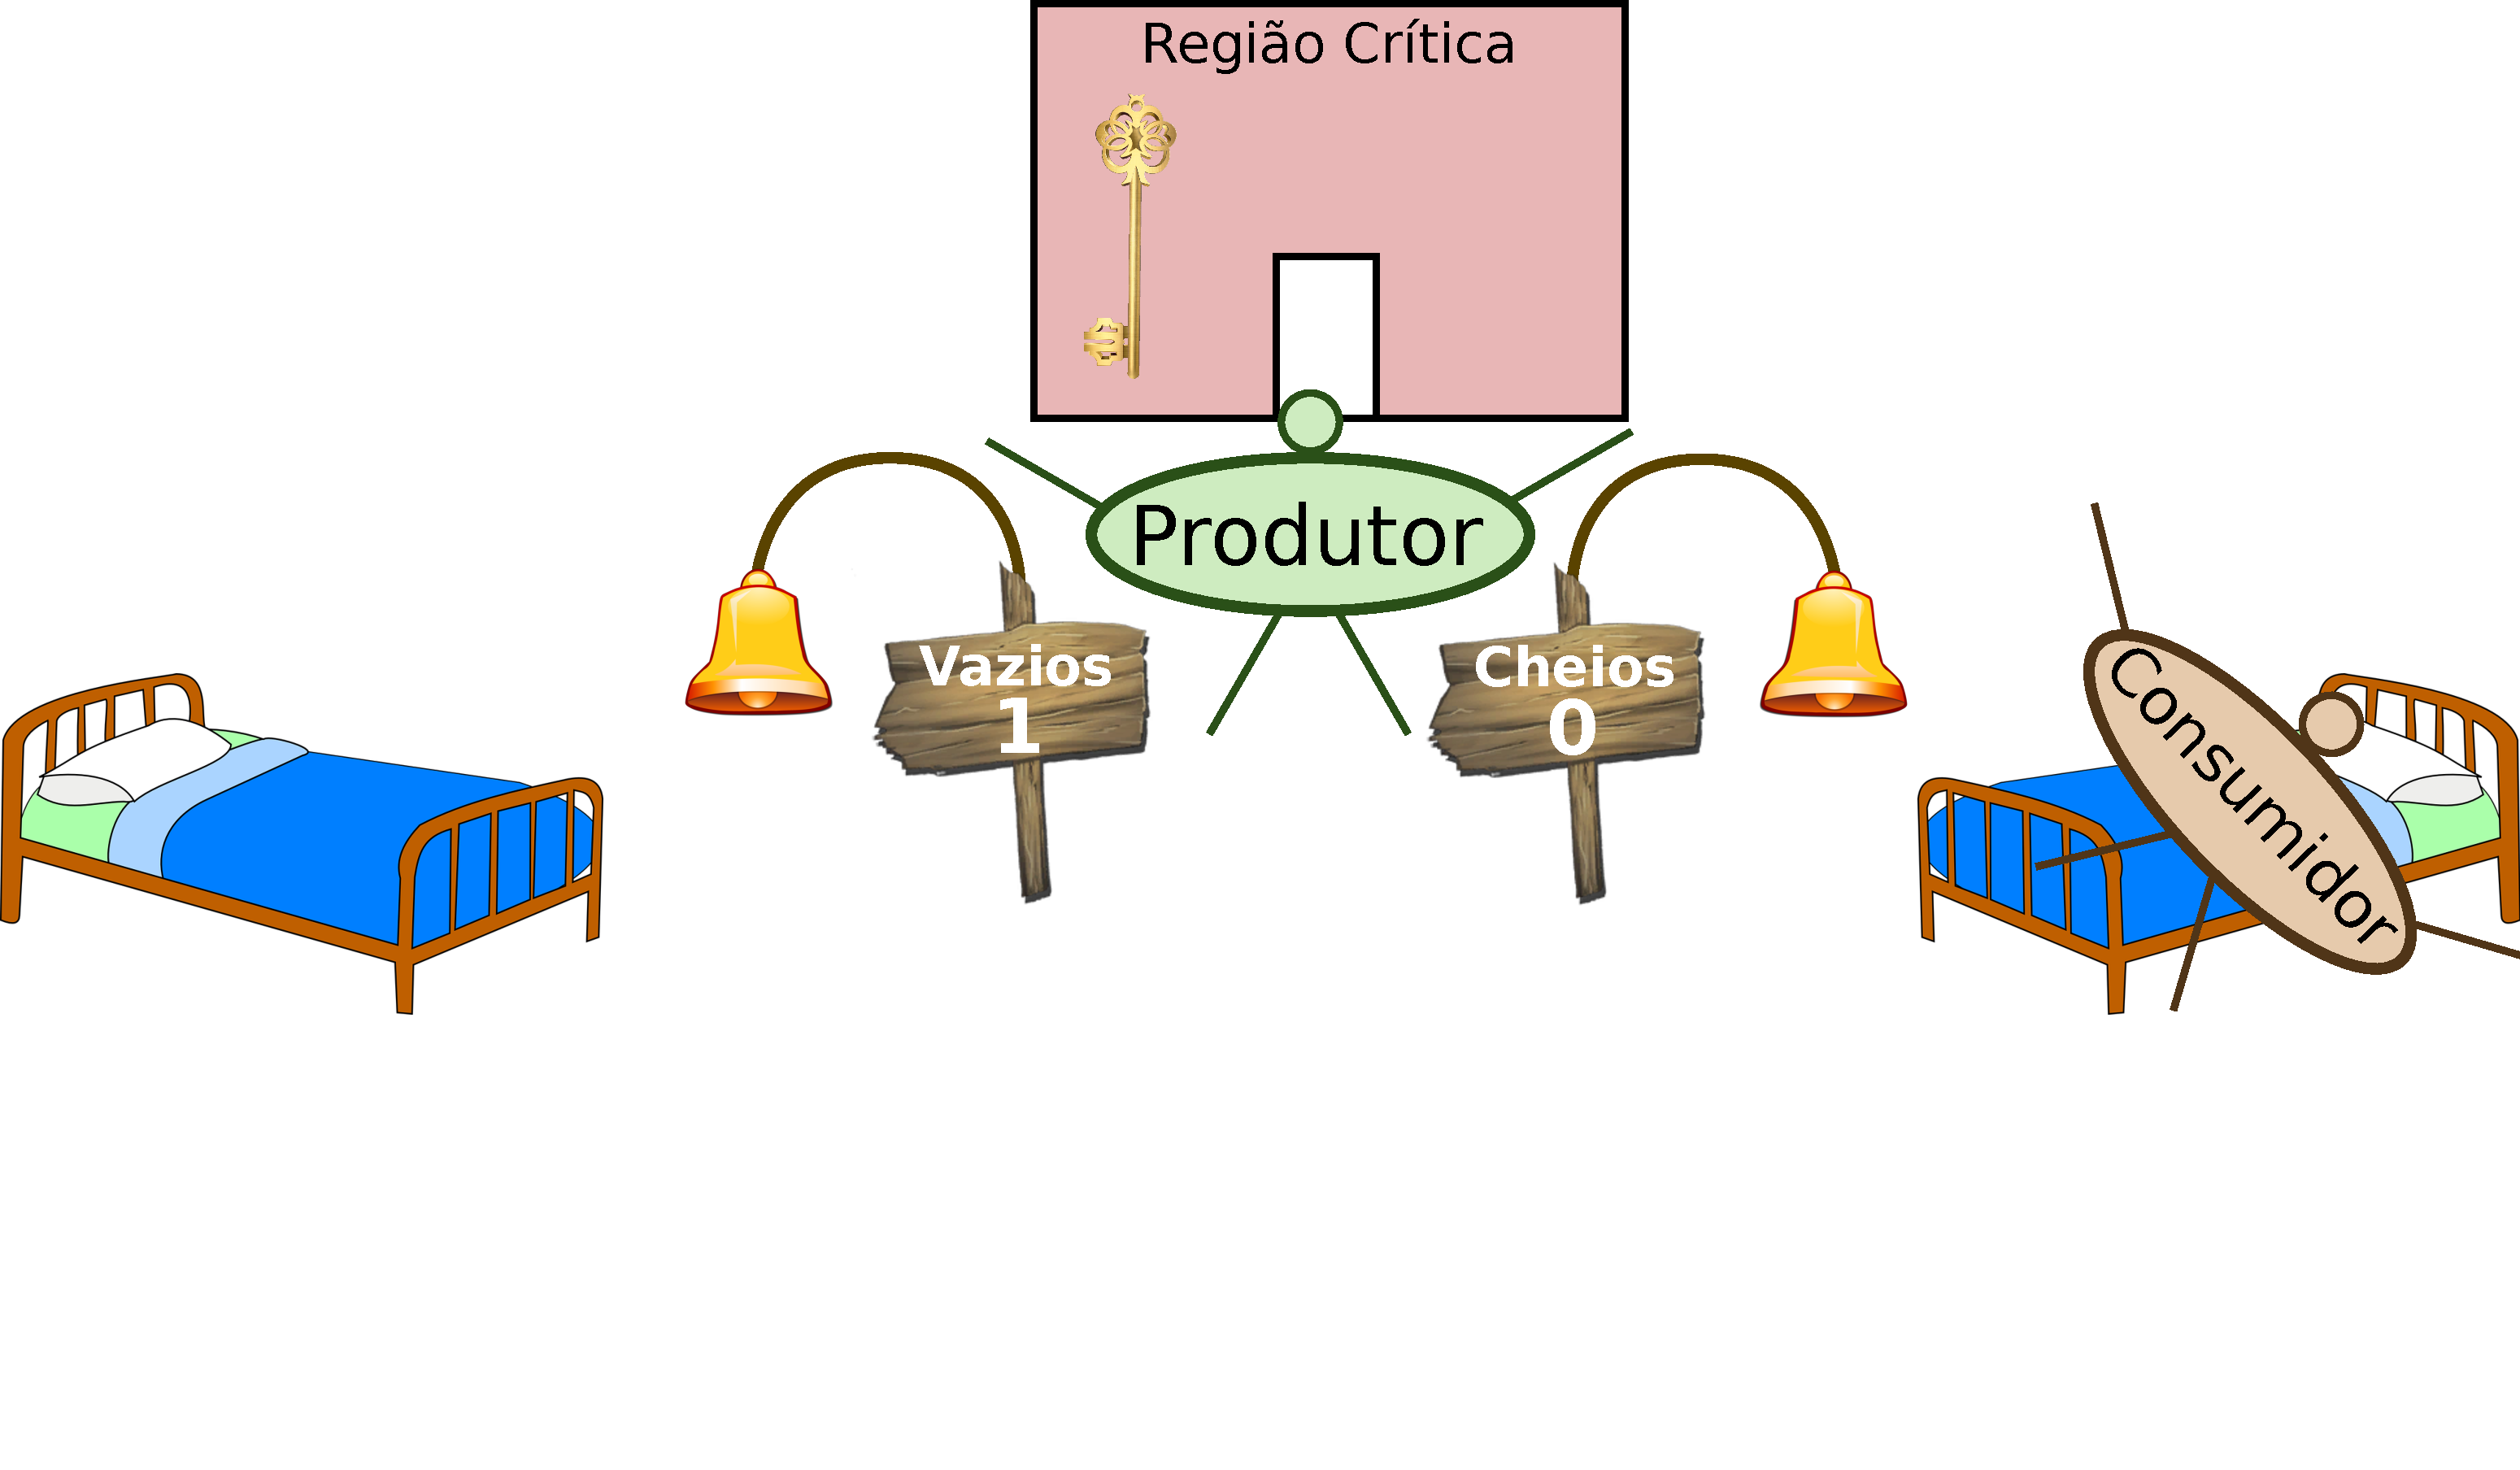
\includegraphics[width=0.9\paperwidth]{resources/semaphore5}}
		\only<6>{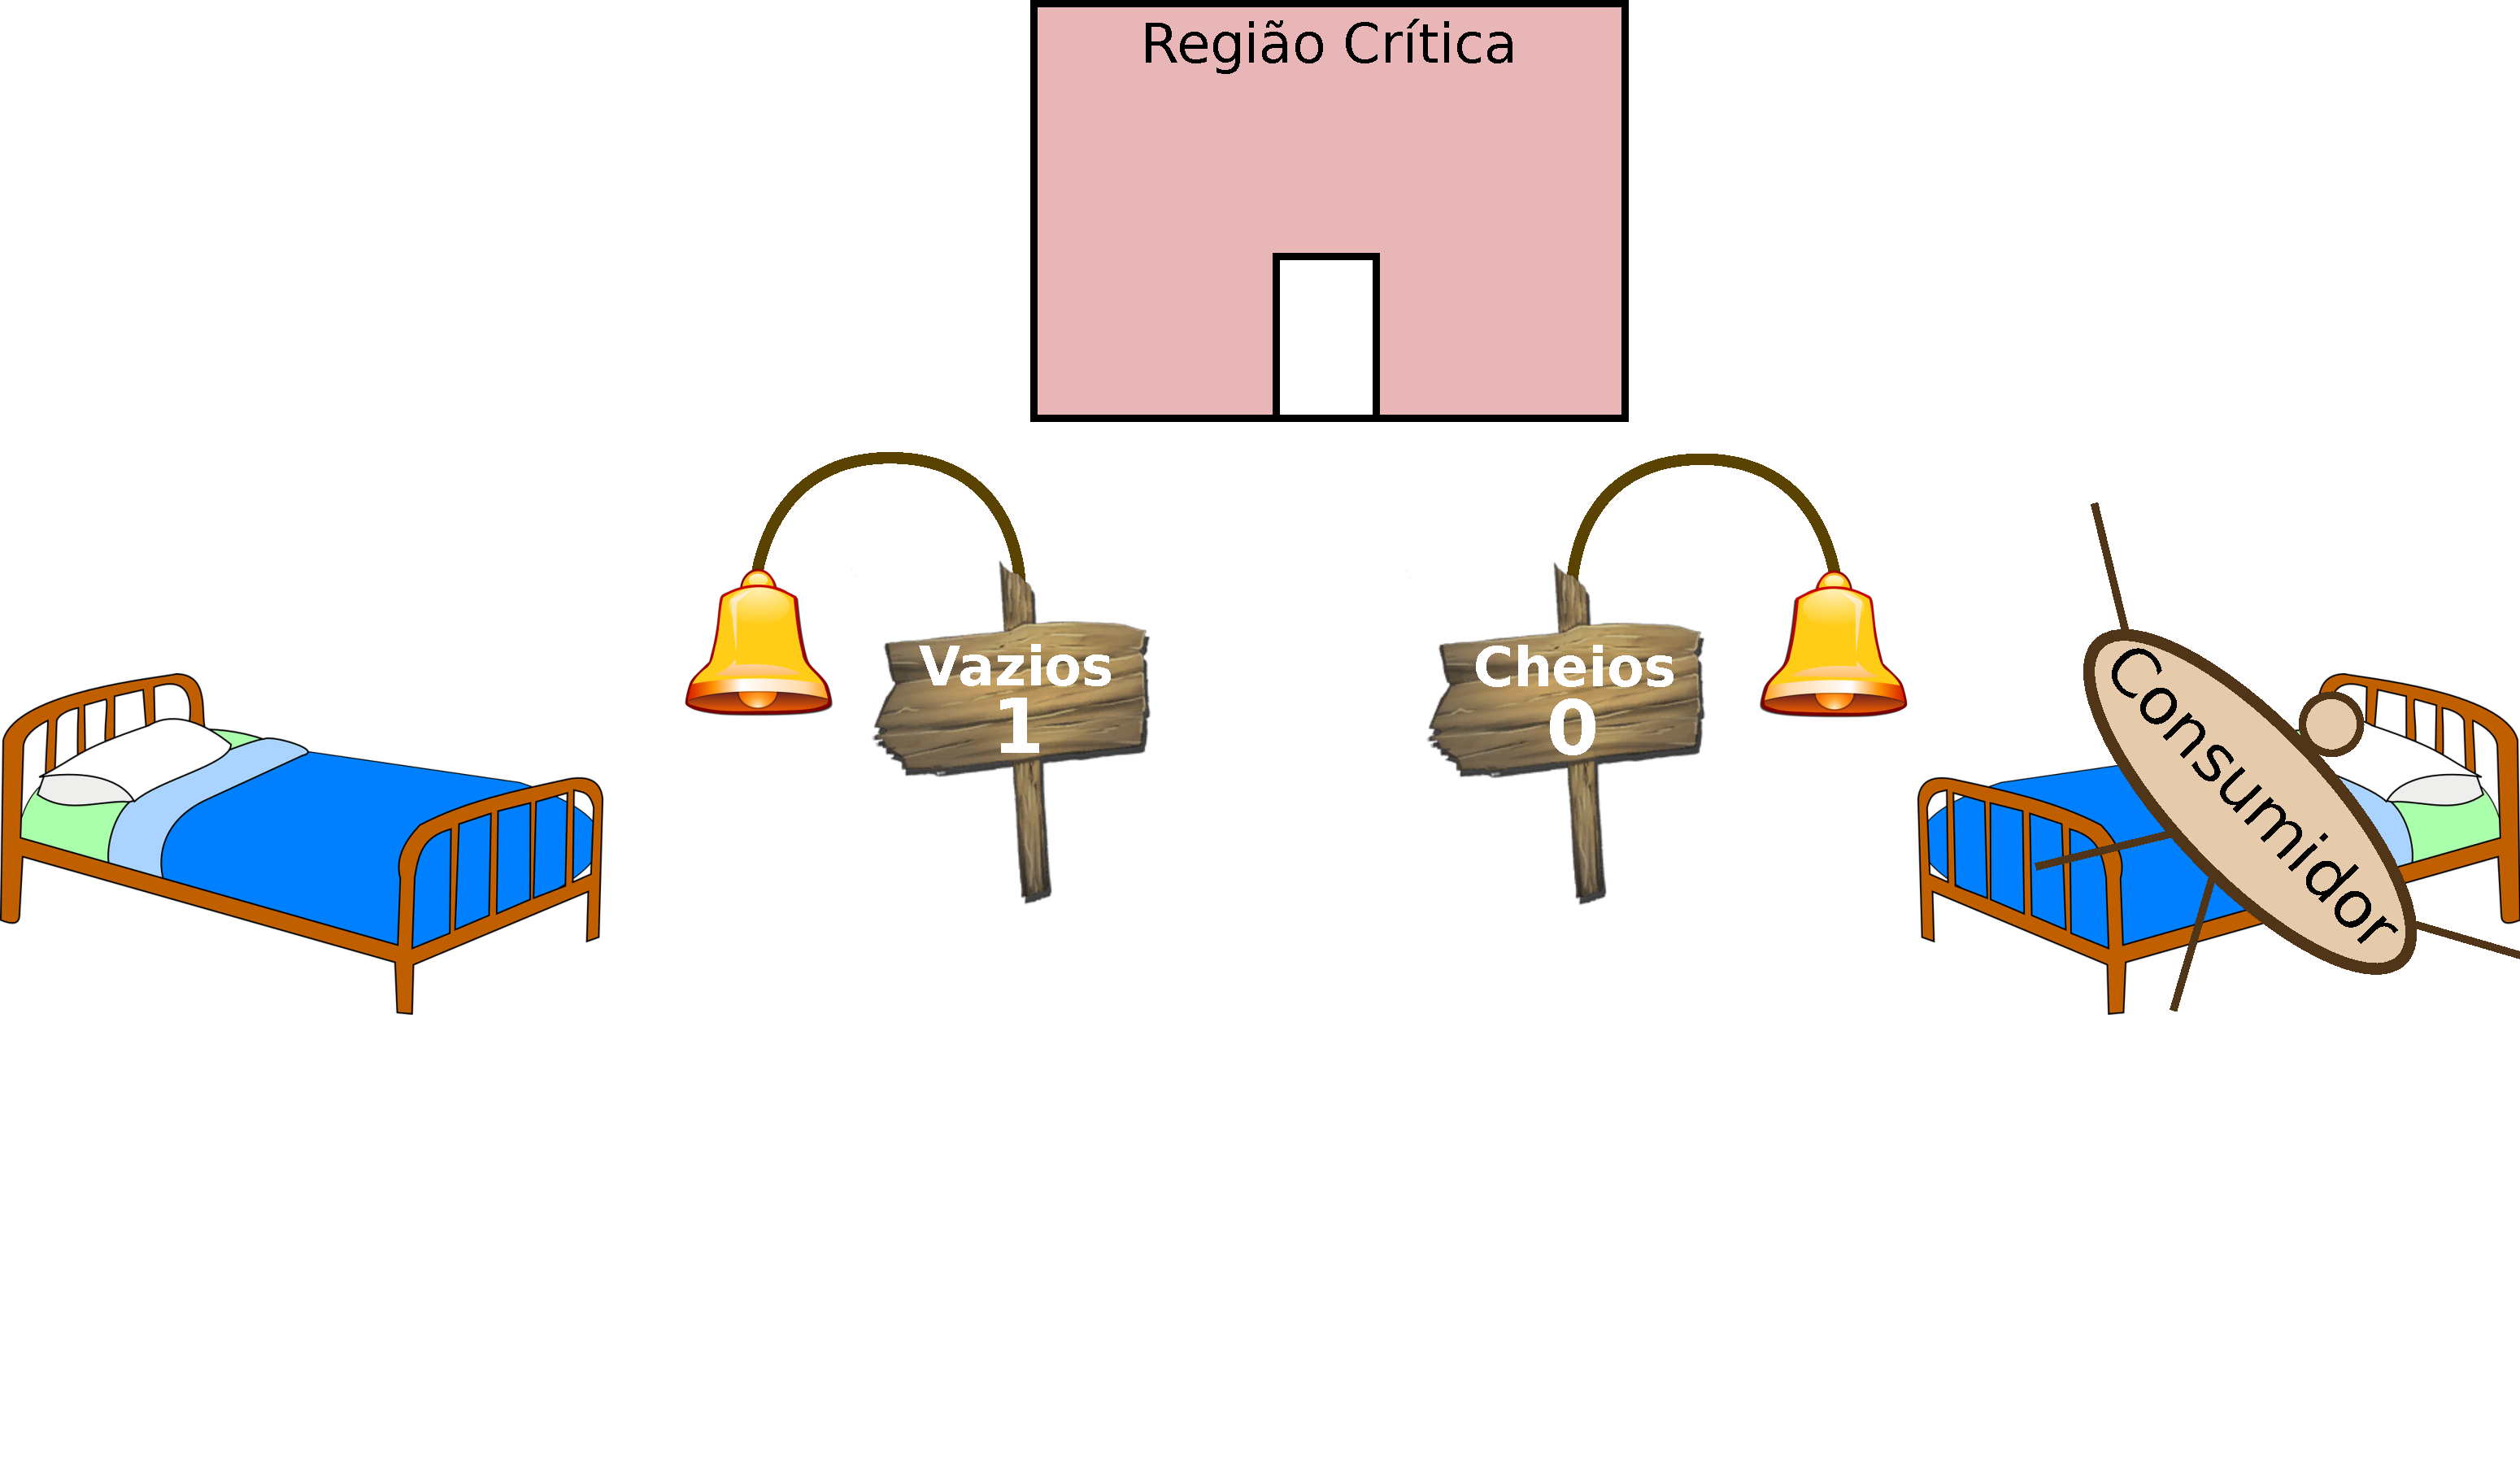
\includegraphics[width=0.9\paperwidth]{resources/semaphore6}}
		\only<7>{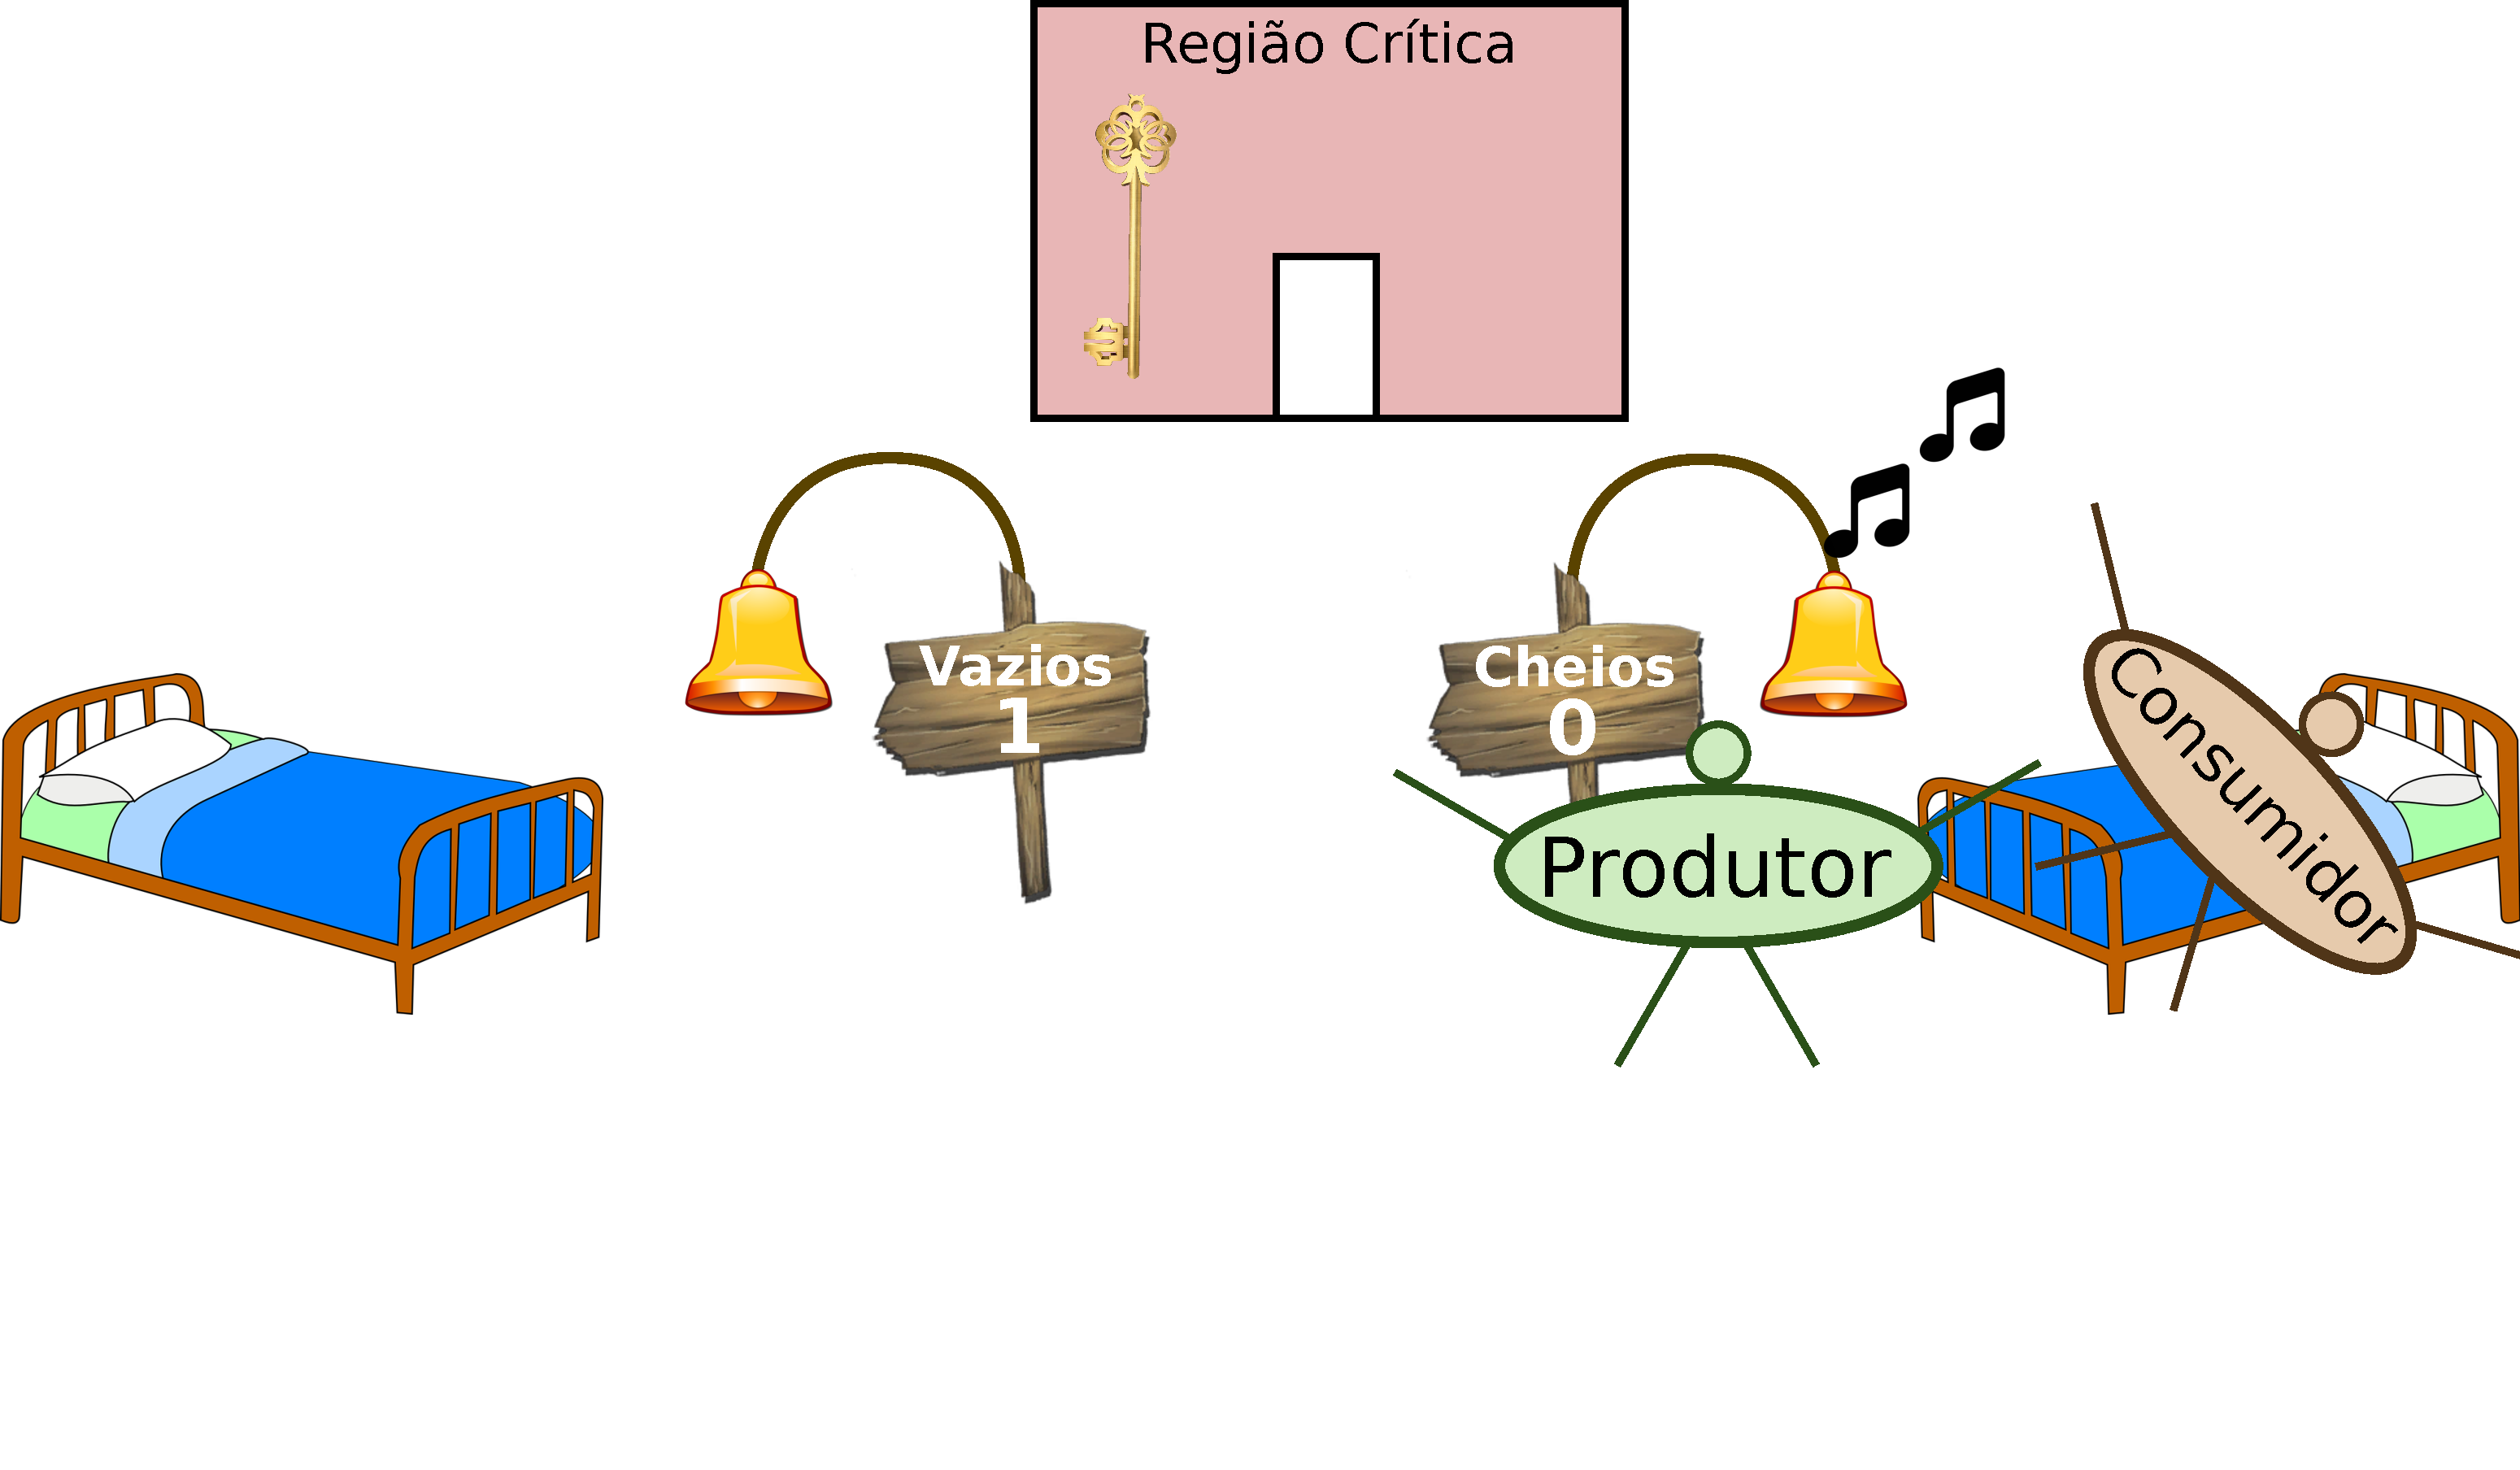
\includegraphics[width=0.9\paperwidth]{resources/semaphore7}}
		\only<8>{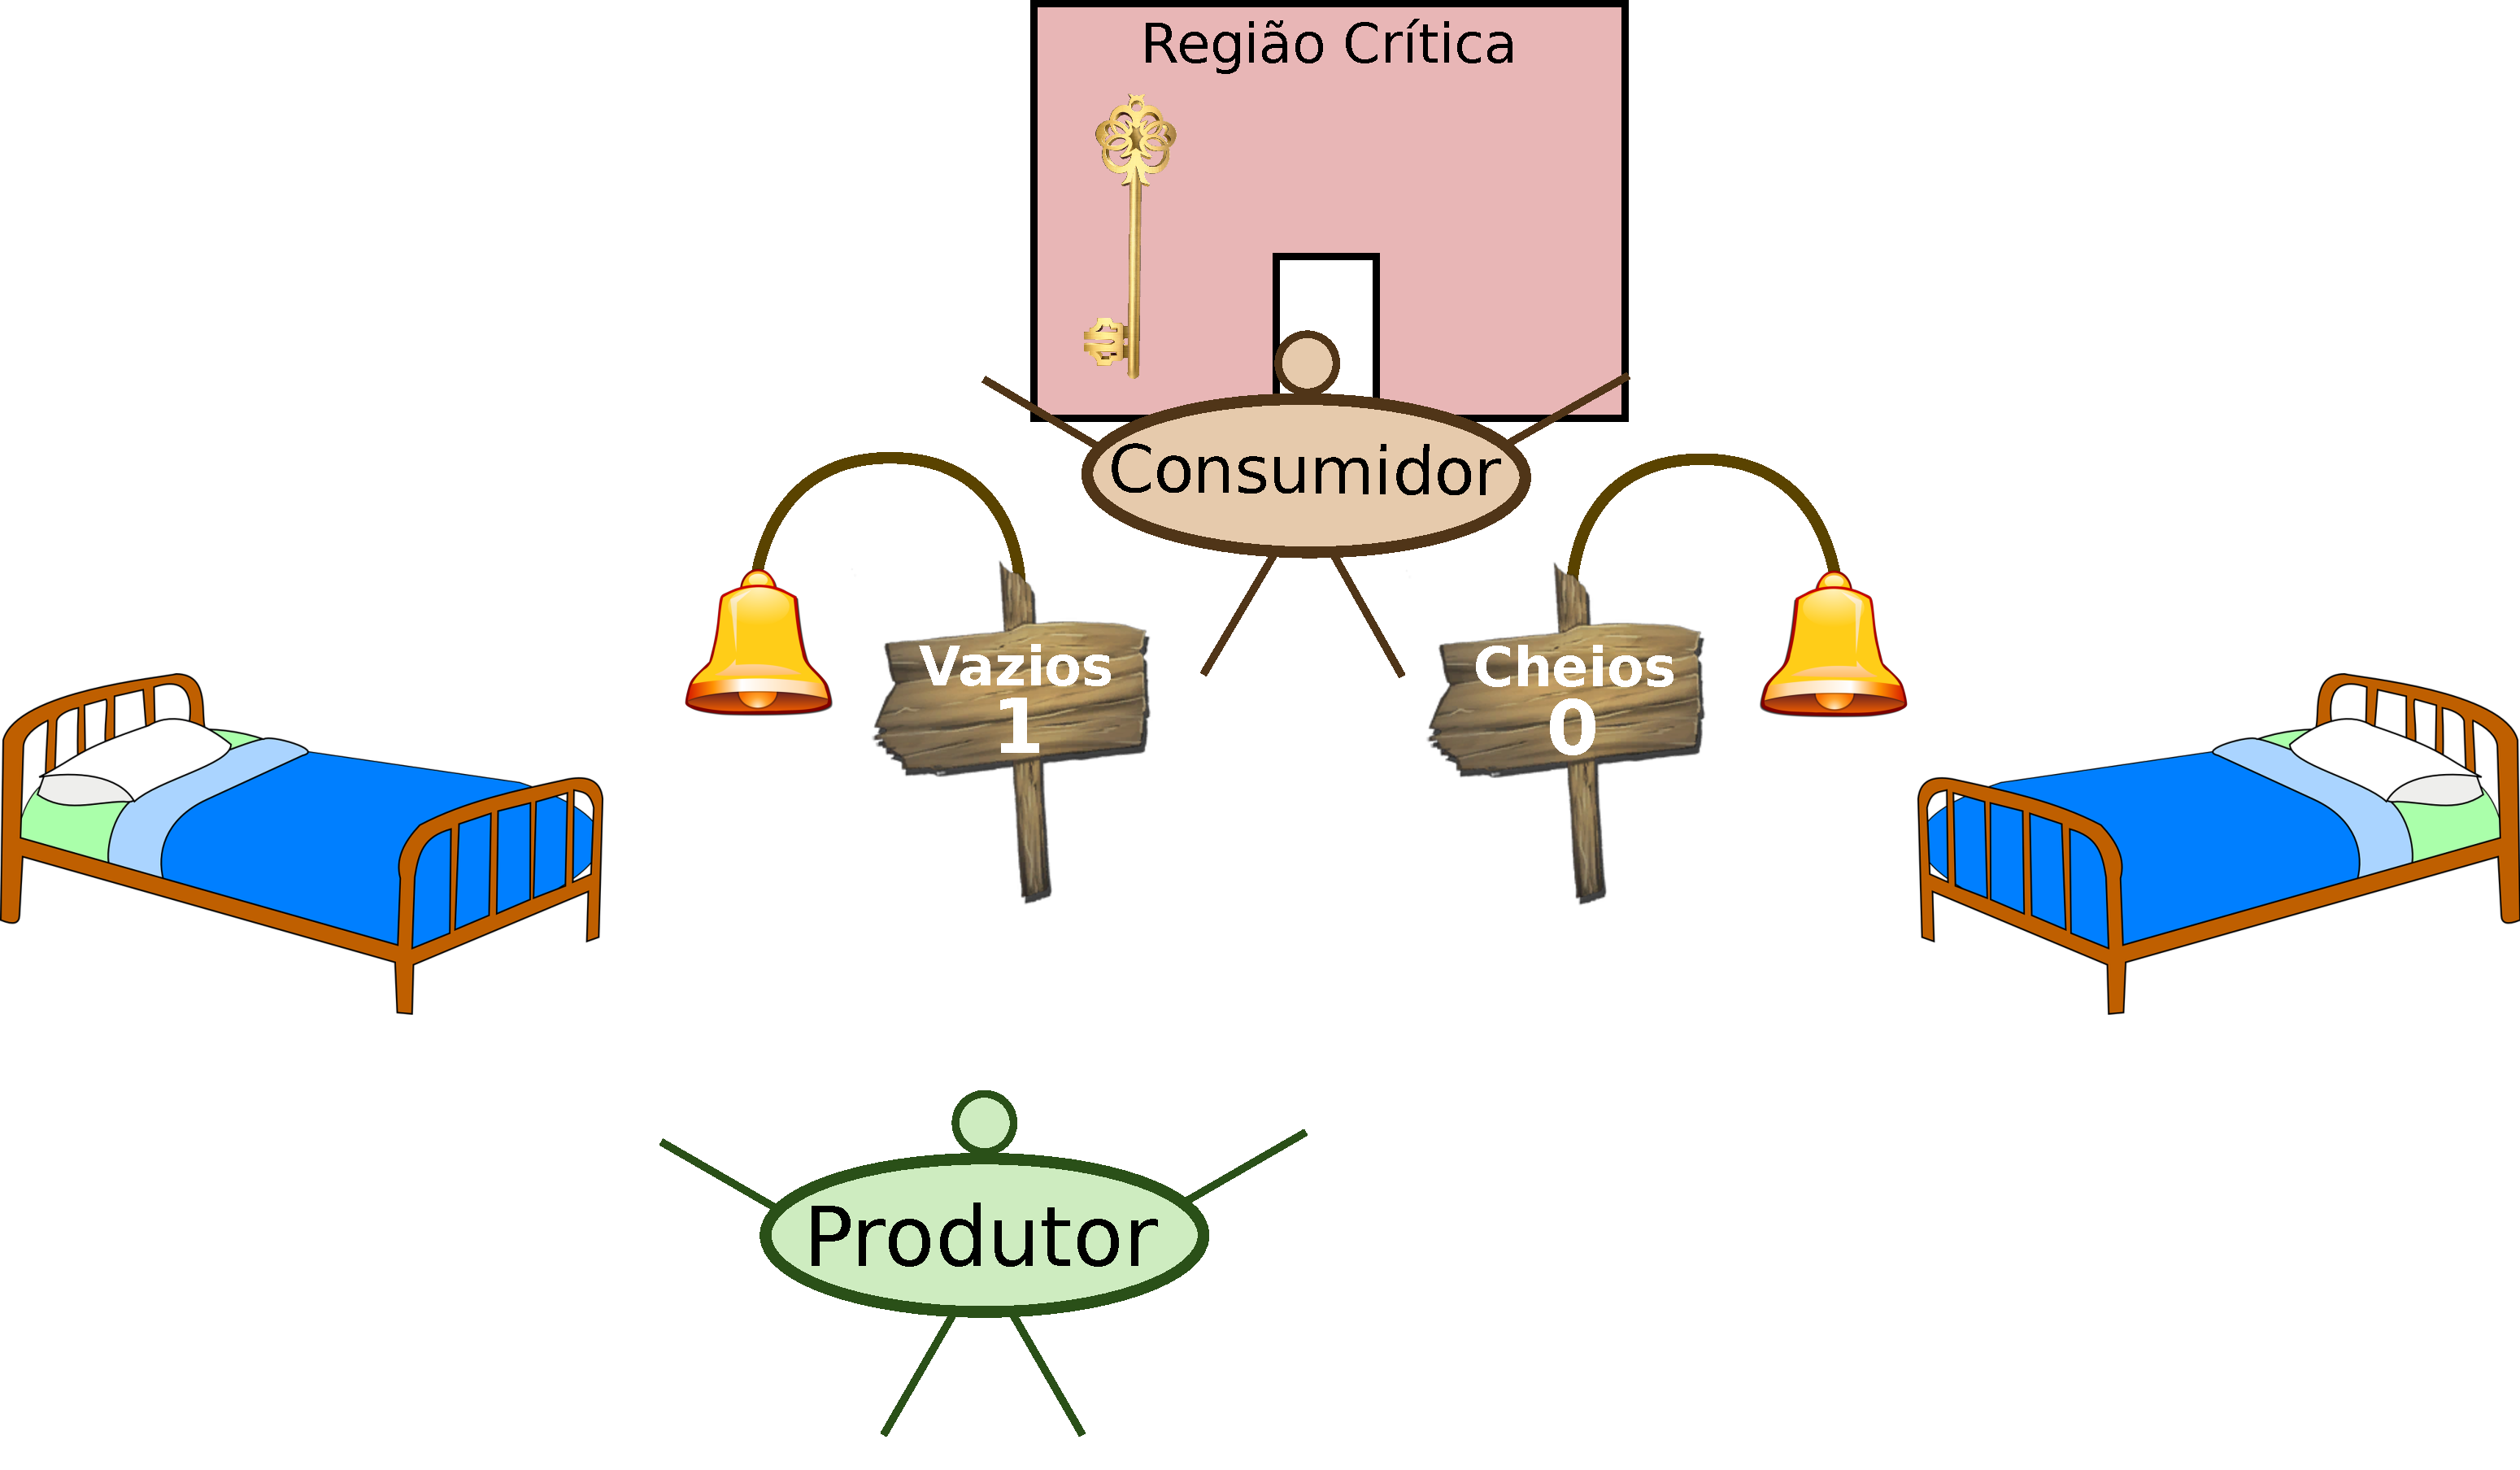
\includegraphics[width=0.9\paperwidth]{resources/semaphore8}}
		\only<9>{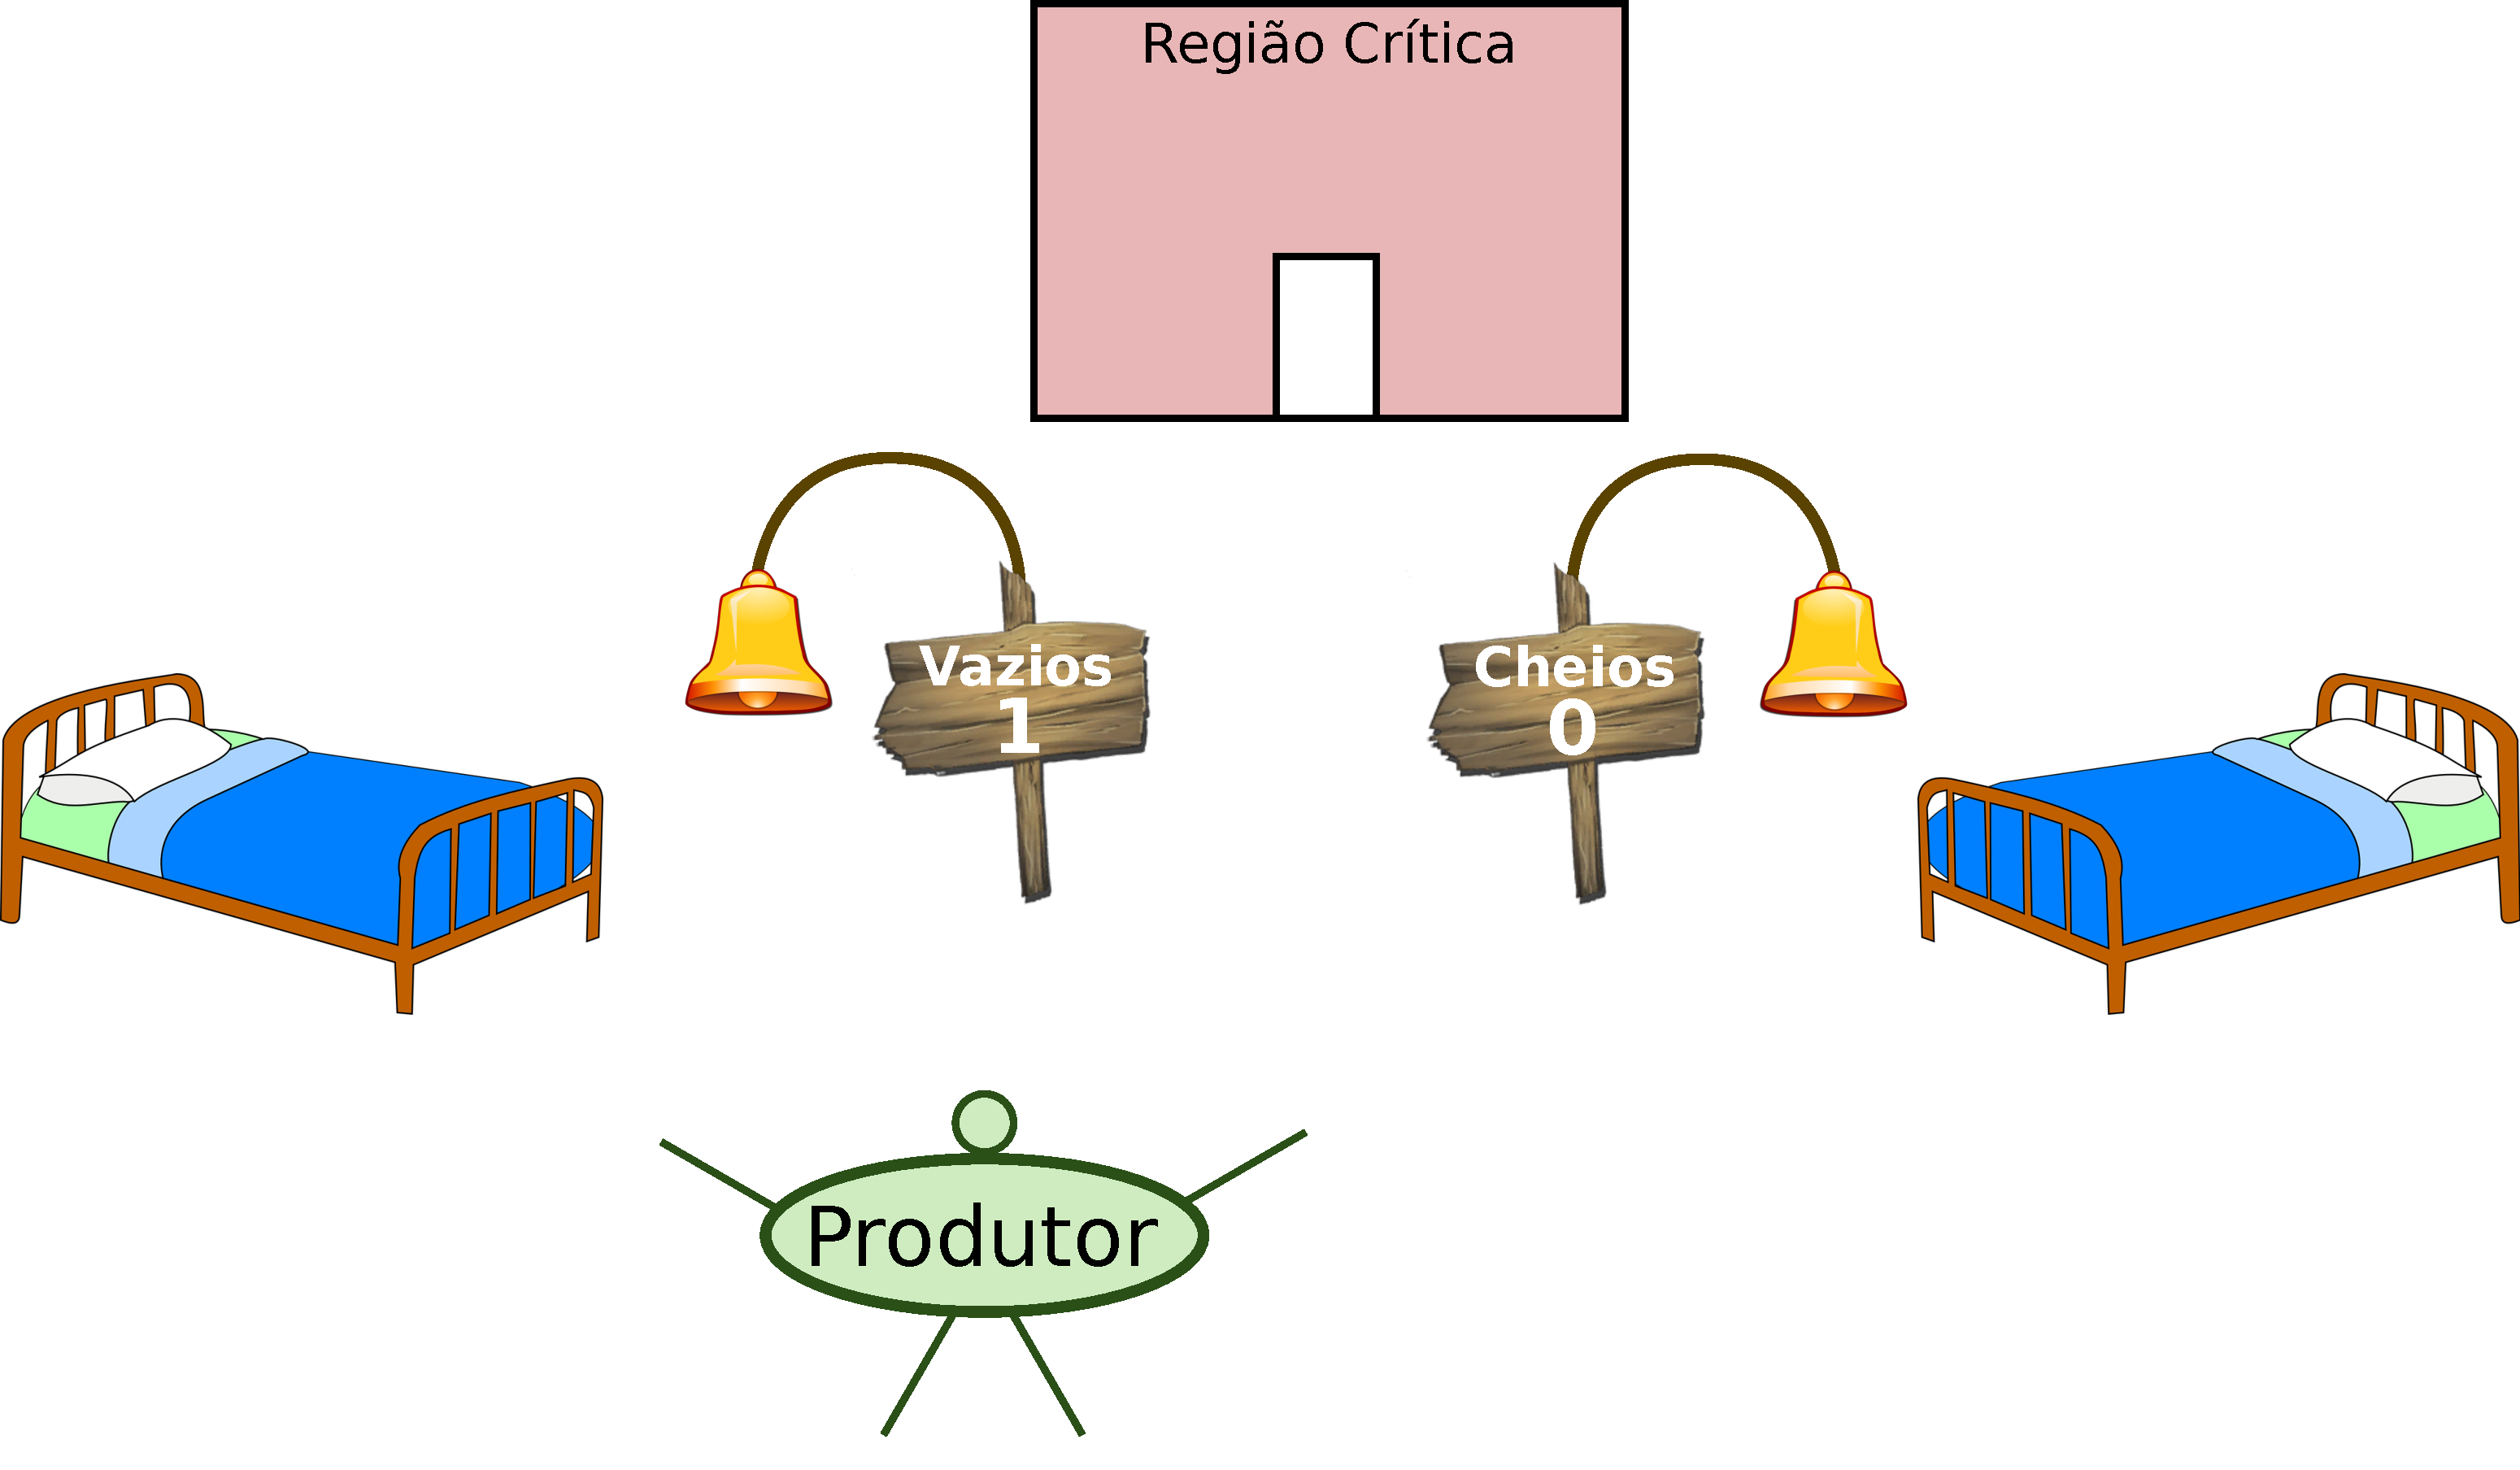
\includegraphics[width=0.9\paperwidth]{resources/semaphore9}}
		\only<10>{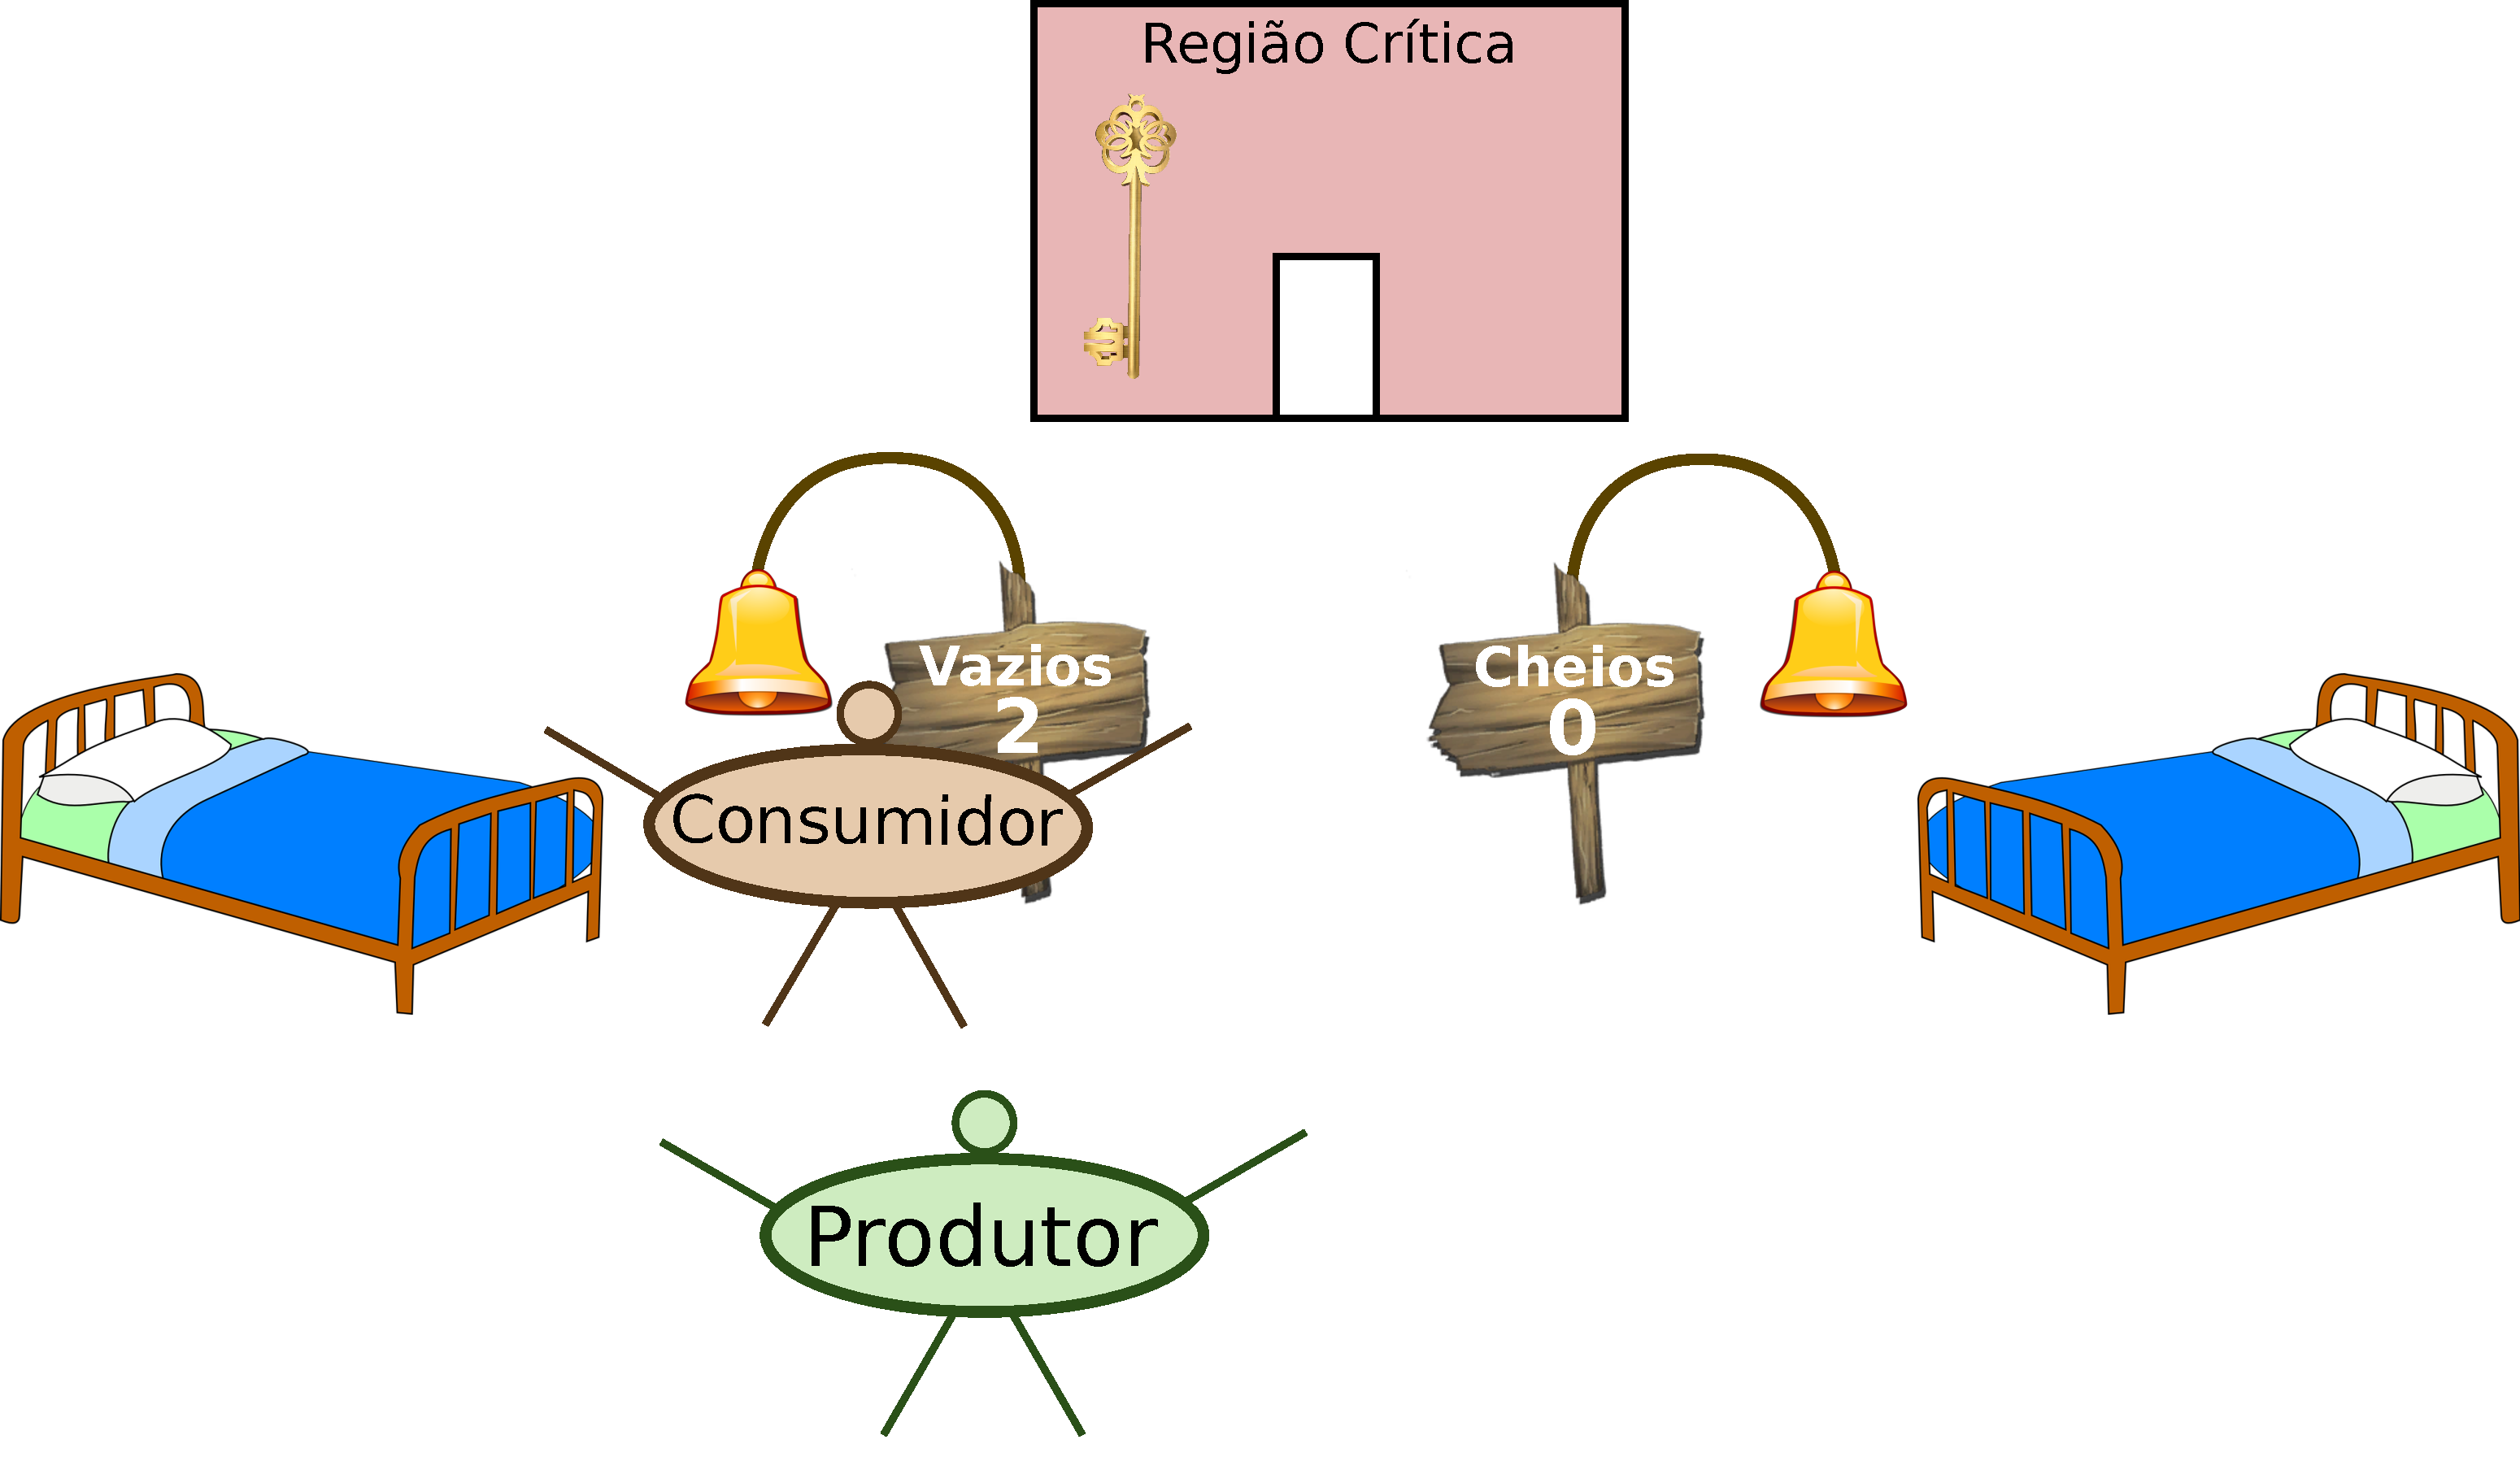
\includegraphics[width=0.9\paperwidth]{resources/semaphore10}}
	\end{figure}
\end{frame}
\begin{frame}{Condições de corrida}
	\framesubtitle{Mutexes}
	\begin{itemize}
		\item Tipo especial de semáforo que só conta até 1
		\item Servem para garantir \textbf{exclusão mútua}
		\item Fáceis e eficientes de implementar (podemos usar \texttt{TSL} ou \texttt{XCHG})
		\item \textbf{Futex:} recurso disponível no Linux semelhante a um mutex, porém mais eficiente, pois evita ao máximo fazer chamadas ao kernel
	\end{itemize}
\end{frame}
\begin{frame}{Condições de corrida}
	\framesubtitle{Mutexes}
	\begin{itemize}
		\item Mutexes estão disponiveis na pthread.
		\item Criar e destruir mutexes:
		\inputminted{c}{resources/pthreadmutexcreate.c}
		\item Travar mutex (down):
		\inputminted{c}{resources/pthreadmutexdown.c}
		\item Destravar mutex (up):
		\inputminted{c}{resources/pthreadmutexup.c}
		\item Tentar travar o mutex:
		\inputminted{c}{resources/pthreadmutextry.c}
	\end{itemize}
\end{frame}
\begin{frame}{Condições de corrida}
	\framesubtitle{Variáveis de condição}
	\begin{itemize}
		\item Outro mecanismo de sincronização oferecido pela pthread
		\item Permitem que um processo bloqueie até que determinada condição seja satisfeita
		\item O processo A \textbf{bloqueia} na variável de condição e fica bloqueado até que o processo B \textbf{sinalize} que ele pode continuar
	\end{itemize}
\end{frame}
\begin{frame}{Condições de corrida}
	\framesubtitle{Variábeis de condição}
	\begin{itemize}
		\item Criar e destruir variáveis de condição:
		\inputminted{c}{resources/pthreadcondcreate.c}
		\item Bloquear em uma variável de condição:
		\inputminted{c}{resources/pthreadcondwait.c}
		\item Sinalizar uma thread para acordá-la:
		\inputminted{c}{resources/pthreadcondsignal.c}
		\item Sinalizar todas as threads para acordá-las:
		\inputminted{c}{resources/pthreadcondbroadcast.c}
	\end{itemize}
\end{frame}
\begin{frame}{Condições de corrida}
	\framesubtitle{Variáveis de condição}
	\begin{itemize}
		\item Variáveis de condição funcionam em conjunto com mutexes
		\item Para fazer \texttt{wait} em uma variável de condição, é preciso ter a posse do mutex
		\item O \texttt{wait}, então, libera a posse do mutex
		\item Quando \texttt{signal} é chamado, a thread é acordada e recupera a posse do mutex
	\end{itemize}
\end{frame}
\begin{frame}{Condições de corrida}
	\begin{figure}
		\only<1>{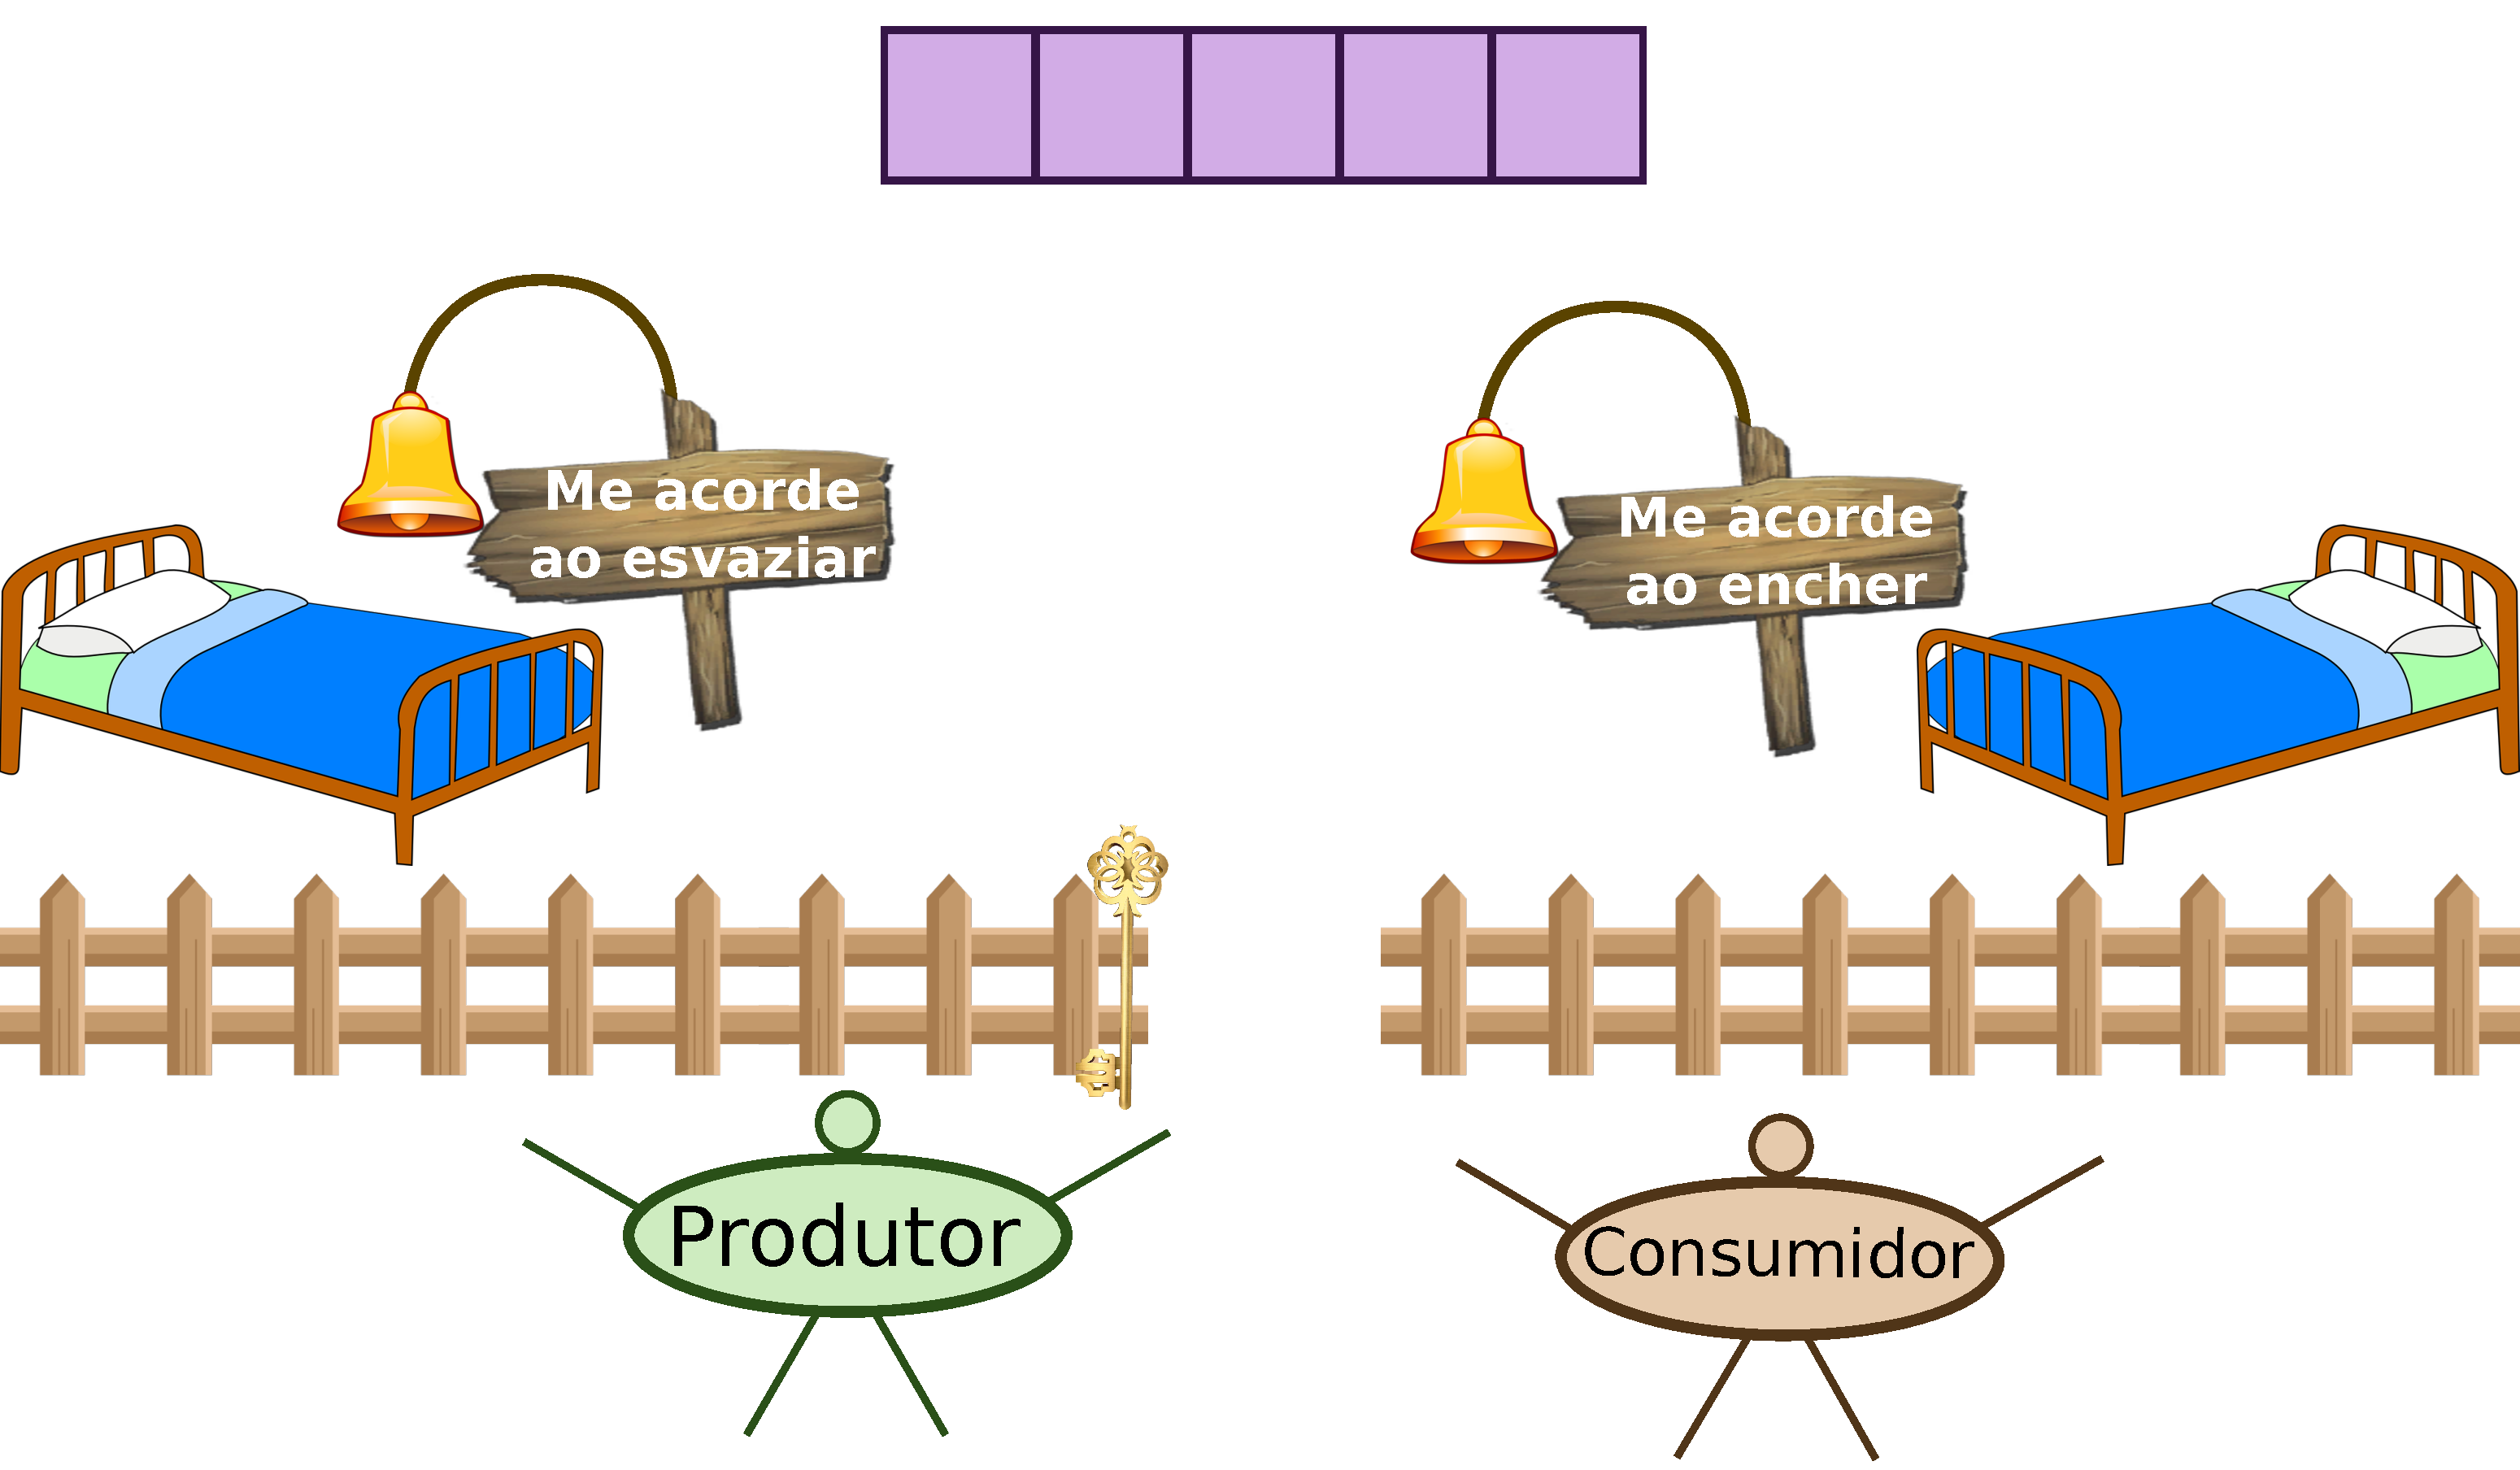
\includegraphics[width=0.9\paperwidth]{resources/cond1}}
		\only<2>{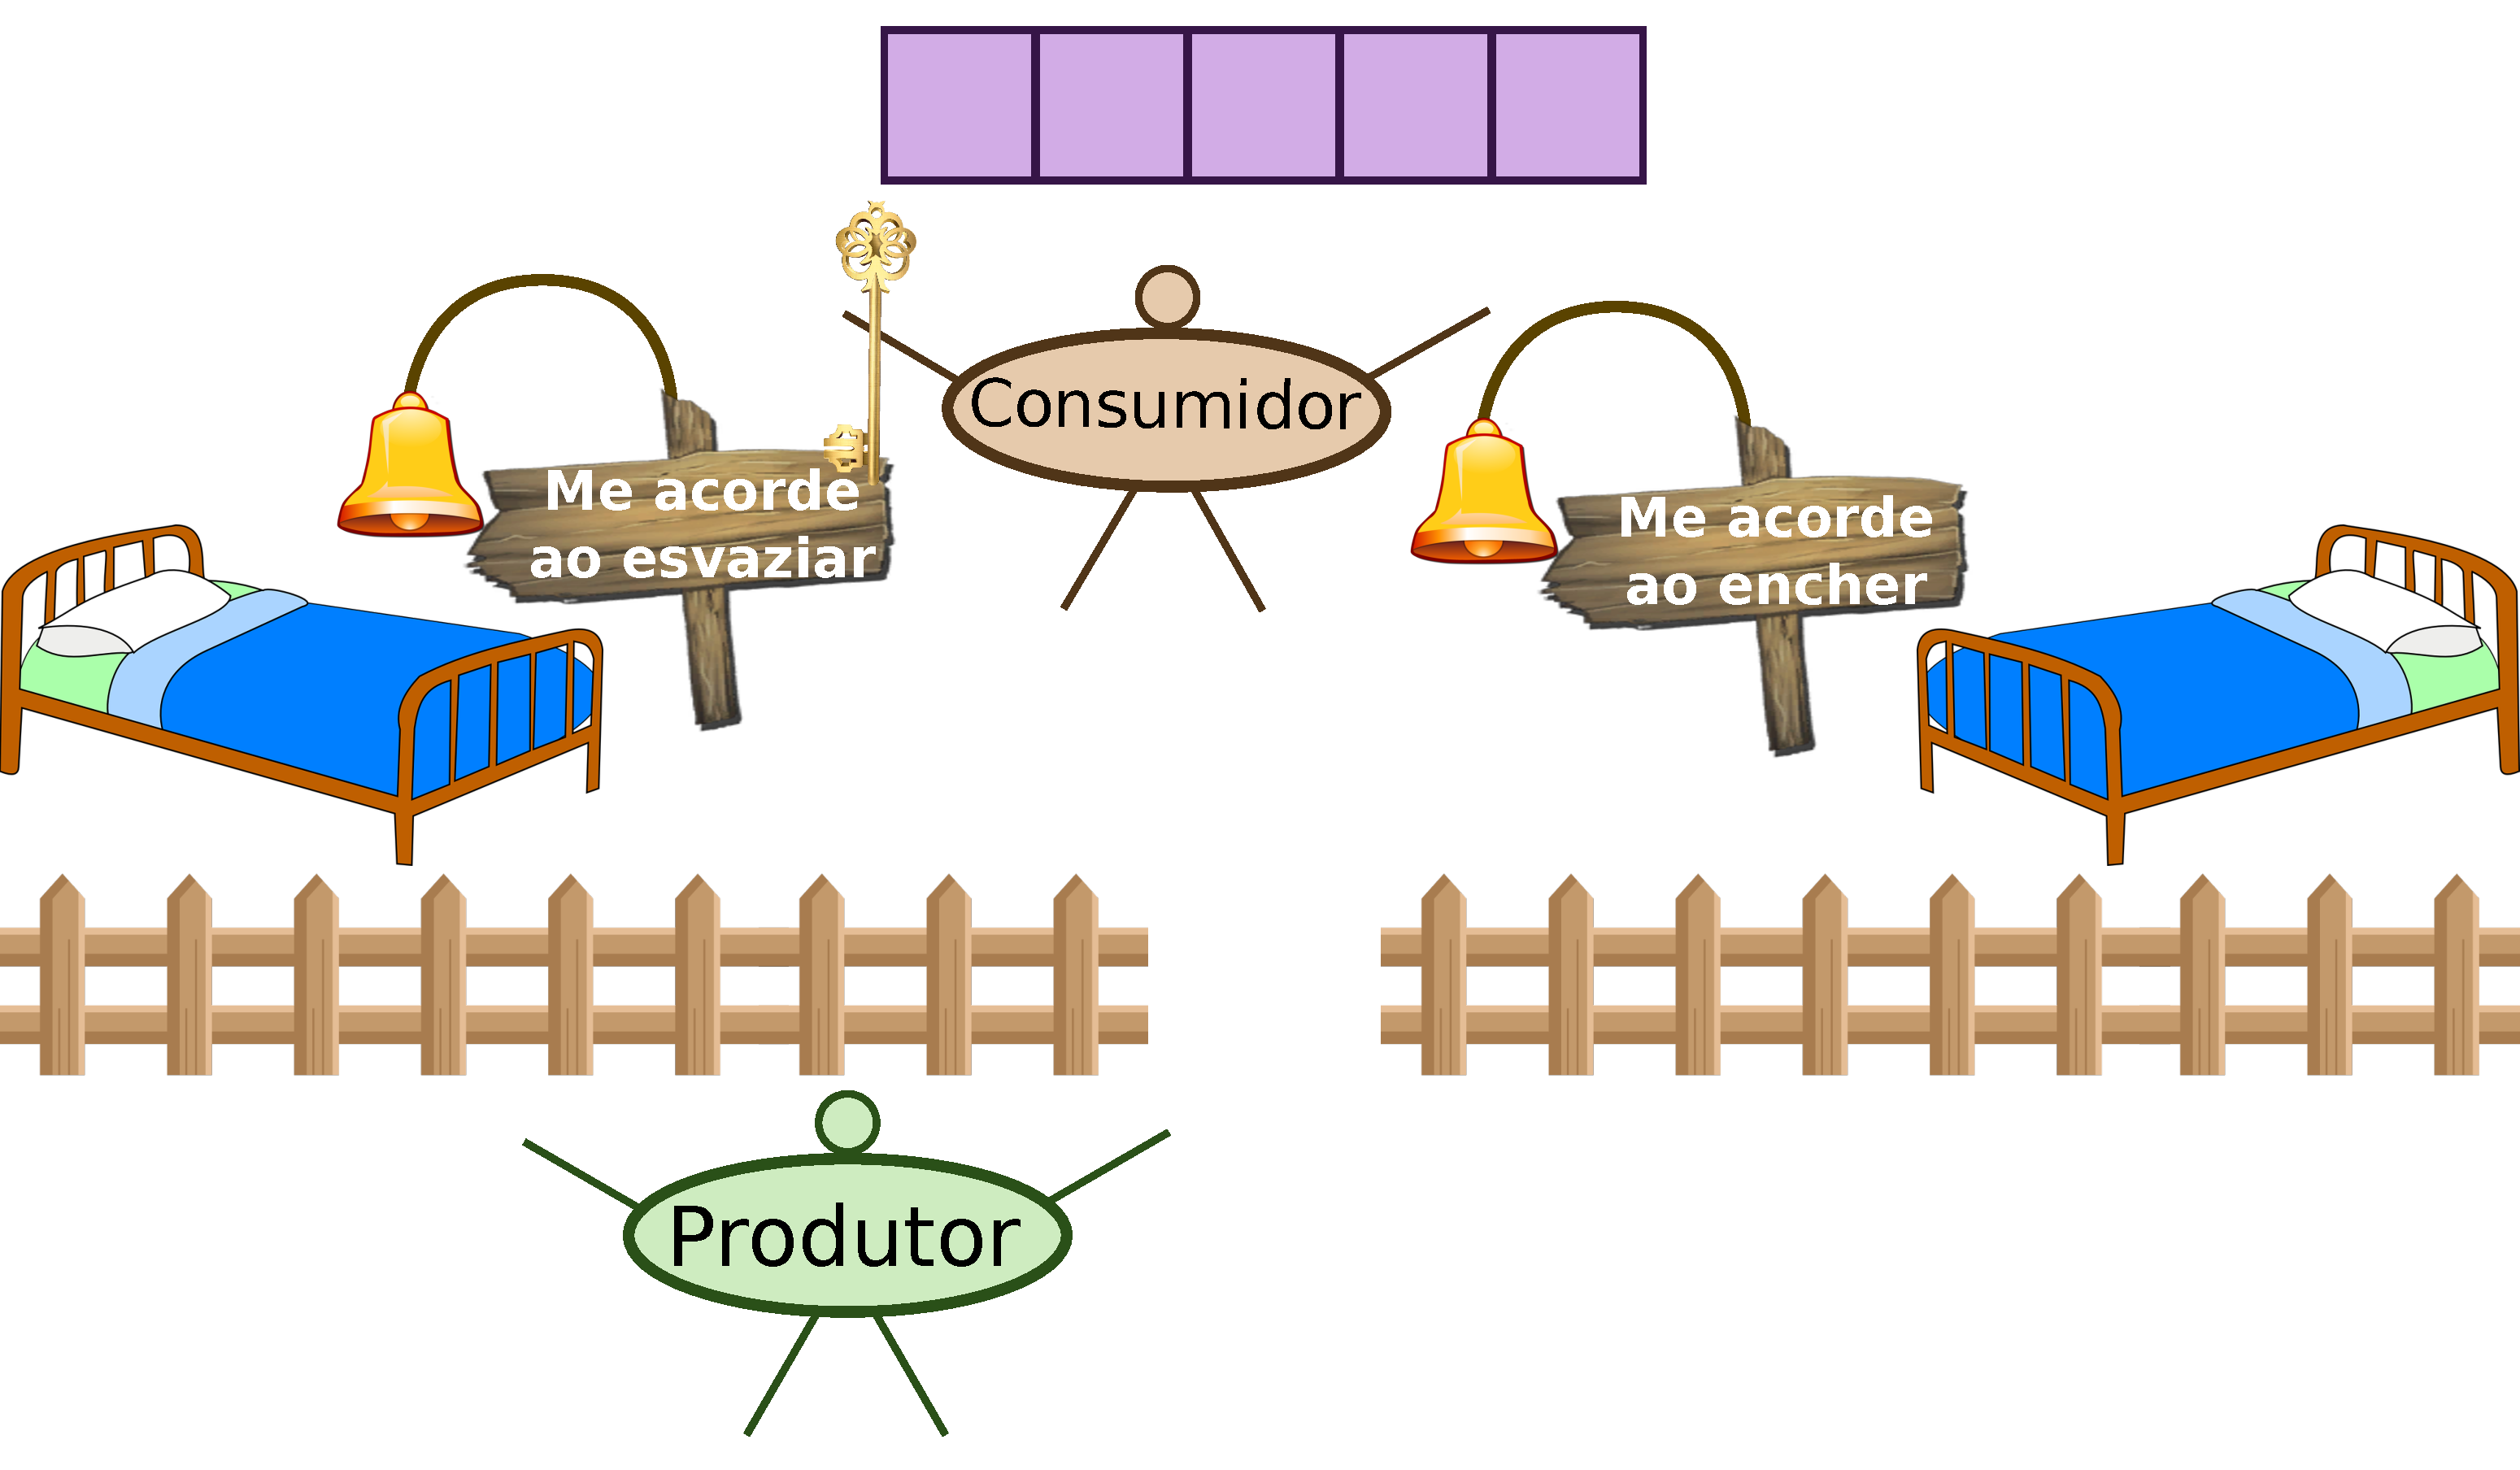
\includegraphics[width=0.9\paperwidth]{resources/cond2}}
		\only<3>{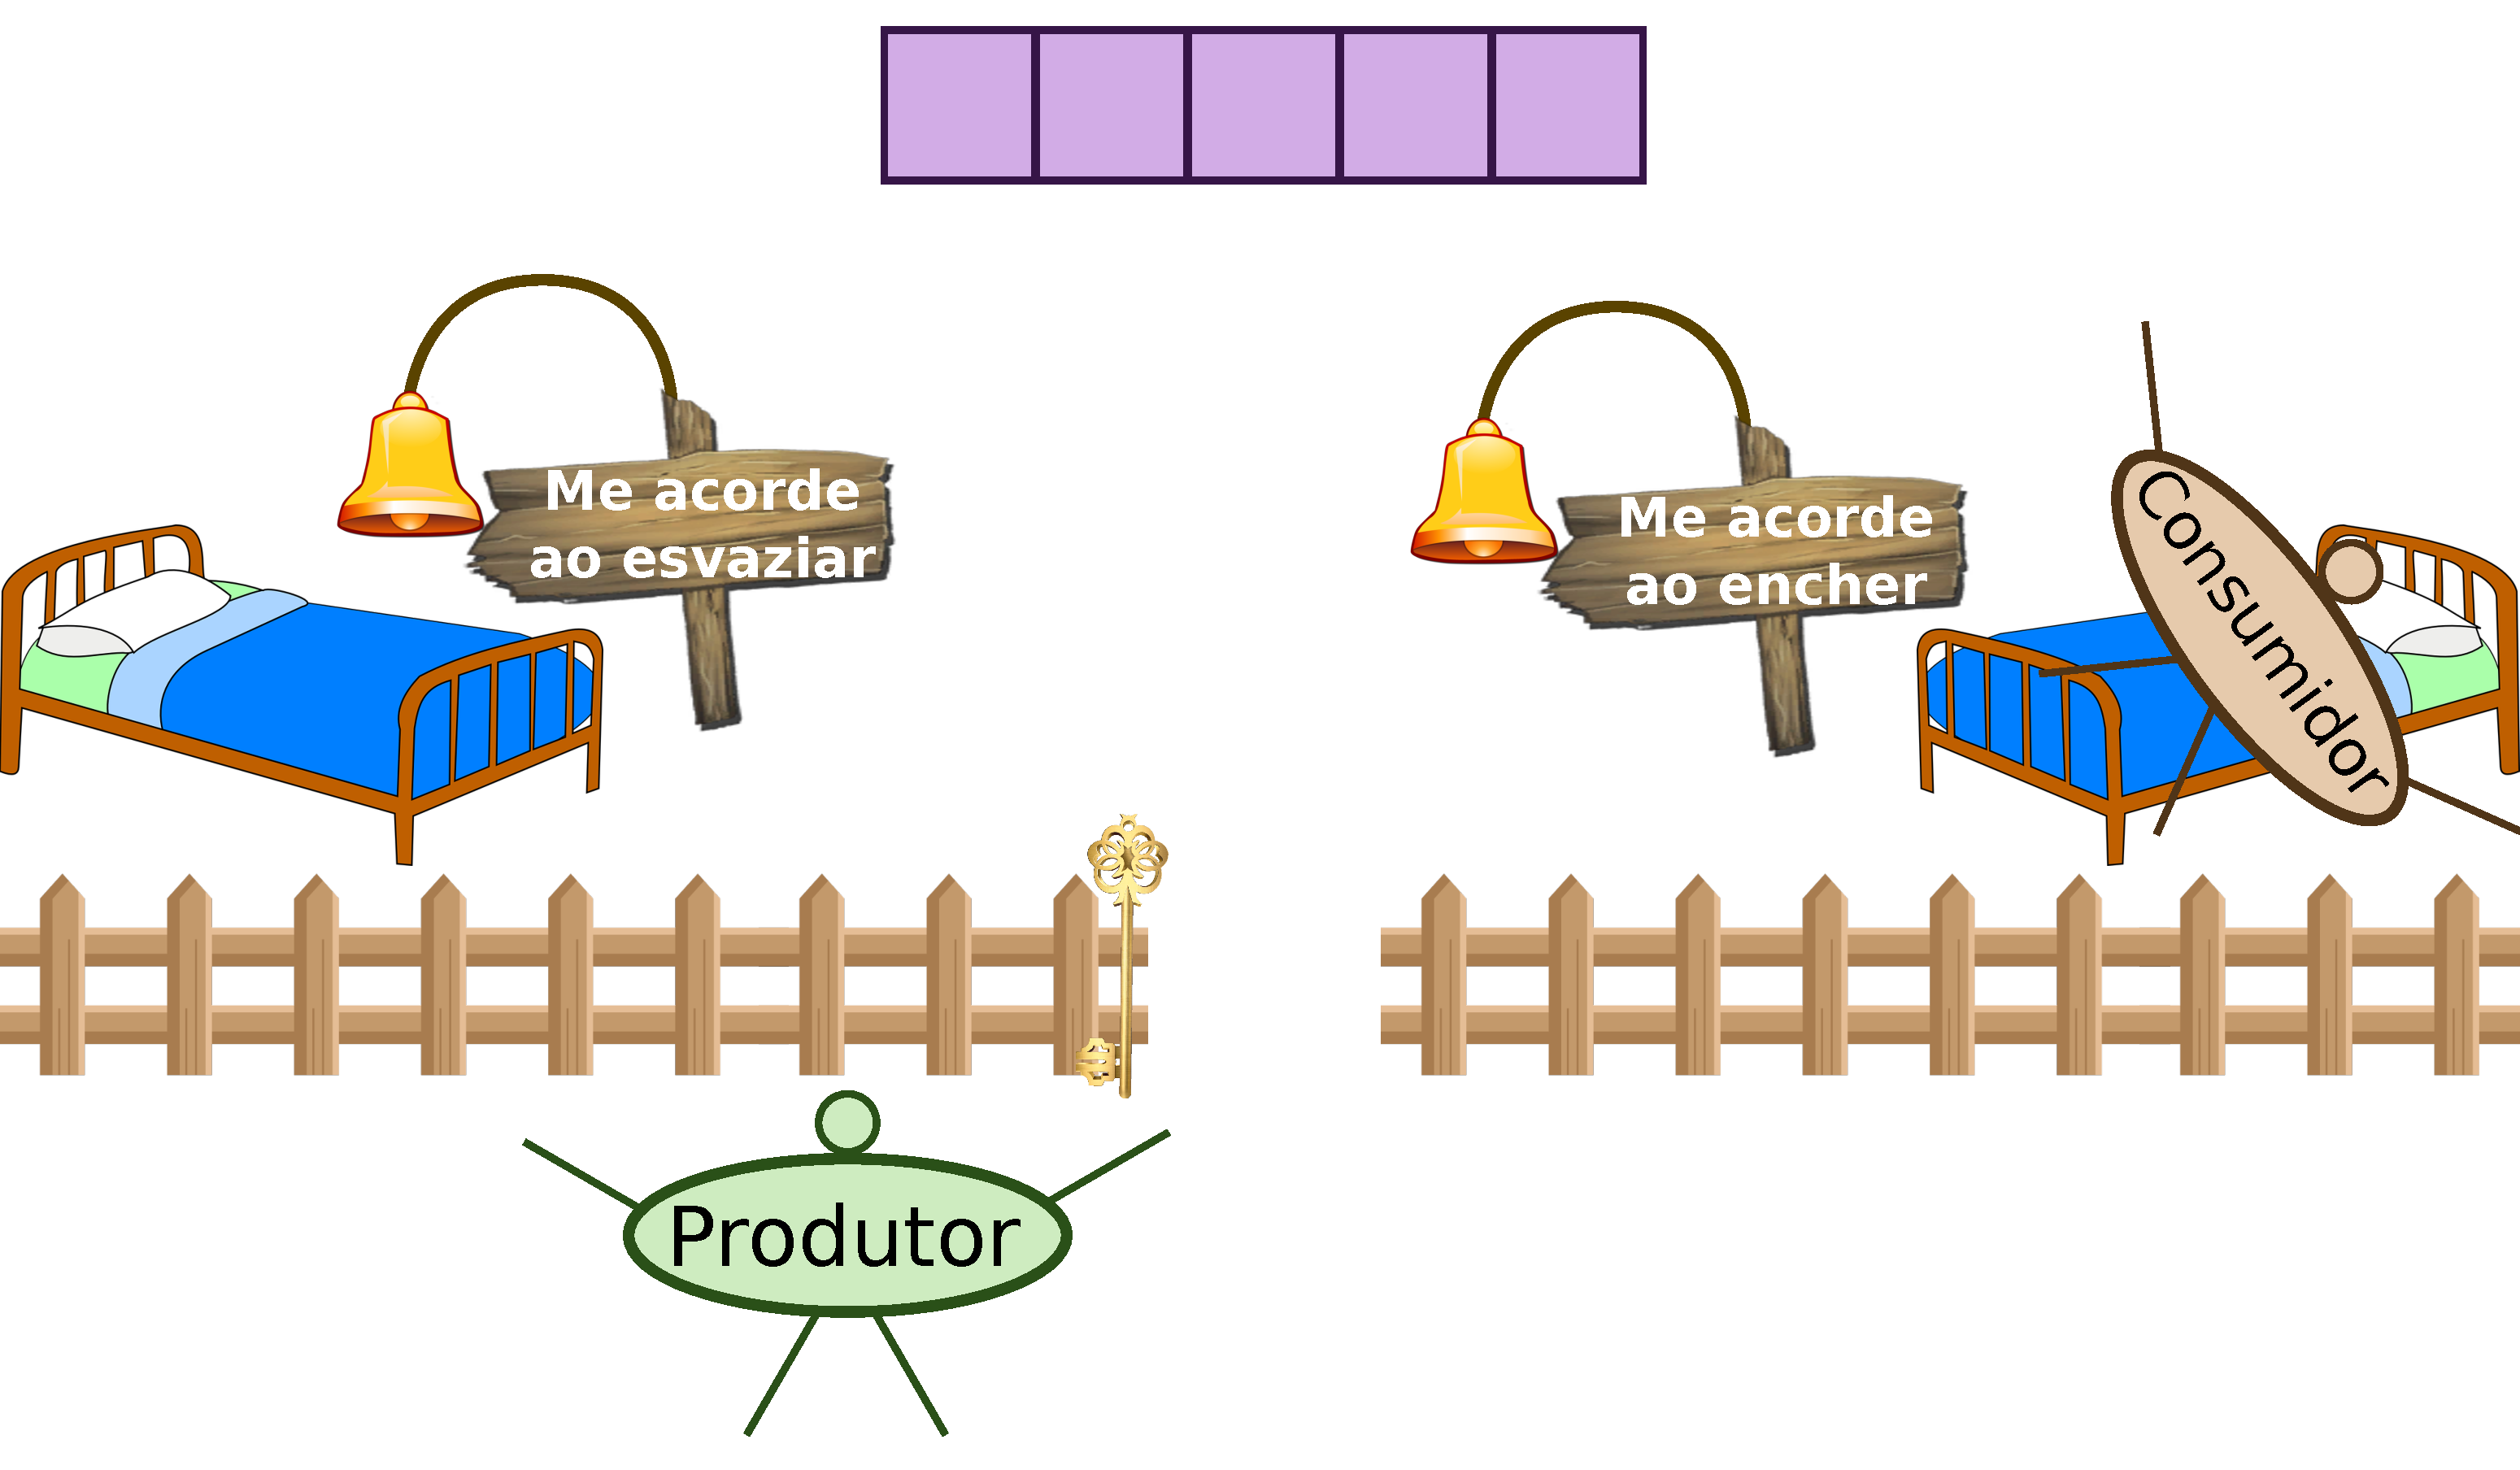
\includegraphics[width=0.9\paperwidth]{resources/cond3}}
		\only<4>{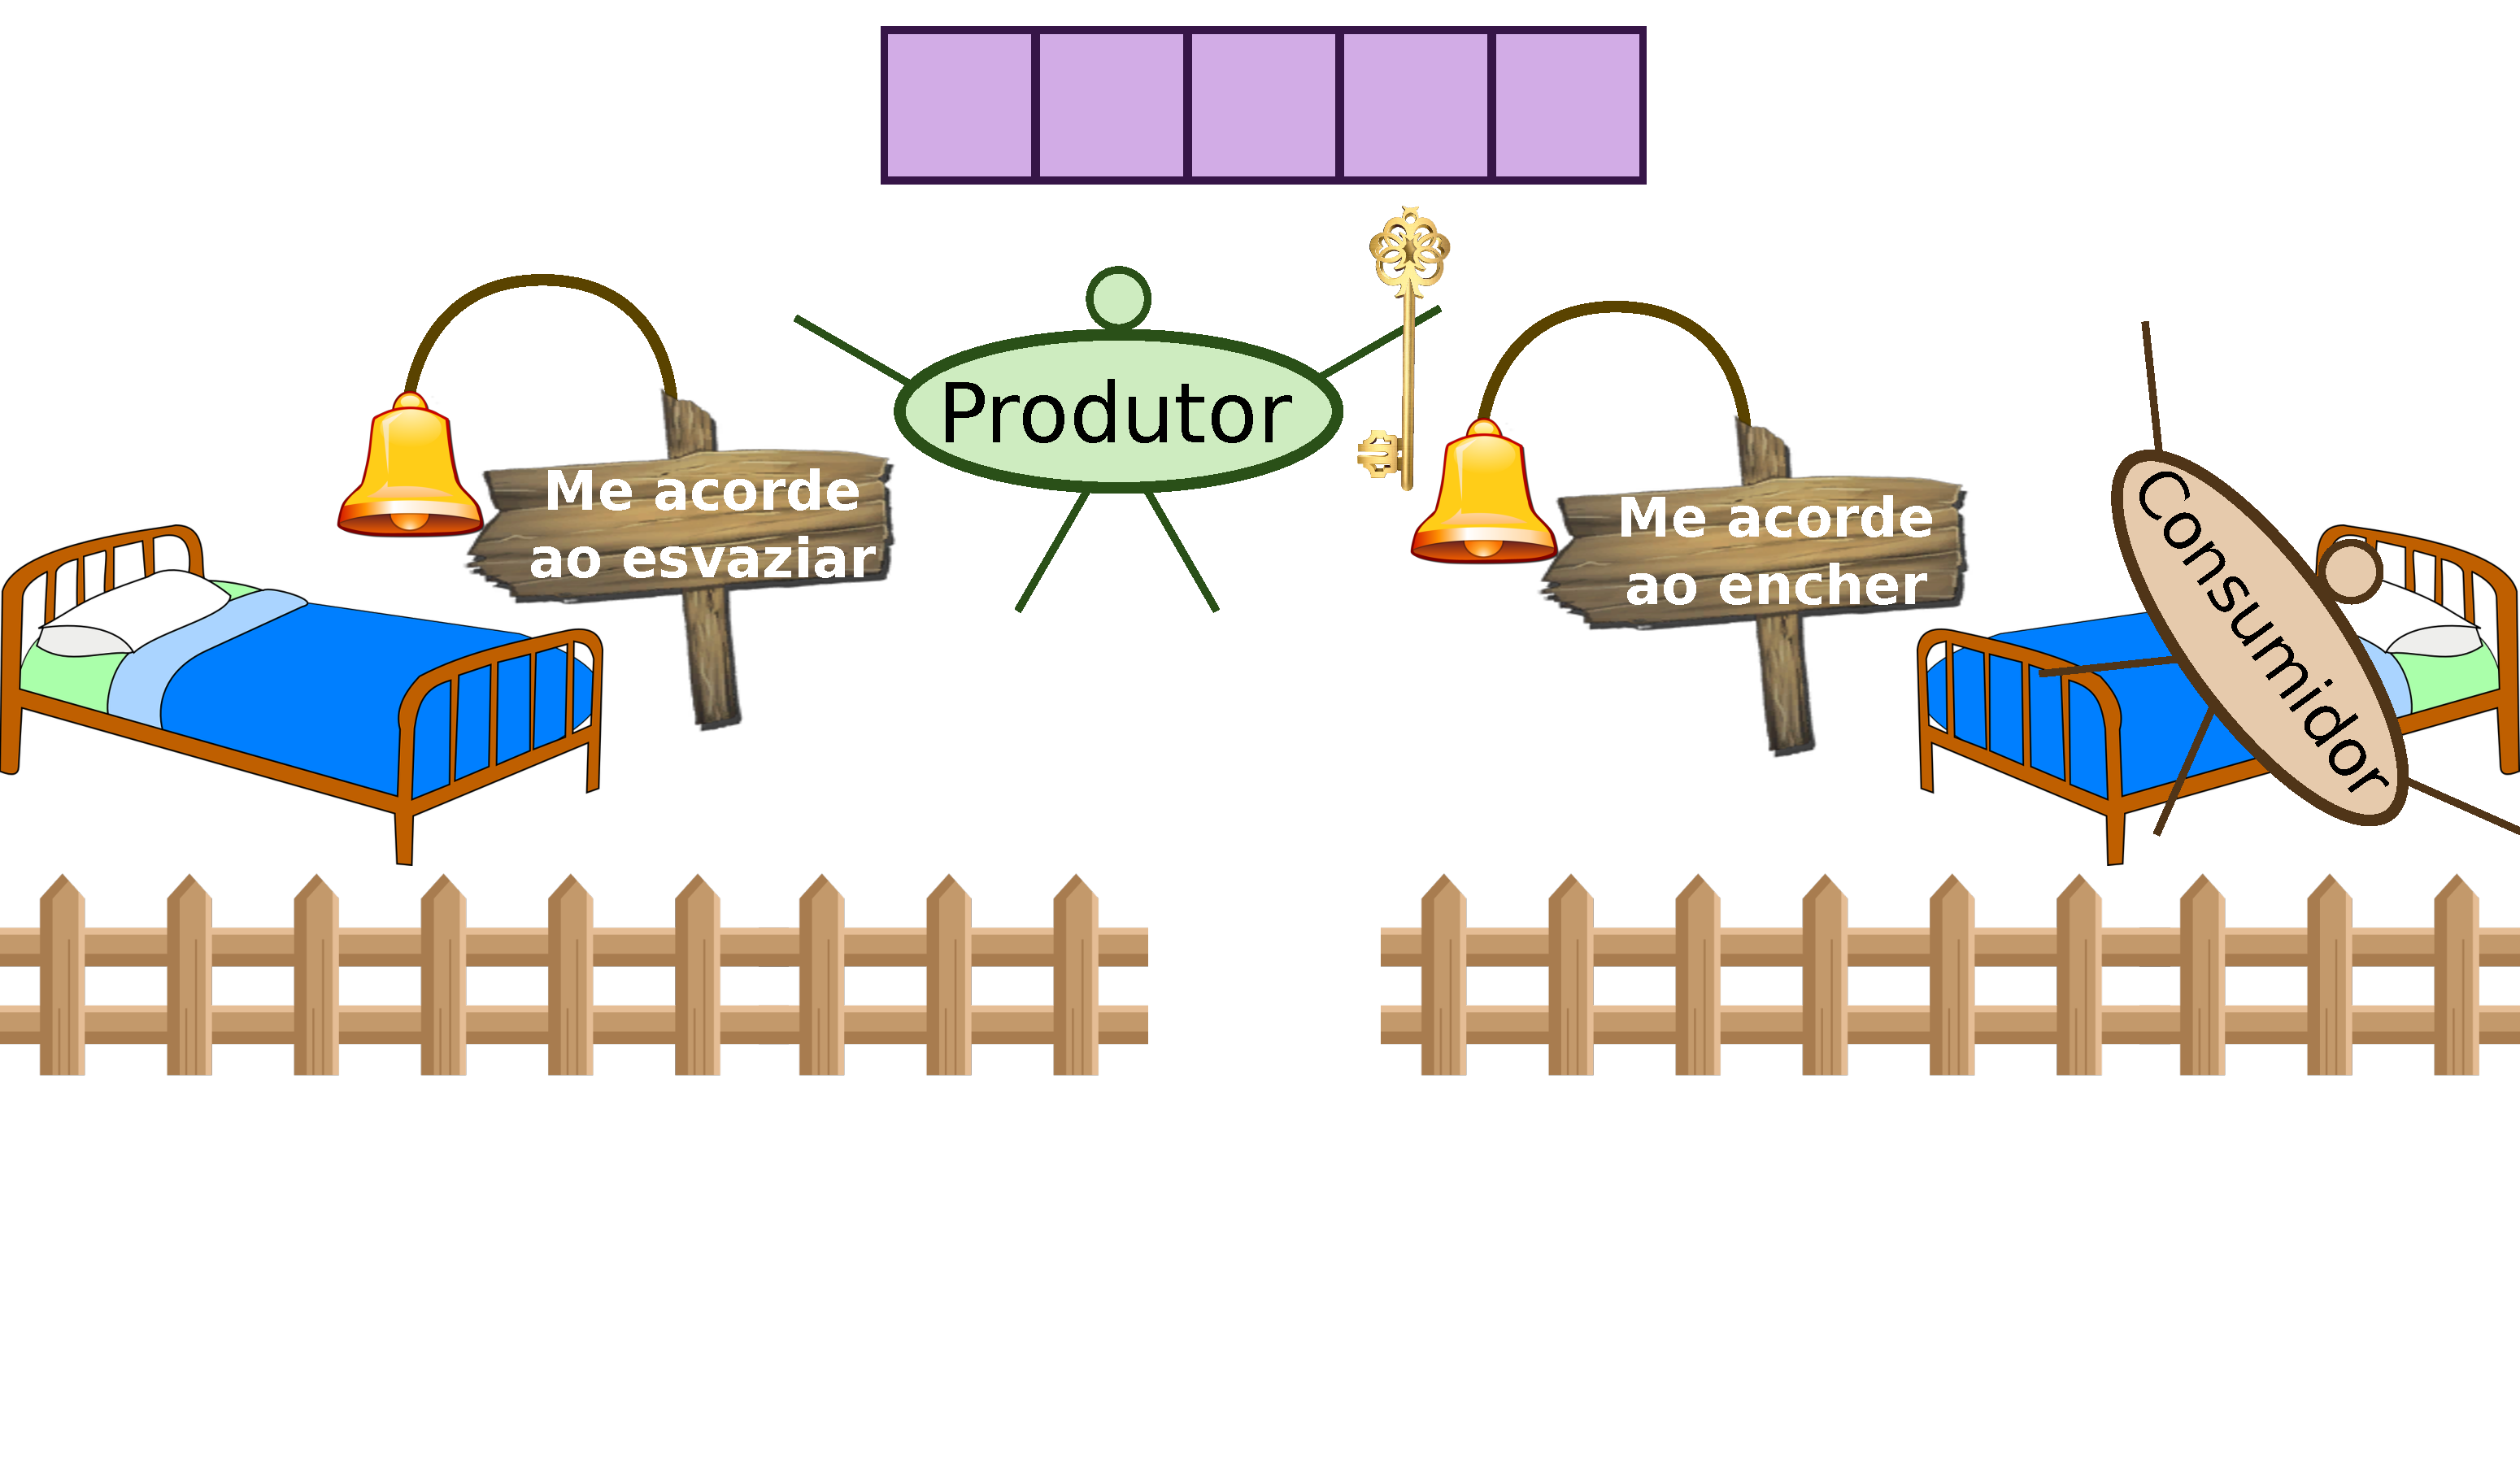
\includegraphics[width=0.9\paperwidth]{resources/cond4}}
		\only<5>{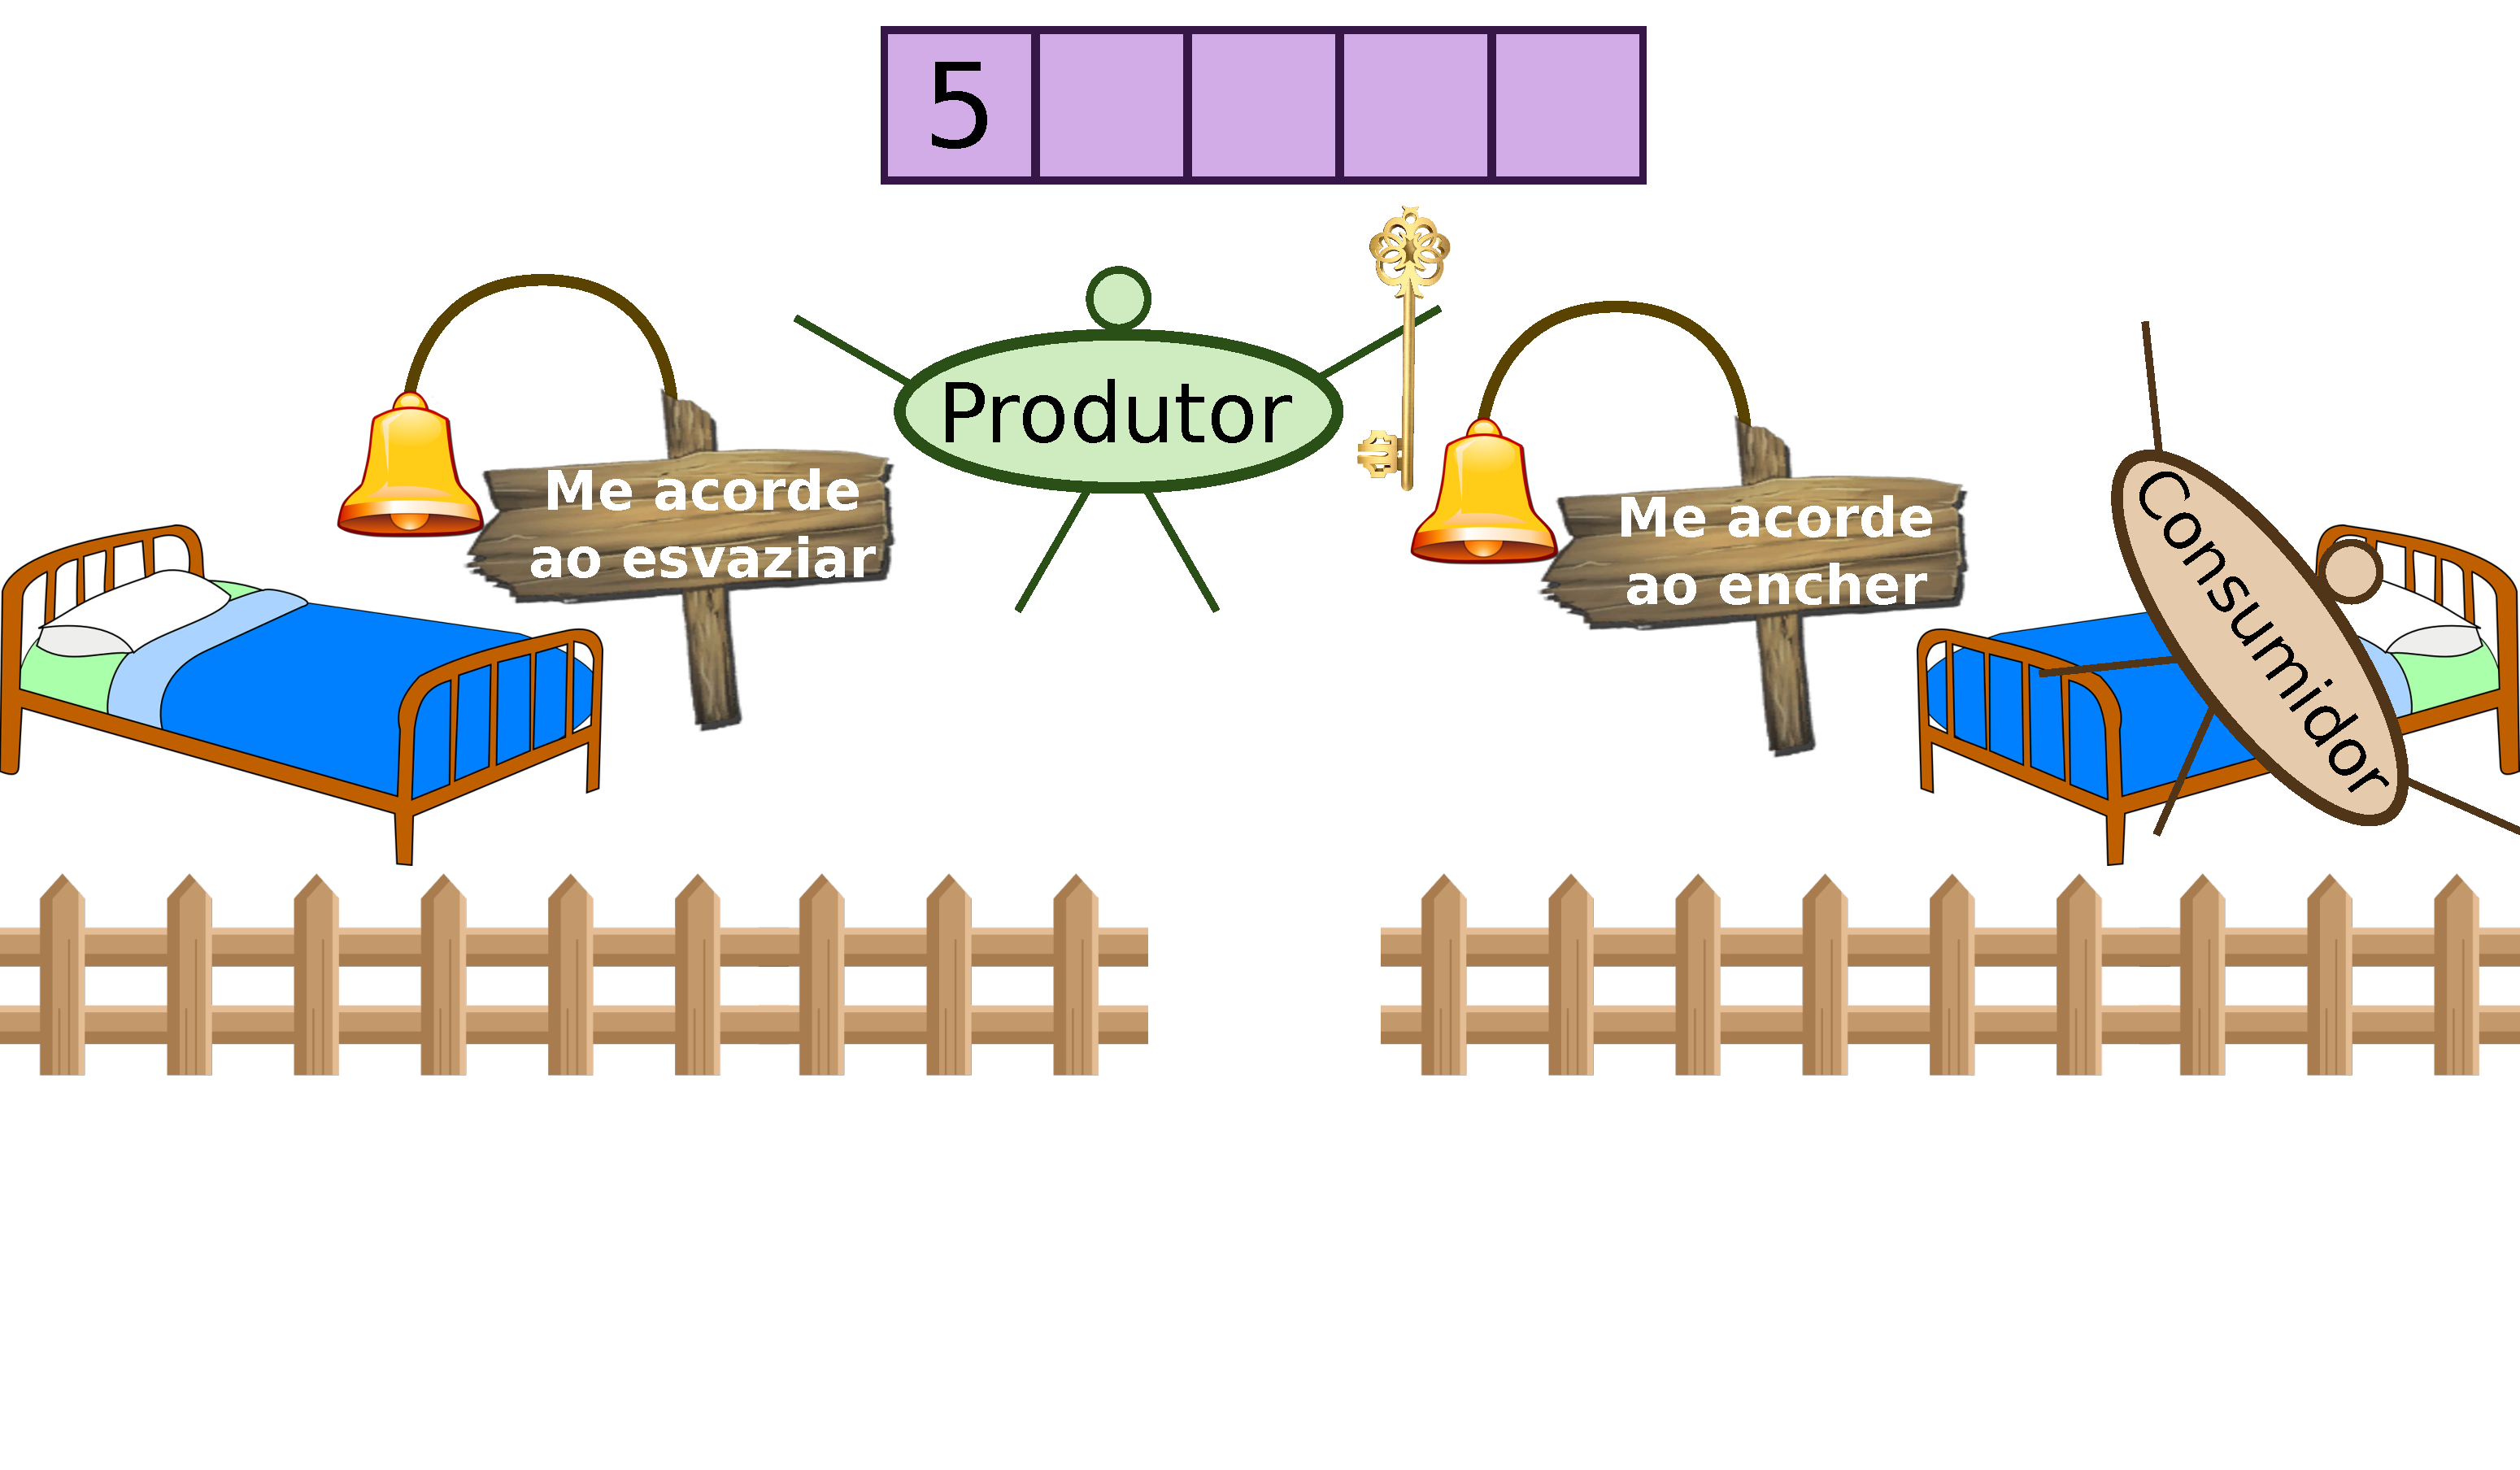
\includegraphics[width=0.9\paperwidth]{resources/cond5}}
		\only<6>{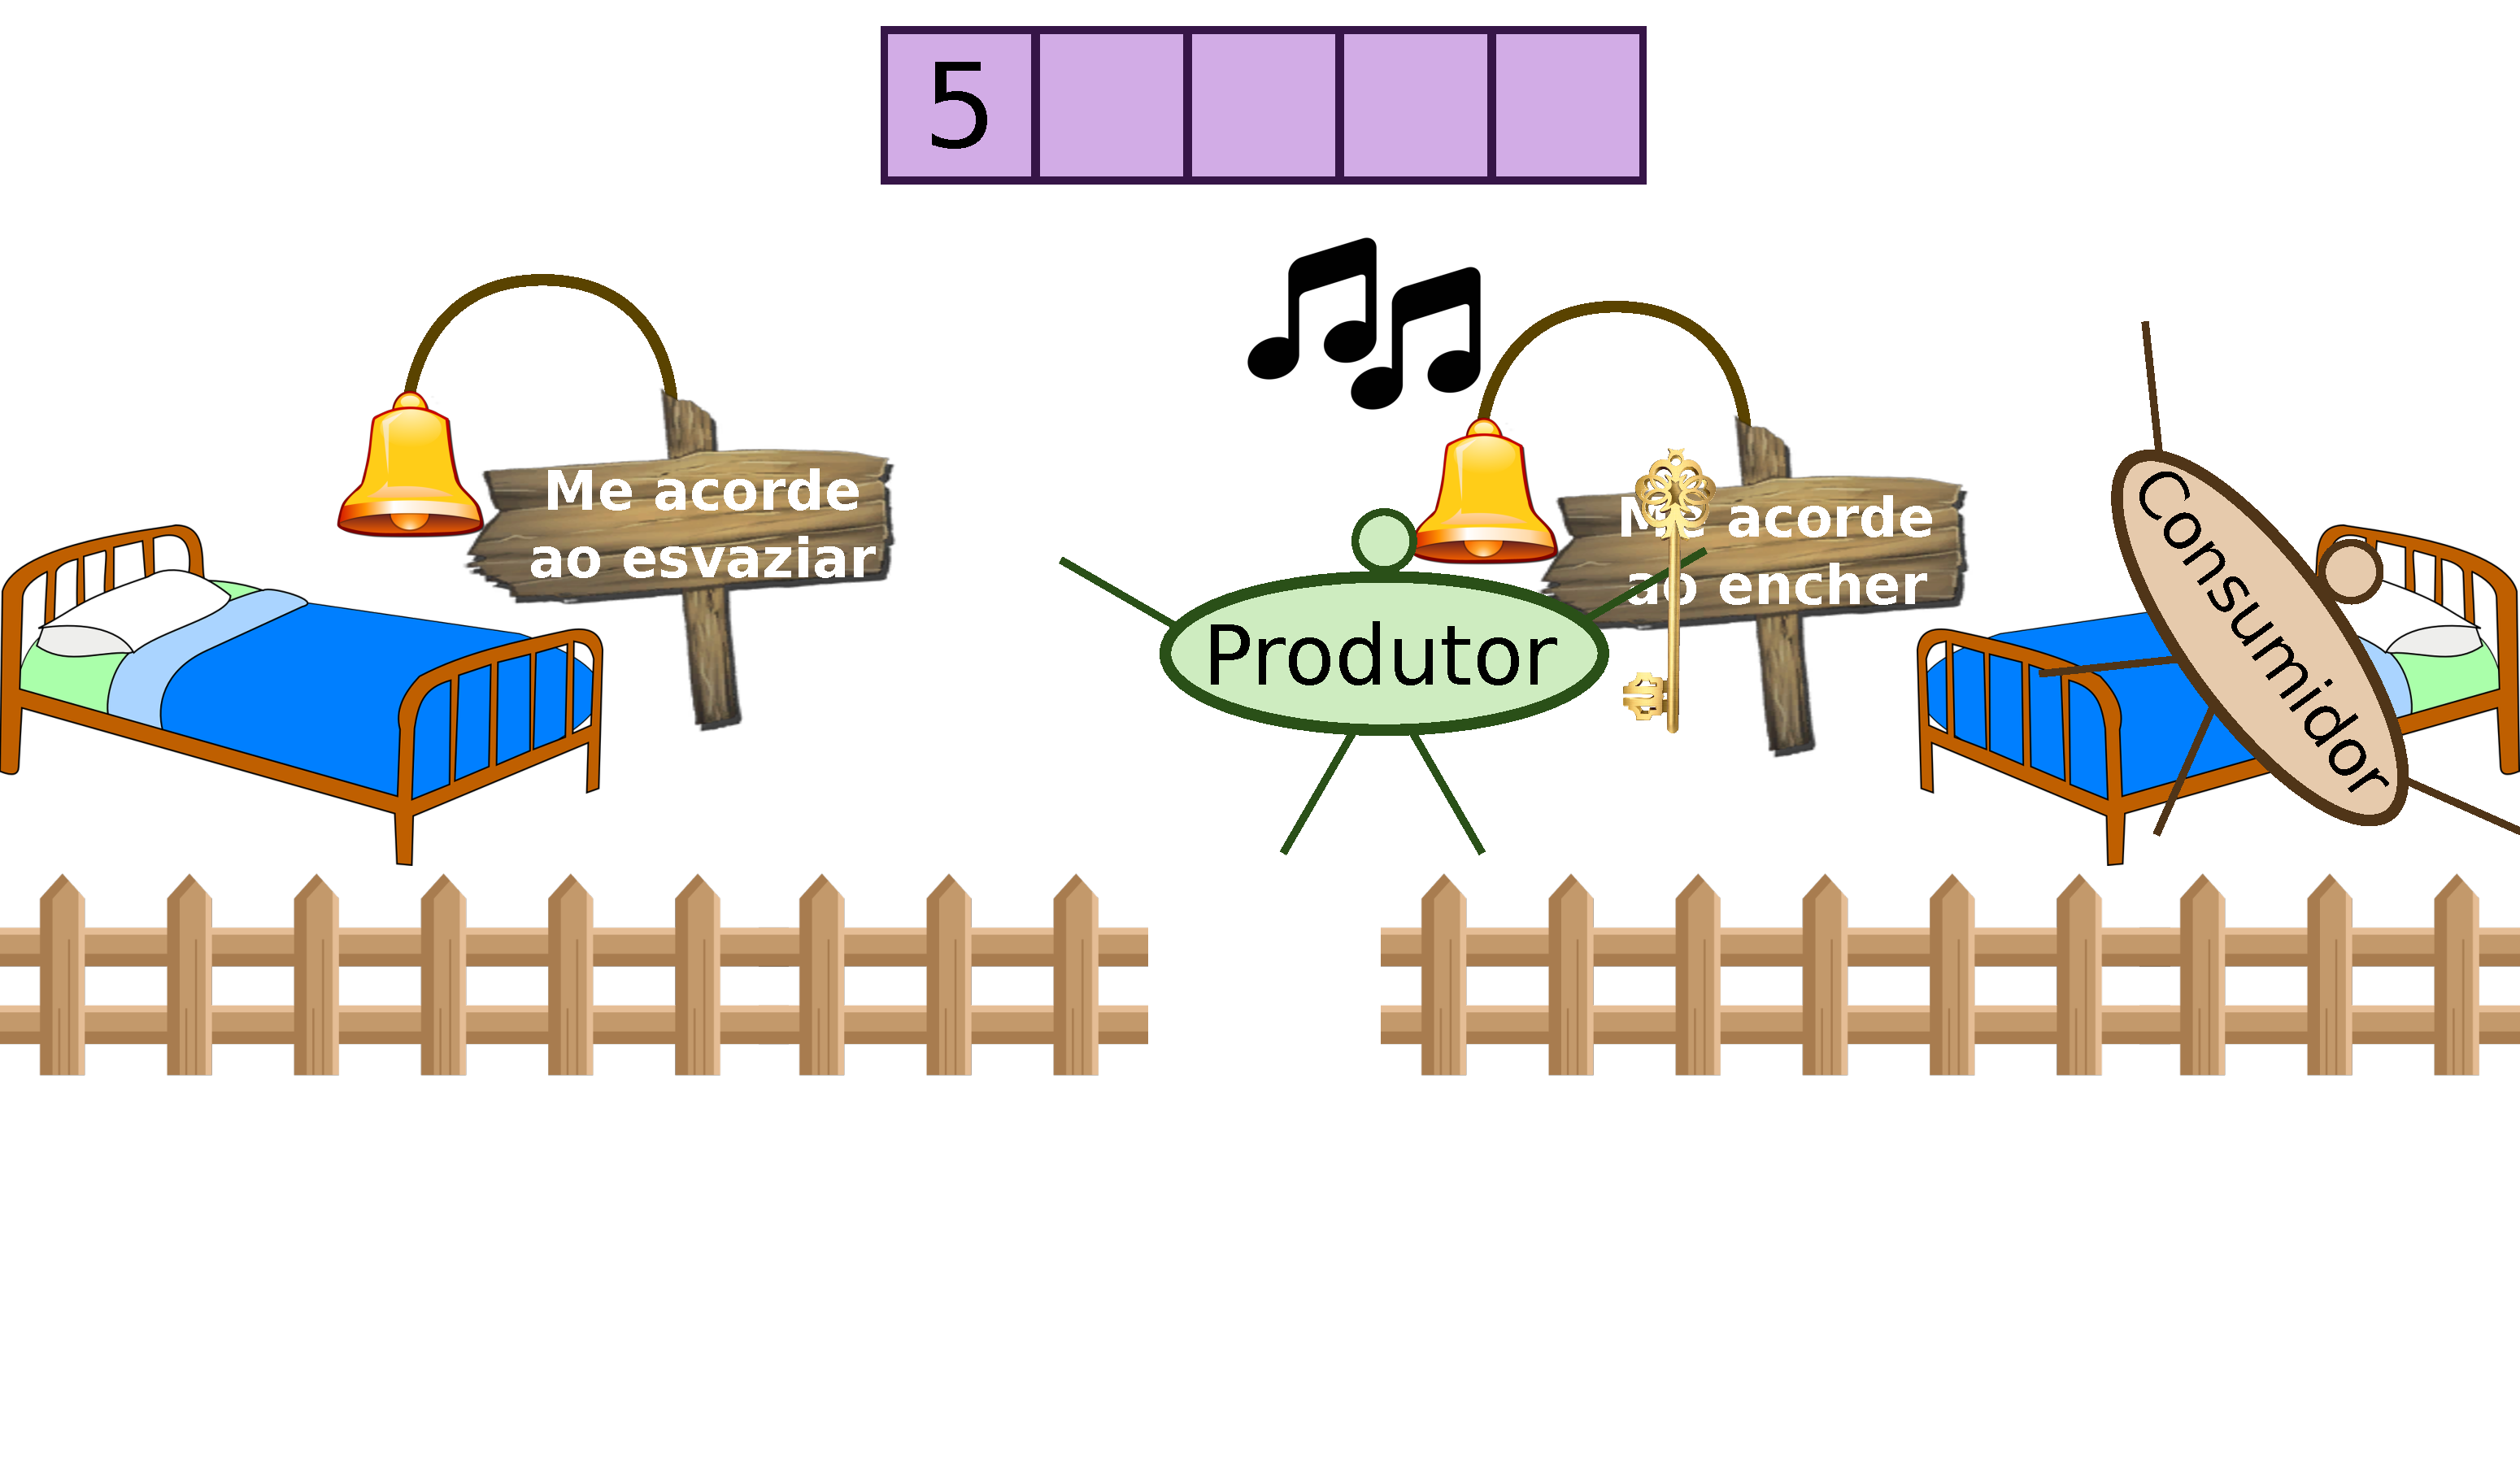
\includegraphics[width=0.9\paperwidth]{resources/cond6}}
		\only<7>{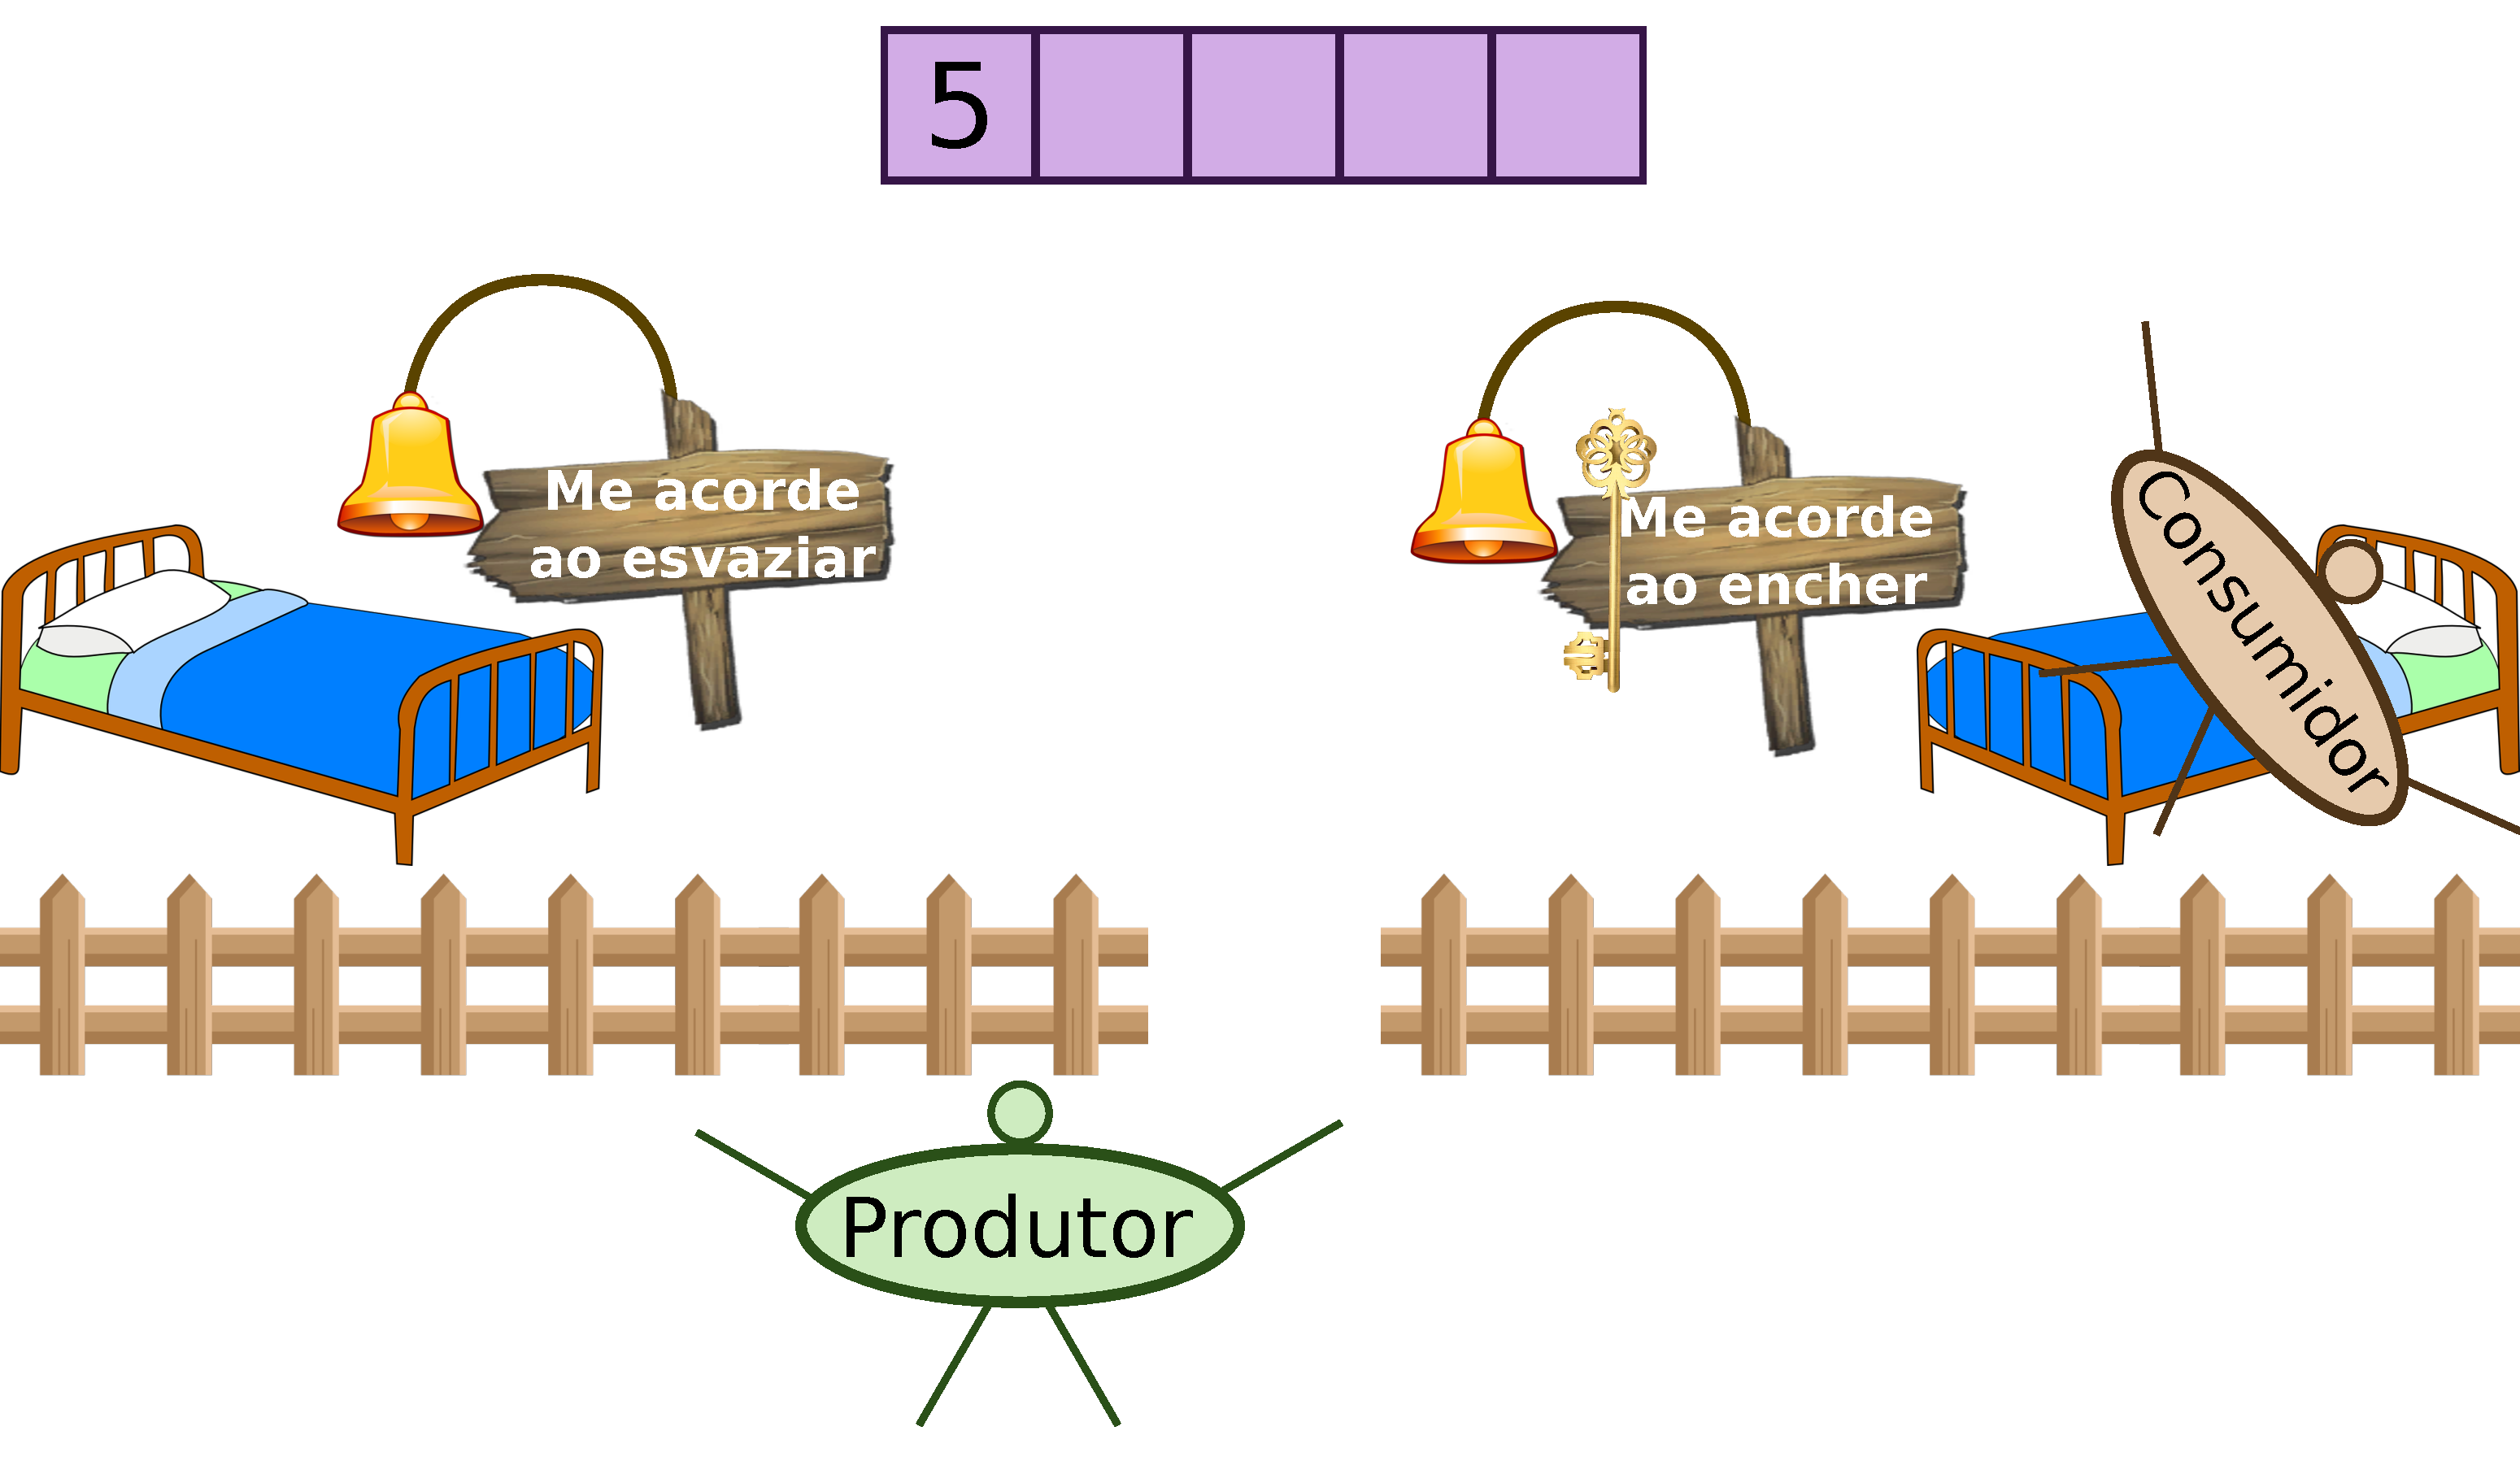
\includegraphics[width=0.9\paperwidth]{resources/cond7}}
		\only<8>{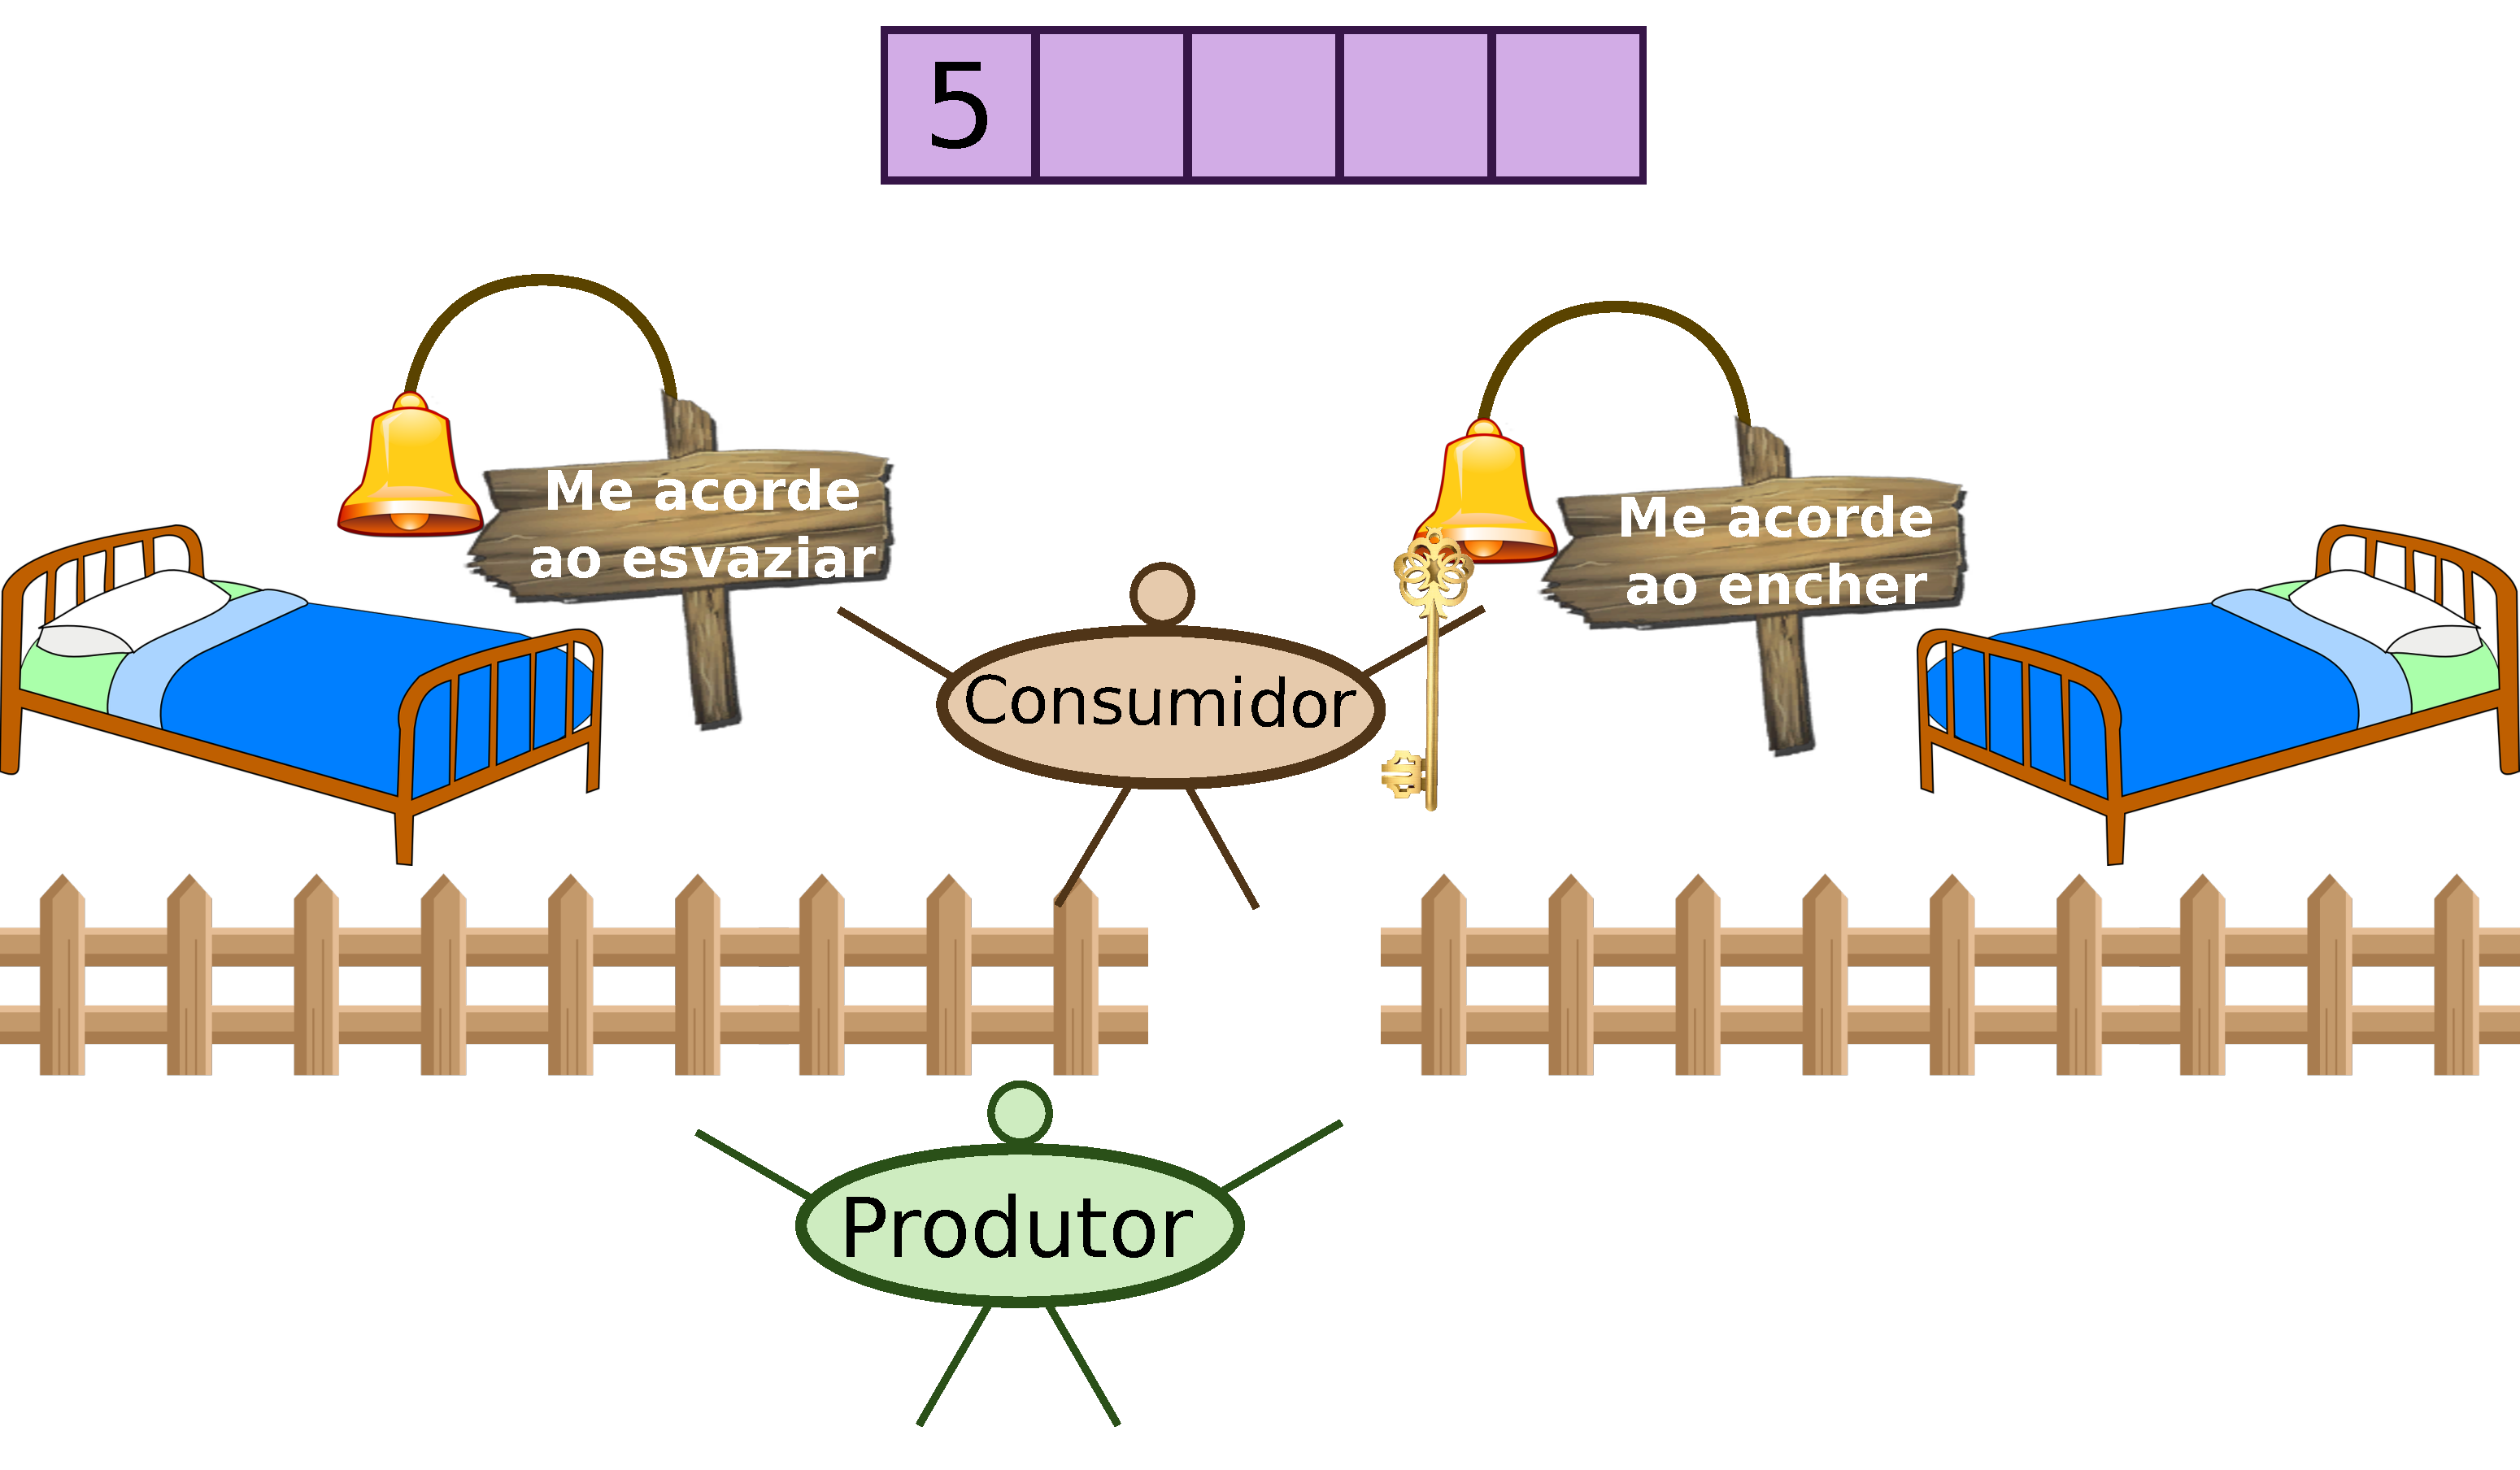
\includegraphics[width=0.9\paperwidth]{resources/cond8}}
		\only<9>{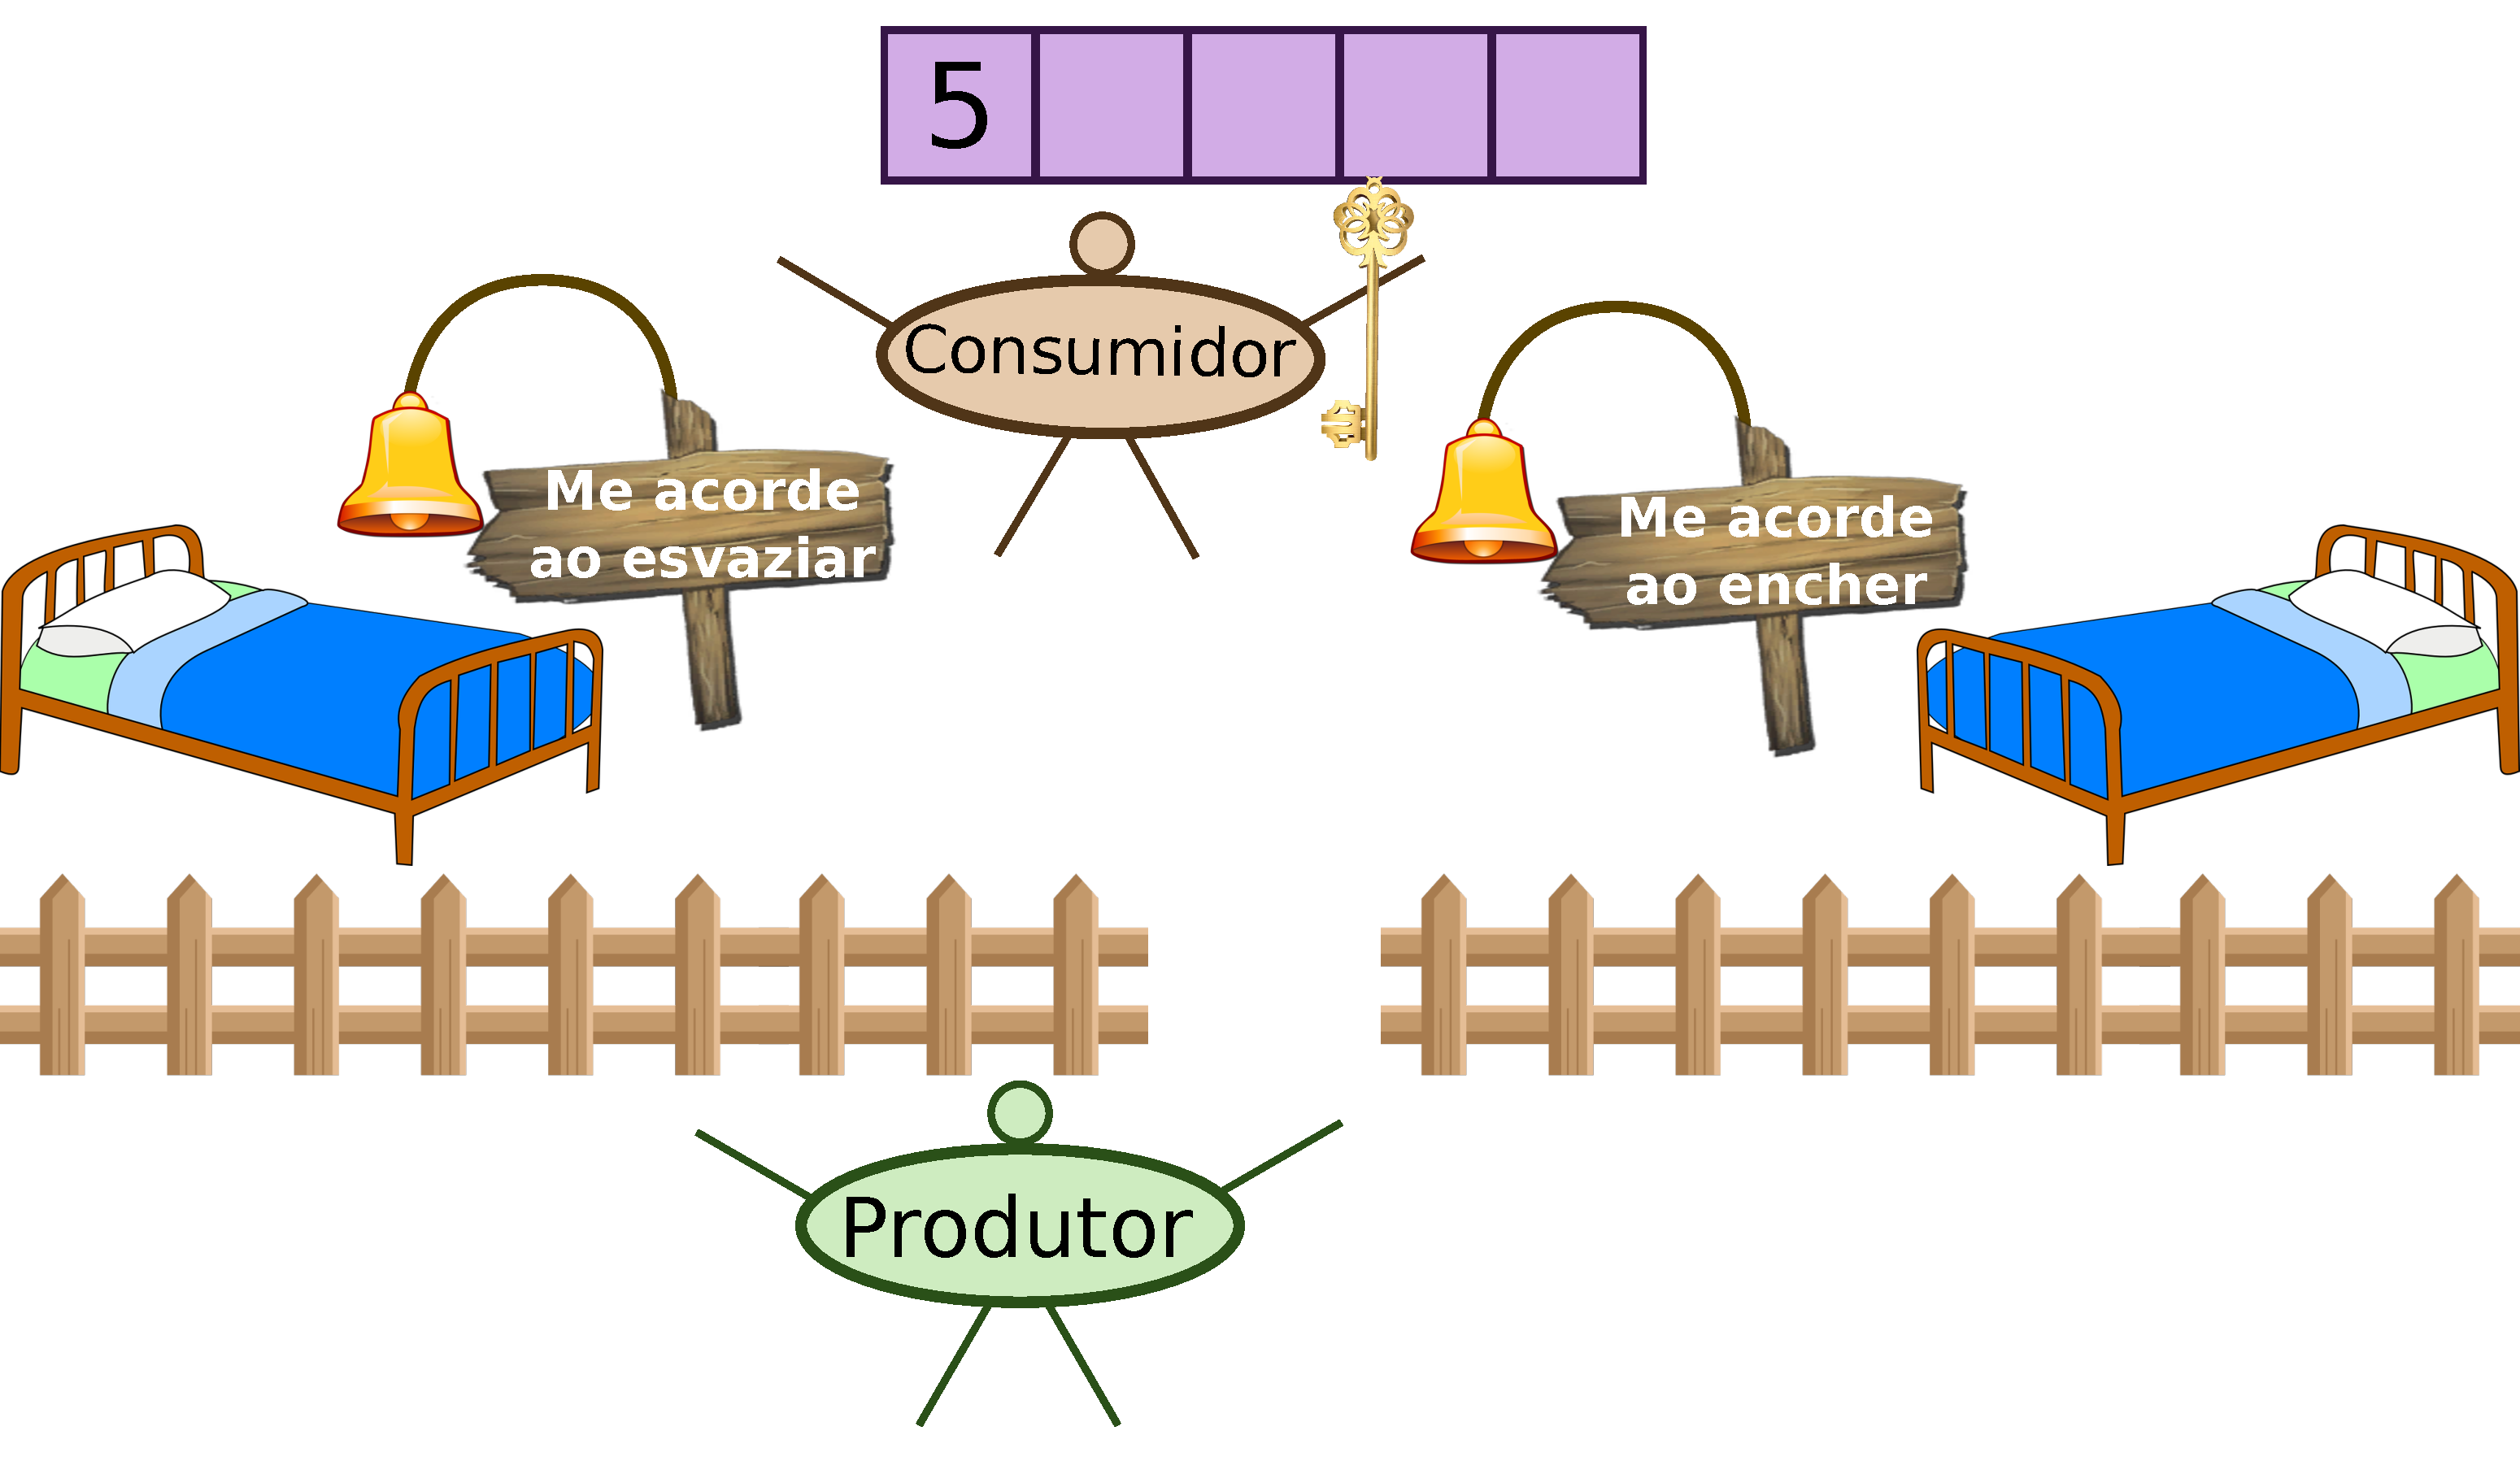
\includegraphics[width=0.9\paperwidth]{resources/cond9}}
		\only<10>{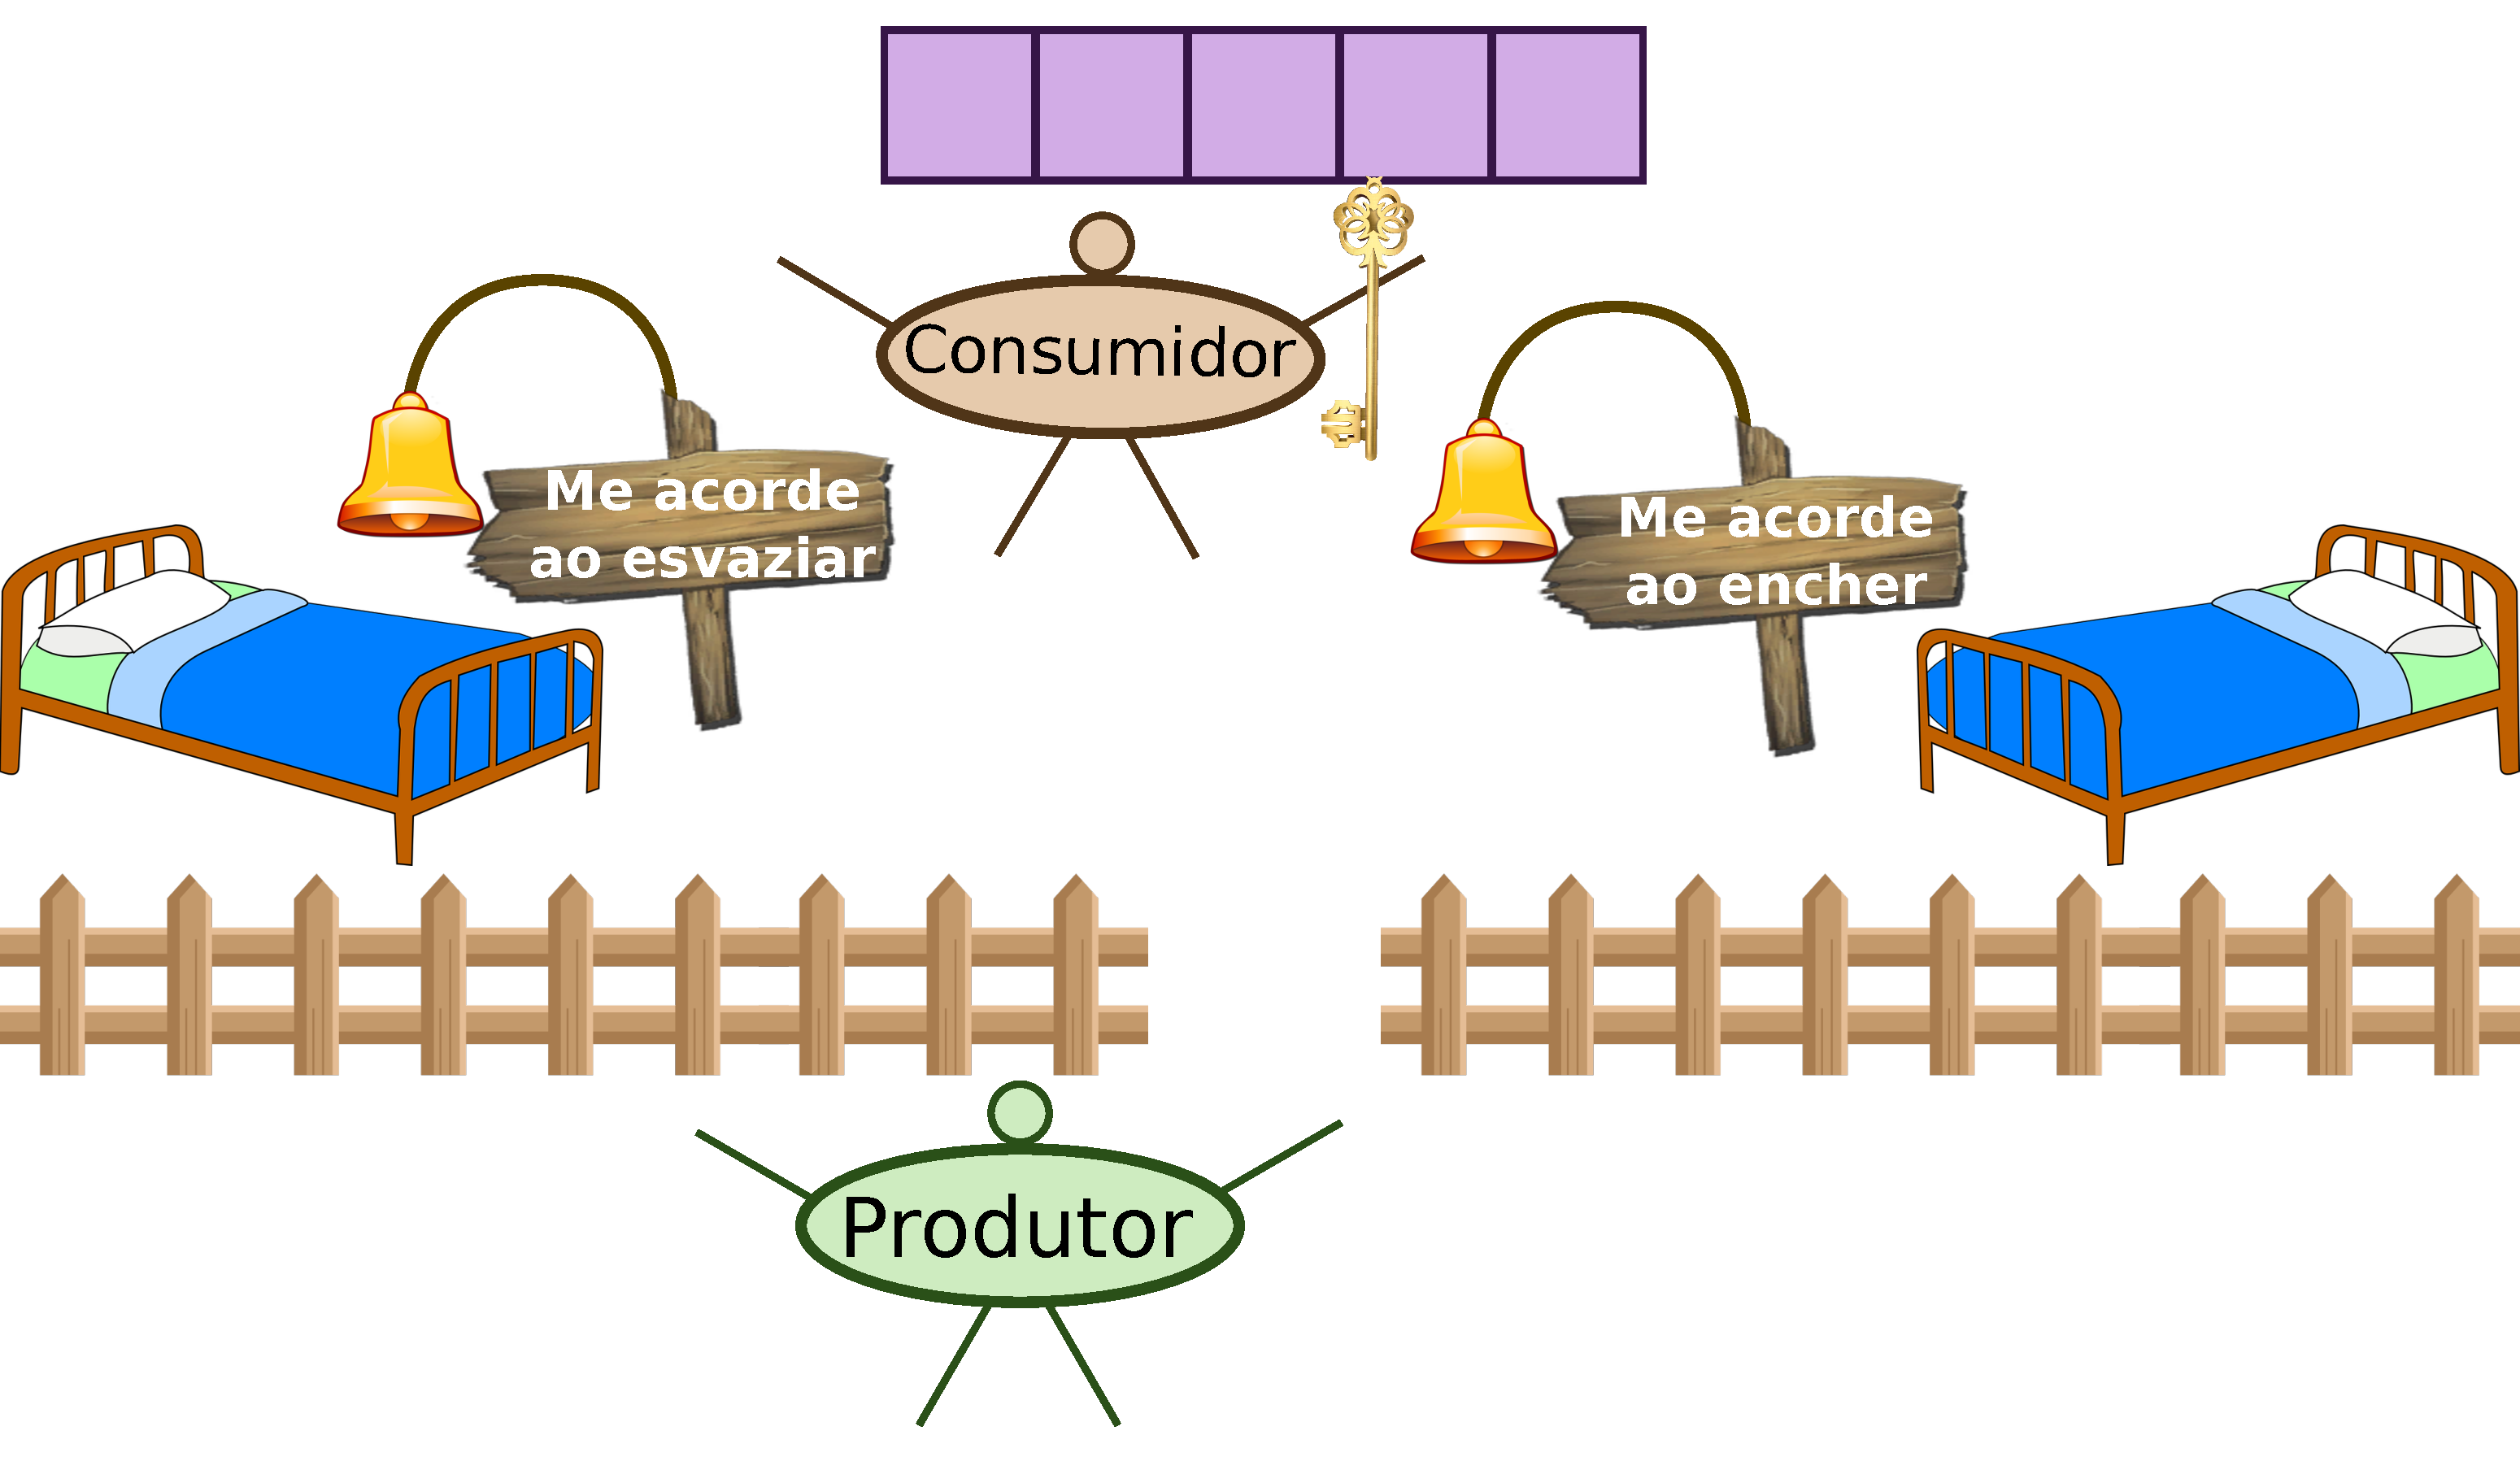
\includegraphics[width=0.9\paperwidth]{resources/cond10}}
		\only<11>{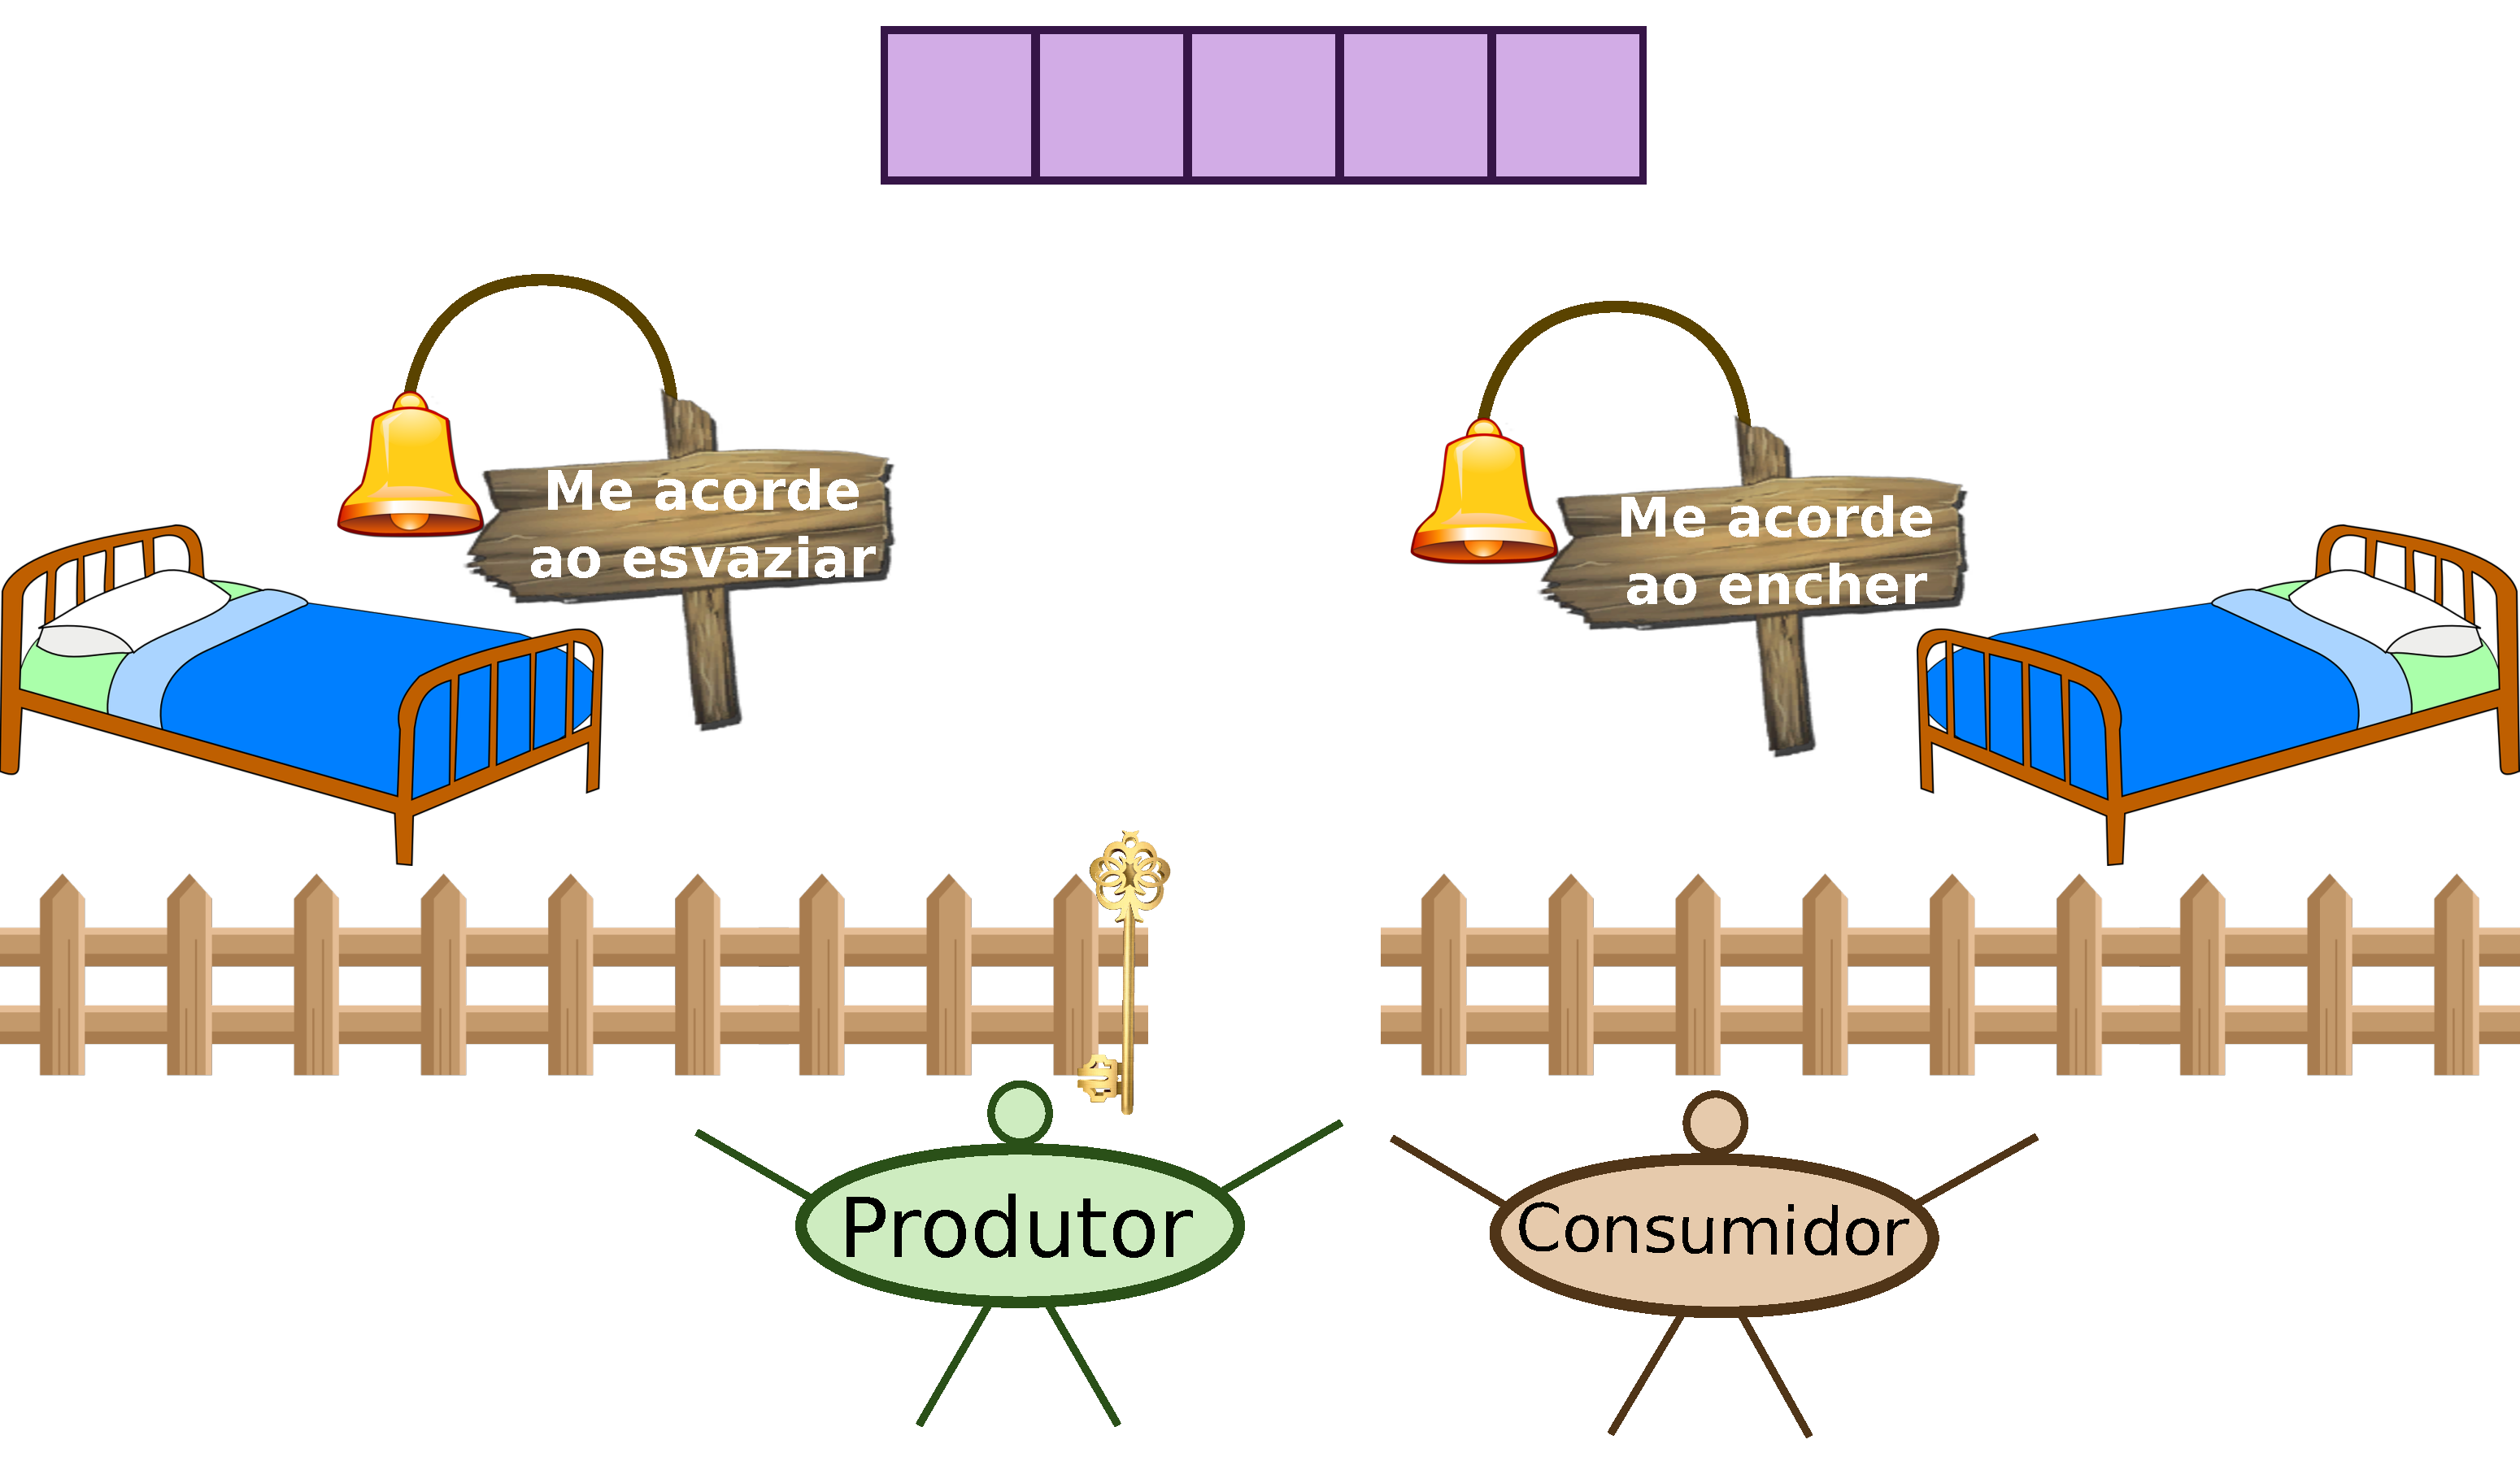
\includegraphics[width=0.9\paperwidth]{resources/cond11}}
	\end{figure}
\end{frame}
\begin{frame}{Condições de corrida}
	\framesubtitle{Variáveis de condição}
	\only<1>{\inputminted[fontsize=\footnotesize,lastline=6]{c}{resources/cond.c}}
	\only<2>{\inputminted[fontsize=\footnotesize,firstline=8,lastline=18]{c}{resources/cond.c}}
	\only<3>{\inputminted[fontsize=\footnotesize,firstline=20,lastline=30]{c}{resources/cond.c}}
	\only<4>{\inputminted[fontsize=\footnotesize,firstline=32,lastline=44]{c}{resources/cond.c}}
\end{frame}
\begin{frame}{Condições de corrida}
	\framesubtitle{Monitores}
	\begin{itemize}
		\item Semáforos e mutexes são complicados de usar
		\item \textbf{Monitores} são primitivas de sincronização de mais alto nível
		\item \textbf{Ideia:} mover os métodos e estruturas para dentro de um monitor
		\item Processos podem chamar métodos do monitor, mas não podem acessar as estruturas internas
		\item \textbf{Somente um processo pode estar dentro do monitor}
		\item O compilador cuida de garantir a exclusão mútua
		\item Também utilizamos variáveis de condição (\texttt{wait} e \texttt{signal}) para que um processo possa esperar por alguma condição
	\end{itemize}
\end{frame}
\begin{frame}{Condições de corrida}
	\framesubtitle{Passagem de mensagens}
	\begin{itemize}
		\item Todos os métodos que utilizamos até agora só funcionam em uma mesma máquina
		\item E se quiséssemos sincronizar processos em máquinas diferentes?
		\item \textbf{Passagem de mensagens} é feita com o uso de duas primitivas: \textbf{send} e \textbf{receive}
	\end{itemize}
\end{frame}
\begin{frame}{Condições de corrida}
	\framesubtitle{Passagem de mensagens}
	\begin{itemize}
		\item Passagem de mensagens introduz uma série de novos problemas:
		\begin{itemize}
			\item E se uma mensagem é perdida pela rede?\pause
			\begin{itemize}
				\item O destinatário avisa quando receber a mensagem (acknowledgement)
				\item Se o remetente não recebe o acknowledgement a tempo, reenvia a mensagem
			\end{itemize}\pause
			\item E se o acknowledgement é perdido?\pause
			\begin{itemize}
				\item O remetente envia novamente a mensagem. O destinatário recebe duas cópias da mensagem
				\item Numeramos cada mensagem
			\end{itemize}
		\end{itemize}
		\item Outros desafios são tratados na disciplina de \textbf{Redes}
	\end{itemize}
\end{frame}
\begin{frame}{Condições de corrida}
	\framesubtitle{Passagem de mensagens}
	\begin{columns}
		\begin{column}{0.5\textwidth}
			\inputminted[lastline=13,fontsize=\footnotesize]{c}{resources/messagepassing.c}
		\end{column}
		\begin{column}{0.5\textwidth}
			\inputminted[firstline=15,fontsize=\footnotesize]{c}{resources/messagepassing.c}
		\end{column}
	\end{columns}
\end{frame}
\begin{frame}{Condições de corrida}
	\framesubtitle{Barreiras}
	\begin{itemize}
		\item Utilizada quando diversos processos estão trabalhando em conjunto
		\item Ao encontrar uma barreira, o processo bloqueia até que \textbf{todos} os outros processos também cheguem até a barreira
		\item \textbf{Exemplo:} um cálculo iterativo com matrizes
	\end{itemize}
\end{frame}
\begin{frame}{Condições de corrida}
	\framesubtitle{Barreiras}
	\begin{figure}
		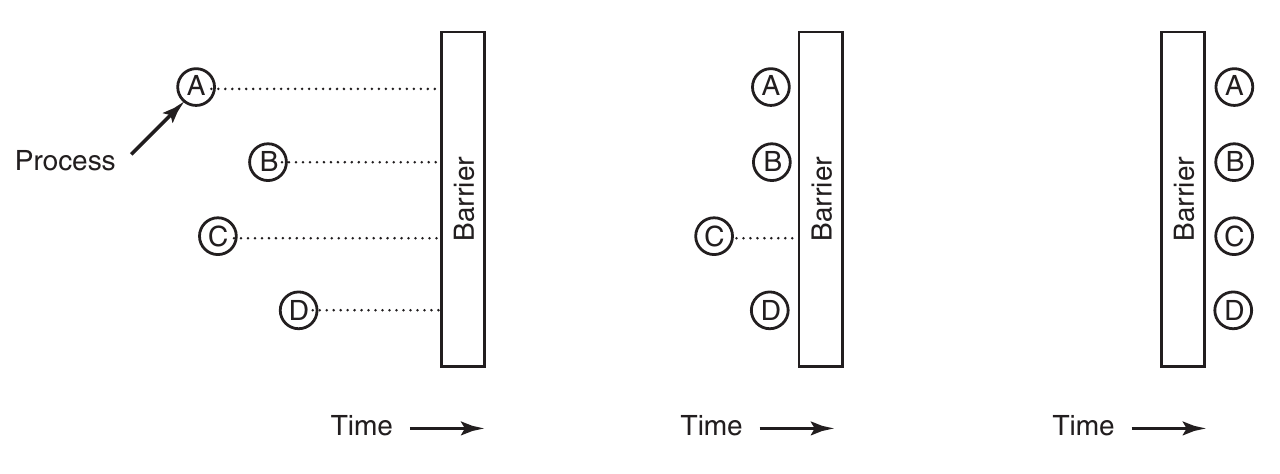
\includegraphics[width=0.9\paperwidth]{resources/barreira}
	\end{figure}
\end{frame}
\begin{frame}{Condições de corrida}
	\framesubtitle{Evitando bloquear: read-copy-update}
	\begin{itemize}
		\item Algumas situações exigem que haja limitação no acesso simultâneo a estruturas de dados
		\begin{itemize}
			\item \textbf{Exemplo:} um processo ordenando um vetor de números enquanto o outro calcula a média
		\end{itemize}
		\item Em situações específicas é possível organizar o código de forma a permitir que vários processos acessem os dados ao mesmo tempo sem necessidade de sincronização
		\item Precisamos garantir que todos os leitores vejam a versão antiga ou a nova de uma estrutura de dados, mas nunca uma combinação das duas
		\item Ao excluir um item, devemos garantir que nenhum processo possui uma referência ao dado excluído antes de liberar a memória
	\end{itemize}
\end{frame}
\begin{frame}{Condições de corrida}
	\framesubtitle{Evitando bloquear: read-copy-update}
	\begin{figure}
		\only<1>{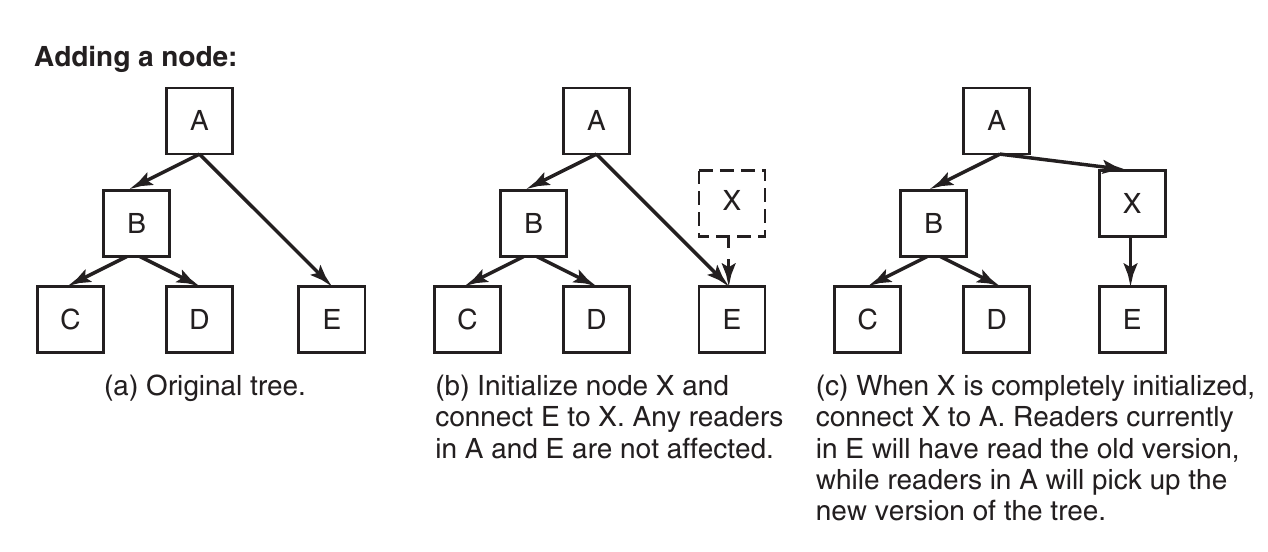
\includegraphics[width=0.9\paperwidth]{resources/rcu1}}
		\only<2>{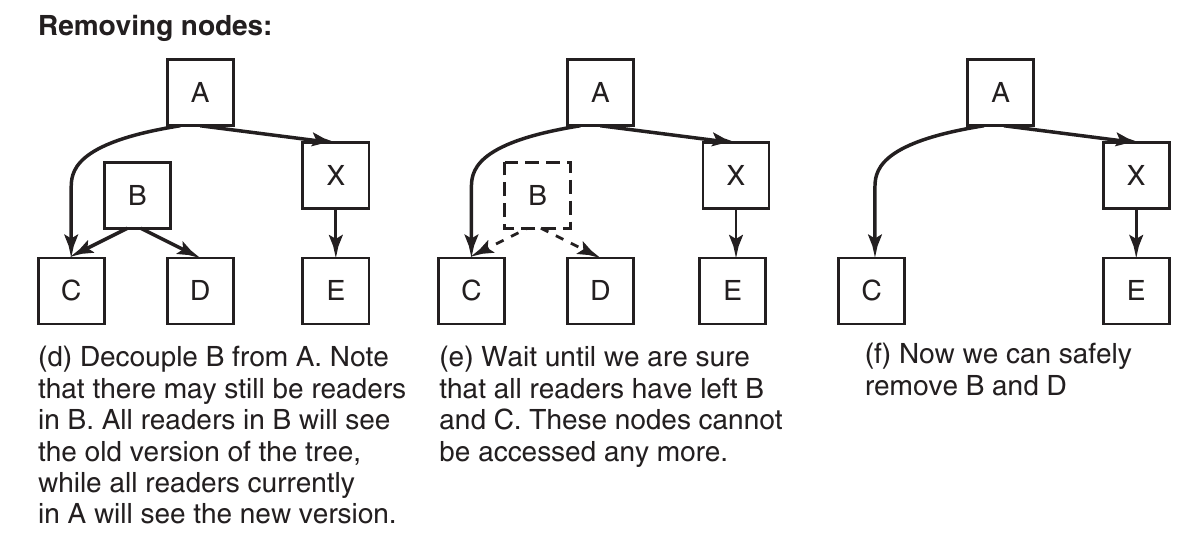
\includegraphics[width=0.9\paperwidth]{resources/rcu2}}
	\end{figure}
\end{frame}
\section{Escalonamento}
\begin{frame}{Escalonamento}
	\begin{itemize}
		\item Quando dois ou mais processos estão no estado \textbf{pronto}, eles disputam a posse da CPU
		\item É papel do \textbf{escalonador} distribuir o tempo de CPU adequadamente entre os processos que desejam utilizá-la
		\item Threads também precisam ser escalonadas
		\item Processadores com múltiplos cores serão abordados mais adiante no curso
	\end{itemize}
\end{frame}
\begin{frame}{Escalonamento}
	\begin{itemize}
		\item Situações diferentes exigem algoritmos de escalonamento diferente:
		\begin{itemize}
			\item \textbf{Sistemas em lote:} ao terminar um lote, execute o outro
			\item \textbf{Computadores pessoais:} o usuário, em geral, utiliza um programa de cada vez (nem tanto)
			\item \textbf{Servidores:} é bom dar preferência a processos que estão atendendo os usuários
			\item \textbf{Dispositivos móveis:} há limitação no poder de processamento e no uso de bateria
		\end{itemize}
		\item Além disso, a troca de processos é computacionalmente cara
	\end{itemize}
\end{frame}
\begin{frame}{Escalonamento}
	\framesubtitle{Comportamento de processos}
	\begin{itemize}
		\item Processos alternam entre utilizar a CPU e fazer I/O
		\item Podemos classificar os processos como: \textbf{limitados por I/O} ou \textbf{limitados por CPU}
	\end{itemize}
	\begin{figure}
		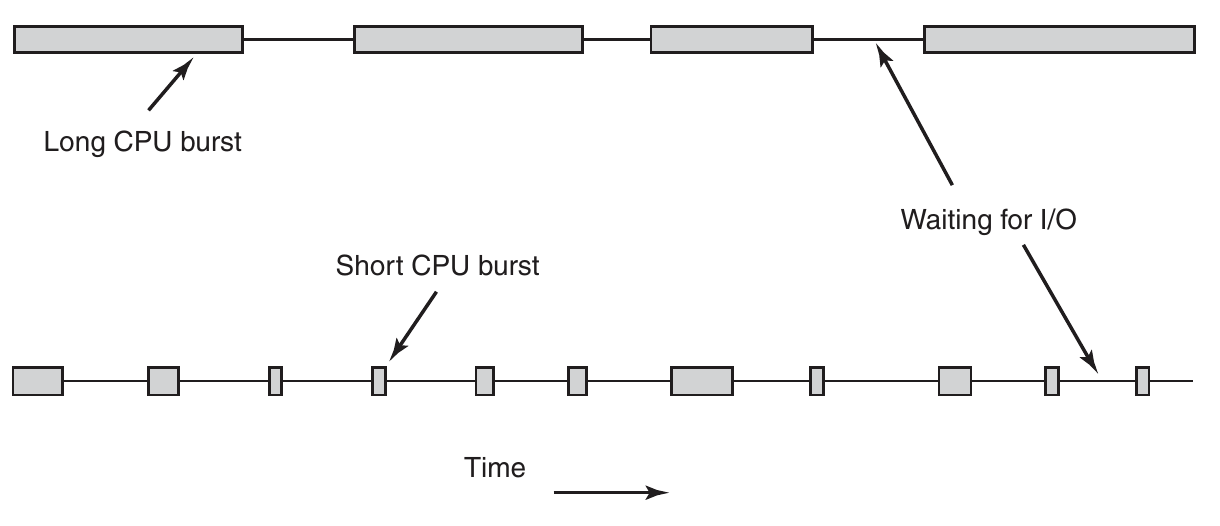
\includegraphics[width=0.8\paperwidth]{resources/iocpubound}
	\end{figure}
\end{frame}
\begin{frame}{Escalonamento}
	\framesubtitle{Quando escalonar?}
	\begin{itemize}
		\item Quando um processo é criado: executamos o processo pai ou o processo filho?
		\item Quando um processo termina
		\item Quando um processo bloqueia (esperando I/O, fazendo \texttt{down} em um semáforo, etc.)
		\item Quando ocorre uma interrupção de I/O: executamos o processo que acaba de ir para o estado pronto, o processo que estava rodando antes da interrupção ou outro processo?
		\item Quando ocorre uma interrupção de clock
	\end{itemize}
\end{frame}
\begin{frame}{Escalonamento}
	\framesubtitle{Quando escalonar?}
	\begin{itemize}
		\item Um algoritmo de escalonamento pode ser:
		\begin{itemize}
			\item \textbf{Não-preemptivo:} nunca interrompe um processo. A troca de processos só ocorre quando o processo bloqueia ou voluntariamente cede a CPU
			\item \textbf{Preemptivo:} o processo roda por um tempo prefixado e então é retirado da CPU. Requer o uso de uma interrupção de clock
		\end{itemize}
	\end{itemize}
\end{frame}
\begin{frame}{Escalonamento}
	\framesubtitle{Tipos de algoritmos de escalonamento}
	\begin{itemize}
		\item Em ambientes com execução em \textbf{lotes} (mainframes), em geral podemos utilizar algoritmos não preemptivos, pois não temos urgência em atender o usuário
		\item Num ambiente \textbf{interativo} (ex.: computador pessoal), algoritmos preemptivos são fundamentais para evitar que um processo tome controle total da CPU
		\item Em sistemas de \textbf{tempo real}, por vezes algoritmos preemptivos não são necessários, pois os processos são projetados para colaobrarem entre si
	\end{itemize}
\end{frame}
\begin{frame}{Escalonamento}
	\framesubtitle{Objetivos do algoritmo de escalonamento}
	\begin{itemize}
		\item Dependendo do ambiente, o objetivo do algoritmo de escalonamento pode mudar:
		\begin{itemize}
			\item \textbf{Todos os sistemas:}
			\begin{itemize}
				\item \textbf{Justiça:} dar a cada processo um tempo justo de CPU
				\item \textbf{Aplicação de política:} garantir que determinada política de escalonamento seja cumprida (ex.: alguns processos têm mais prioridade que outros)
				\item \textbf{Equilíbrio:} manter todas as partes do sistema ocupadas (misturar processos limitados por I/O e por CPU para manter o disco e a CPU ocupados)
			\end{itemize}
		\end{itemize}
	\end{itemize}
\end{frame}
\begin{frame}{Escalonamento}
	\framesubtitle{Objetivos do algoritmo de escalonamento}
	\begin{itemize}
		\item Dependendo do ambiente, o objetivo do algoritmo de escalonamento pode mudar:
		\begin{itemize}
			\item \textbf{Sistemas em lotes:}
			\begin{itemize}
				\item \textbf{Vazão (throughput):} maximizar número de jobs por hora
				\item \textbf{Tempo de retorno:} minimizar o tempo entre a submissão de um job e o seu término
				\item \textbf{Utilização da CPU:} manter a CPU ocupada a maior parte do tempo
			\end{itemize}
		\end{itemize}
	\end{itemize}
\end{frame}
\begin{frame}{Escalonamento}
	\framesubtitle{Objetivos do algoritmo de escalonamento}
	\begin{itemize}
		\item Dependendo do ambiente, o objetivo do algoritmo de escalonamento pode mudar:
		\begin{itemize}
			\item \textbf{Sistemas interativos:}
			\begin{itemize}
				\item \textbf{Tempo de resposta:} responder requisições rapidamente (requisições do usuário tem precedência sobre processos em plano de fundo)
				\item \textbf{Proporcionalidade:} atender às expectativas do usuário (ex.: fechar uma conexão deve ser mais rápido que fazer o upload de um arquivo grande)
			\end{itemize}
		\end{itemize}
	\end{itemize}
\end{frame}
\begin{frame}{Escalonamento}
	\framesubtitle{Objetivos do algoritmo de escalonamento}
	\begin{itemize}
		\item Dependendo do ambiente, o objetivo do algoritmo de escalonamento pode mudar:
		\begin{itemize}
			\item \textbf{Sistemas de tempo real:}
			\begin{itemize}
				\item \textbf{Cumprir prazos:} evitar perda de dados
				\item \textbf{Previsibilidade:} evitar degradação de qualidade em sistemas multimídia
			\end{itemize}
			\item Não veremos escalonamento pra sistemas de tempo real neste curso
		\end{itemize}
	\end{itemize}
\end{frame}
\begin{frame}{Escalonamento}
	\framesubtitle{Escalonamento em sistemas em lotes}
	\begin{itemize}
		\item \textbf{Primeiro a chegar, primeiro a ser servido (first-come, first-served):}
		\begin{itemize}
			\item Algoritmo não-preemptivo
			\item Processos recebem a CPU na ordem em que a requisitam
			\item Utiliza uma fila de jobs. Processos recebem a CPU na ordem em que entram na fila
			\item Quando um processo bloqueia, volta ao final da fila
			\item Justo, simples de entender e implementar
		\end{itemize}
	\end{itemize}
\end{frame}
\begin{frame}{Escalonamento}
	\framesubtitle{Escalonamento em sistemas em lotes}
	\begin{itemize}
		\item \textbf{Primeiro a chegar, primeiro a ser servido (first-come, first-served):}
		\begin{itemize}
			\item \textbf{Problema:} um processo limitado por CPU que executa por 1 segundo cada vez que obtém a CPU, vários processos limitados por I/O que precisam realizar 1000 leituras de disco para realizar seu trabalho
			\item Cada processo limitado por I/O consegue ler um bloco do disco a cada segundo, levando 1000 segundos para terminar
			\item Se pudéssemos preemptar o processo limitado por CPU a cada 10ms, poderíamos reduziresse tempo para 10 segundos
		\end{itemize}
	\end{itemize}
\end{frame}
\begin{frame}{Escalonamento}
	\framesubtitle{Escalonamento em sistemas em lotes}
	\begin{itemize}
		\item \textbf{Jobs mais curtos primeiro:}
		\begin{itemize}
			\item Assume que temos conhecimento da duração de cada job
			\item Jobs são ordenados por sua duração, sendo os mais curtos executados primeiro
			\item É um algoritmo ótimo (garante o menor tempo de resposta possível), mas somente quando todos os jobs estão disponíveis simultaneamente
		\end{itemize}
	\end{itemize}
\end{frame}
\begin{frame}{Escalonamento}
	\framesubtitle{Escalonamento em sistemas em lotes}
	\begin{itemize}
		\item \textbf{Jobs mais curtos primeiro:}
		\begin{itemize}
			\item Tempo de resposta médio (ABCD):
			\begin{equation*}
				\frac{8 + 12 + 16 + 20}{4} = 14
			\end{equation*}
			\item Tempo de resposta médio (BCDA):
			\begin{equation*}
				 \frac{4 + 8 + 12 + 20}{4} = 11
			\end{equation*}
		\end{itemize}
	\end{itemize}
	\begin{figure}
		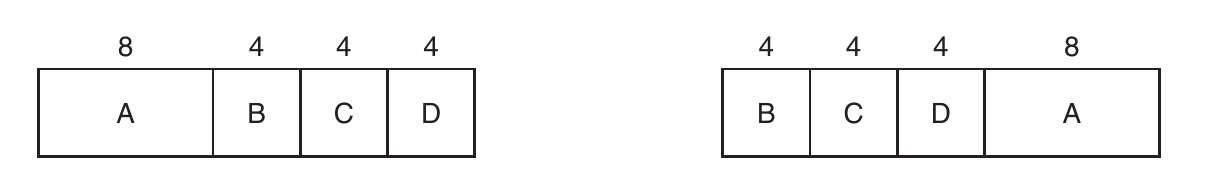
\includegraphics[width=0.8\paperwidth]{resources/shortestjob}
	\end{figure}
\end{frame}
\begin{frame}{Escalonamento}
	\framesubtitle{Escalonamento em sistemas em lotes}
	\begin{itemize}
		\item \textbf{Menor tempo restante:}
		\begin{itemize}
			\item Versão preemptiva do algoritmo anterior
			\item Quando um novo job chega ao sistema, seu tempo total é comparado com o tempo restante do job que está rodando atualmente. Se for menor, o processo atual é suspenso e o novo processo ganha a posse da CPu
			\item Requer conhecimento das durações de cada processo
			\item Oferece bom serviço a jobs de pequena duração
		\end{itemize}
	\end{itemize}
\end{frame}
\begin{frame}{Escalonamento}
	\framesubtitle{Escalonamento em sistemas interativos}
\end{frame}
\end{document}